\ifdefined\included
\else
\documentclass[a4paper,11pt,twoside]{StyleThese}
\usepackage{amsmath,amssymb, amsthm}             % AMS Math
\usepackage[T1]{fontenc}
\usepackage[utf8x]{inputenc}
\usepackage{babel}
\usepackage{datetime}

\usepackage{silence}

\WarningFilter{minitoc(hints)}{W0023}
\WarningFilter{minitoc(hints)}{W0028}
\WarningFilter{minitoc(hints)}{W0030}

\usepackage{lmodern}
\usepackage{tabularx}
%\usepackage{tabular}
\usepackage{multirow}
\usepackage{xspace}

\usepackage{subfig}
\usepackage[inline]{enumitem}

\usepackage{hhline}
\usepackage[left=1.5in,right=1.3in,top=1.1in,bottom=1.1in,includefoot,includehead,headheight=13.6pt]{geometry}
\renewcommand{\baselinestretch}{1.05}

% Table of contents for each chapter

\usepackage[nottoc, notlof, notlot]{tocbibind}
\usepackage{minitoc}
\setcounter{minitocdepth}{2}
\mtcindent=15pt
% Use \minitoc where to put a table of contents

\usepackage{aecompl}

% Glossary / list of abbreviations

\usepackage[intoc]{nomencl}
\iftoggle{ThesisInEnglish}{%
\renewcommand{\nomname}{Glossary}
}{ %
\renewcommand{\nomname}{Liste des Abréviations}
}

\usepackage{etoolbox}
\renewcommand\nomgroup[1]{%
  \item[\bfseries
  \ifstrequal{#1}{A}{Number Sets}{%
  \ifstrequal{#1}{G}{Agents Beliefs and Action Models}{%
  \ifstrequal{#1}{N}{Navigation}{%
  \ifstrequal{#1}{O}{Ontology}{%
  \ifstrequal{#1}{R}{Referring Expression Generation}{%
  \ifstrequal{#1}{Z}{Controllable and Uncontrollable Agents Task Planning}{}}}}}}%
]}

\makenomenclature



% My pdf code

\usepackage{ifpdf}

\ifpdf
  \usepackage[pdftex]{graphicx}
  \DeclareGraphicsExtensions{.jpg}
  \usepackage[pagebackref,hyperindex=true]{hyperref}
  \usepackage{tikz}
  \usetikzlibrary{arrows,shapes,calc}
\else
  \usepackage{graphicx}
  \DeclareGraphicsExtensions{.ps,.eps}
  \usepackage[dvipdfm,pagebackref,hyperindex=true]{hyperref}
\fi

\graphicspath{{.}{images/}}

%% nicer backref links. NOTE: The flag ThesisInEnglish is used to define the
% language in the back references. Read more about it in These.tex

\iftoggle{ThesisInEnglish}{%
\renewcommand*{\backref}[1]{}
\renewcommand*{\backrefalt}[4]{%
\ifcase #1 %
(Not cited.)%
\or
(Cited in page~#2.)%
\else
(Cited in pages~#2.)%
\fi}
\renewcommand*{\backrefsep}{, }
\renewcommand*{\backreftwosep}{ and~}
\renewcommand*{\backreflastsep}{ and~}
}{%
\renewcommand*{\backref}[1]{}
\renewcommand*{\backrefalt}[4]{%
\ifcase #1 %
(Non cité.)%
\or
(Cité en page~#2.)%
\else
(Cité en pages~#2.)%
\fi}
\renewcommand*{\backrefsep}{, }
\renewcommand*{\backreftwosep}{ et~}
\renewcommand*{\backreflastsep}{ et~}
}

% Links in pdf
\usepackage{color}
\definecolor{linkcol}{rgb}{0,0,0.4} 
\definecolor{citecol}{rgb}{0.5,0,0} 
\definecolor{linkcol}{rgb}{0,0,0} 
\definecolor{citecol}{rgb}{0,0,0}
% Change this to change the informations included in the pdf file

\hypersetup
{
bookmarksopen=true,
pdftitle="Endowing the robot with the abilities to control and evaluate its contribution to a human-robot joint action",
pdfauthor="Amandine MAYIMA", %auteur du document
pdfsubject="Thèse", %sujet du document
%pdftoolbar=false, %barre d'outils non visible
pdfmenubar=true, %barre de menu visible
pdfhighlight=/O, %effet d'un clic sur un lien hypertexte
colorlinks=true, %couleurs sur les liens hypertextes
pdfpagemode=None, %aucun mode de page
pdfpagelayout=SinglePage, %ouverture en simple page
pdffitwindow=true, %pages ouvertes entierement dans toute la fenetre
linkcolor=linkcol, %couleur des liens hypertextes internes
citecolor=citecol, %couleur des liens pour les citations
urlcolor=linkcol %couleur des liens pour les url
}

% definitions.
% -------------------

\setcounter{secnumdepth}{3}
\setcounter{tocdepth}{2}

% Some useful commands and shortcut for maths:  partial derivative and stuff

\newcommand{\pd}[2]{\frac{\partial #1}{\partial #2}}
\def\abs{\operatorname{abs}}
\def\argmax{\operatornamewithlimits{arg\,max}}
\def\argmin{\operatornamewithlimits{arg\,min}}
\def\diag{\operatorname{Diag}}
\newcommand{\eqRef}[1]{(\ref{#1})}

\usepackage{rotating}                    % Sideways of figures & tables
%\usepackage{bibunits}
%\usepackage[sectionbib]{chapterbib}          % Cross-reference package (Natural BiB)
%\usepackage{natbib}                  % Put References at the end of each chapter
                                         % Do not put 'sectionbib' option here.
                                         % Sectionbib option in 'natbib' will do.
\usepackage{fancyhdr}                    % Fancy Header and Footer

% \usepackage{txfonts}                     % Public Times New Roman text & math font
  
%%% Fancy Header %%%%%%%%%%%%%%%%%%%%%%%%%%%%%%%%%%%%%%%%%%%%%%%%%%%%%%%%%%%%%%%%%%
% Fancy Header Style Options

\pagestyle{fancy}                       % Sets fancy header and footer
\fancyfoot{}                            % Delete current footer settings

%\renewcommand{\chaptermark}[1]{         % Lower Case Chapter marker style
%  \markboth{\chaptername\ \thechapter.\ #1}}{}} %

%\renewcommand{\sectionmark}[1]{         % Lower case Section marker style
%  \markright{\thesection.\ #1}}         %

\fancyhead[LE,RO]{\bfseries\thepage}    % Page number (boldface) in left on even
% pages and right on odd pages
\fancyhead[RE]{\bfseries\nouppercase{\leftmark}}      % Chapter in the right on even pages
\fancyhead[LO]{\bfseries\nouppercase{\rightmark}}     % Section in the left on odd pages

\let\headruleORIG\headrule
\renewcommand{\headrule}{\color{black} \headruleORIG}
\renewcommand{\headrulewidth}{1.0pt}
\usepackage{colortbl}
\arrayrulecolor{black}

\fancypagestyle{plain}{
  \fancyhead{}
  \fancyfoot{}
  \renewcommand{\headrulewidth}{0pt}
}

%\usepackage{MyAlgorithm}
%\usepackage[noend]{MyAlgorithmic}
\usepackage{algorithm}
\usepackage[noend]{algpseudocode}
\usepackage{comment}
\usepackage[ED=MITT-InfoTel, Ets=INSA]{tlsflyleaf}
%%% Clear Header %%%%%%%%%%%%%%%%%%%%%%%%%%%%%%%%%%%%%%%%%%%%%%%%%%%%%%%%%%%%%%%%%%
% Clear Header Style on the Last Empty Odd pages
\makeatletter

\def\cleardoublepage{\clearpage\if@twoside \ifodd\c@page\else%
  \hbox{}%
  \thispagestyle{empty}%              % Empty header styles
  \newpage%
  \if@twocolumn\hbox{}\newpage\fi\fi\fi}

\newcommand*{\algrule}[1][\algorithmicindent]{%
	\makebox[#1][l]{%
		\hspace*{.2em}% <------------- This is where the rule starts from
		\vrule height .75\baselineskip depth .25\baselineskip
	}
}

%%% to have lines in algorithm, from stackexchange
\newcount\ALG@printindent@tempcnta
\def\ALG@printindent{%
	\ifnum \theALG@nested>0% is there anything to print
	\ifx\ALG@text\ALG@x@notext% is this an end group without any text?
	% do nothing
	\else
	\unskip
	% draw a rule for each indent level
	\ALG@printindent@tempcnta=1
	\loop
	\algrule[\csname ALG@ind@\the\ALG@printindent@tempcnta\endcsname]%
	\advance \ALG@printindent@tempcnta 1
	\ifnum \ALG@printindent@tempcnta<\numexpr\theALG@nested+1\relax
	\repeat
	\fi
	\fi
}
% the following line injects our new indent handling code in place of the default spacing
\patchcmd{\ALG@doentity}{\noindent\hskip\ALG@tlm}{\ALG@printindent}{}{\errmessage{failed to patch}}
\patchcmd{\ALG@doentity}{\item[]\nointerlineskip}{}{}{} % no spurious vertical space
% end vertical rule patch for algorithmicx

\makeatother
 
%%%%%%%%%%%%%%%%%%%%%%%%%%%%%%%%%%%%%%%%%%%%%%%%%%%%%%%%%%%%%%%%%%%%%%%%%%%%%%% 
% Prints your review date and 'Draft Version' (From Josullvn, CS, CMU)
\newcommand{\reviewtimetoday}[2]{\special{!userdict begin
    /bop-hook{gsave 20 710 translate 45 rotate 0.8 setgray
      /Times-Roman findfont 12 scalefont setfont 0 0   moveto (#1) show
      0 -12 moveto (#2) show grestore}def end}}
% You can turn on or off this option.
% \reviewtimetoday{\today}{Draft Version}
%%%%%%%%%%%%%%%%%%%%%%%%%%%%%%%%%%%%%%%%%%%%%%%%%%%%%%%%%%%%%%%%%%%%%%%%%%%%%%% 

\newenvironment{maxime}[1]
{
\vspace*{0cm}
\hfill
\begin{minipage}{0.5\textwidth}%
%\rule[0.5ex]{\textwidth}{0.1mm}\\%
\hrulefill $\:$ {\bf #1}\\
%\vspace*{-0.25cm}
\it 
}%
{%

\hrulefill
\vspace*{0.5cm}%
\end{minipage}
}

\let\minitocORIG\minitoc
\renewcommand{\minitoc}{\minitocORIG \vspace{1.5em}}

\usepackage{multirow}
%\usepackage{slashbox}

\newenvironment{bulletList}%
{ \begin{list}%
	{\tiny$\bullet$}%
	{\setlength{\labelwidth}{25pt}%
	 \setlength{\leftmargin}{30pt}%
	 \setlength{\itemsep}{-0.5em}}}%
{ \end{list} }

\newenvironment{inlineEnumerate}
{\begin{enumerate*} [label={(\arabic*)}] }
{\end{enumerate*}}

\theoremstyle{definition}
\newtheorem{definition}{Definition}
\renewcommand{\epsilon}{\varepsilon}

% centered page environment

\newenvironment{vcenterpage}
{\newpage\vspace*{\fill}\thispagestyle{empty}\renewcommand{\headrulewidth}{0pt}}
{\vspace*{\fill}}

\newenvironment{asl}{\ttfamily\begin{tabbing}~~~\=$\leftarrow$ \= ~~~ \=
		\kill}{\end{tabbing}}

\usepackage{tablefootnote}

\theoremstyle{plain}
\newtheorem{constraint}{Constraint}[section]

\algnewcommand\algorithmicforeach{\textbf{for each}}
\algnewcommand\algorithmicin{\textbf{in}}
\algdef{S}[FOR]{ForEach}[2]{\algorithmicforeach\ #1\ \algorithmicin\ #2\ \algorithmicdo}

\algnewcommand\algorithmicforkxor{\textbf{do fork-join-xor}}
\algnewcommand\algorithmicendforkxor{\textbf{end fork-join-xor}}
\algdef{SE}{ForkXor}{EndForkXor}{\algorithmicforkxor}{\algorithmicendforkxor}


\usepackage{listings}
\lstset{
	frame=single,
	captionpos=b,
	breaklines=true,
	basicstyle=\ttfamily,
	numberstyle=\color{black},
	tabsize=2,
	mathescape=true,
	literate=%
		{â}{{\^a}}1
}

\lstdefinestyle{inline}{
	frame=none,
	aboveskip=\smallskipamount,
	belowskip=\smallskipamount,
}

\lstdefinestyle{OwlTurtle}{
	language=C,
	tabsize=4,
	basicstyle=\scriptsize\ttfamily,
	keywordstyle=\bfseries\color{darkgray},
	morekeywords={rdf:type, rdfs:domain, rdfs:subPropertyOf, rdfs:range, :hasSubtask, :DecompositionUsedBy, rdfs:subClassOf, :hasDecomposition, owl:inverseOf, htn_actions:hasEffect, rdfs:label},
	alsoletter=:
}

\lstdefinestyle{aslDef}{
	frame=none,
%	breaklines=false,
	%xleftmargin=.1\textwidth, xrightmargin=.1\textwidth
}

\fancypagestyle{example}{%
	\fancyhead[LE]{\bfseries\thepage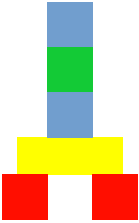
\includegraphics[scale=0.20]{figures/chapter2/task_goal.pdf}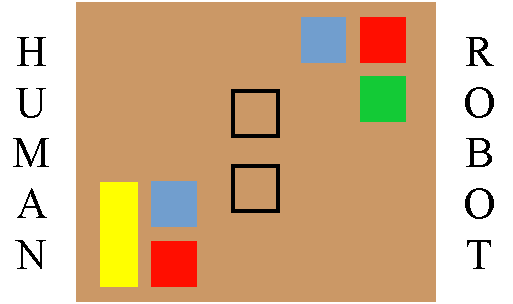
\includegraphics[scale=0.18]{figures/chapter2/task_setup_mini.pdf}}   
	\fancyhead[RO]{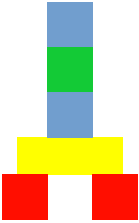
\includegraphics[scale=0.20]{figures/chapter2/task_goal.pdf}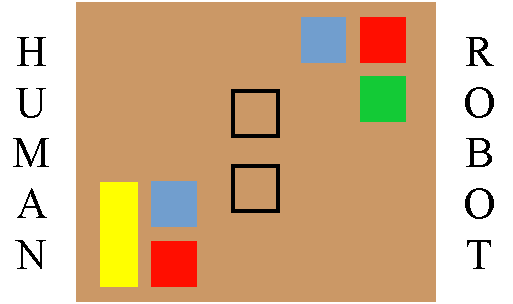
\includegraphics[scale=0.18]{figures/chapter2/task_setup_mini.pdf}\bfseries\thepage}  
	\fancyhead[RE]{\bfseries\nouppercase{\leftmark}}      % Chapter in the right on even pages
	\fancyhead[LO]{\bfseries\nouppercase{\rightmark}}     % Section in the left on odd pages
}%

\usepackage{pdfpages}
\usepackage{makecell}
\usepackage{pdflscape} 
\usepackage{mathtools}
\usepackage[section]{placeins}
\usepackage{afterpage}

%%%%%%%% my commands
\newcommand{\etal}{\textit{et al}.}
\newcommand{\ie}{\textit{i.e.}, }
\newcommand{\eg}{\textit{e.g.}, }
\newcommand{\fact}[3]{\mbox{\textit{#1}(#2, #3)}}
\newcommand{\circledtext}[1]{\raisebox{.5pt}{\textcircled{\raisebox{-.9pt} {#1}}}}
\newcommand{\sparql}{\textsc{SPARQL}}

\newcommand{\algConst}[1]{${\scriptscriptstyle #1}$}
\newcommand{\algNormTextSub}[2]{$\text{#1}_{#2}$}

\newcommand{\aslnumber}[1]{$#1$}
\newcommand{\aslstring}[1]{\textsf{#1}}
\newcommand{\aslvar}[1]{\textcolor{purple}{\textit{#1}}}
\newcommand{\asllabel}[1]{\textbf{#1}}
\newcommand{\annotation}[1]{{\footnotesize #1}}
\newcommand{\rulebody}[1]{\mbox{\hspace{.05\linewidth}}\begin{minipage}[t]{0.9\linewidth}#1.\end{minipage}}
\newcommand{\context}[1]{\begin{minipage}[t]{0.9\linewidth}#1\end{minipage}}
\newcommand{\planbody}[1]{\begin{minipage}[t]{0.9\linewidth}#1.\end{minipage}}
\newcommand{\Jason}[0]{\textbf{\textit{Jason}}}
\newcommand{\sn}{\mbox{\large\textbf{\texttt{\textasciitilde}}}}


\sloppy
\begin{document}
	\setcounter{chapter}{7} %% Numéro du chapitre précédent ;)
	\dominitoc
	\faketableofcontents
	\fi

\chapter{A direction-giving robot in a mall}
\label{chapter:chap8}
\minitoc

This chapter is based on an article submitted to the  User Modeling and User-Adapted Interaction (UMUAI) Journal. This work has been achieved in collaboration with Guillaume Sarthou, Guilhem Buisan, Phani-Teja Singamaneni, Yoan Sallami, Kathleen Belhassein, and Jules Waldhart. Moreover, a video has been presented at the HRI'20 International Conference~\cite{singamaneni_2020_guiding}, visible at \url{https://youtu.be/KfOs23wFzIQ}.

In this chapter, we first give an overview of the European H2020 Project \acrfull{mummer}\footnote{\url{http://mummer-project.eu/}}. We then present the components developed by the LAAS-RIS team. The author  contributions are related to the Supervisor component, the architecture components integration, the overall system debugging, the real-world deployment and the user study.

\section{Introduction}\label{chap8:sec:intro}

In large scale indoor environments, like museums, shopping malls, or airports, the presence of large interactive screens, maps, or signs underline the importance of providing information on itineraries. However, orienting and reading maps to find one's own way may be challenging and Rossi \etal showed that people preferred a social robot over a mobile application~\cite{rossi_2018_socially}. As for signs, the wanted written information may not be within sight. People also look for information not available on visual media such as the location of a given product. That is where the robot has a role to play, bringing a new way to help people to get their bearings in large indoor environments such as shopping malls.

Therefore, in the context of the European H2020 Project \acrshort{mummer}\footnote{\url{http://mummer-project.eu/}}, we developed and deployed a social service robot in one of the largest malls of Finland, Ideapark in the city of Lemp\"a\"al\"a. This social robot is able to engage, chat with people, and guide them. We will not talk about the two first mentioned behaviors, developed by our project partners, but focus in this chapter on the direction-giving task.

As the mall has approximately 1.2 kilometers of shopping and pedestrian streets and more than 150 shops, people get easily lost. In such a large environment, having a robot guiding customers to their wanted destination would be time-consuming for the robot and would prevent this resource to be available for as many customers as possible. Inspired by the manner in which the mall employees perform this activity, we chose the solution to have a robot not accompanying people to their desired destination but rather verbally describing the route while grounding it with pointing gestures. If necessary, it moves a few meters inside its dedicated area (Figure~\ref{fig:chap3_pepper_mall}) to improve the perspective sharing with the human when pointing at a landmark, and therefore to improve the human understanding of the route. These features are unique to a robot and cannot be found on a map or an interactive screen. To endow the robot with such abilities, we built a complete implementation of a robotic architecture that has been deployed in a real-world environment, the Finnish mall. There, it ran for three months, three days a week. Here is a sum-up of the project steps:
\begin{enumerate}
	\item March 2018: beginning of the design and implementation of the direction-giving task
	\item September 2018: First tests of the task on the field, \ie in a Finnish mall
	\item June 2019 and September 2019: New tests of the direction-giving task on the field
	\item From September to December 2019 (project formal end): The robot autonomously ran three days a week in the mall (with only remote monitoring of the robot performance by our team for debugging and tuning)
	\begin{enumerate}
		\item November 2019: Integration in the \emph{Supervisor} of a preliminary version of Quality of Interaction Evaluator implementing the model described in Chapter~\ref{chapter:chap7} \\ $\Longrightarrow$ version 1 of the QoI Evaluator
		\item From November 2019 to December 2019: Around 350 direction-giving tasks were performed with usual mall customers. Bug corrections and tuning of the direction-giving task. This allowed us to improve the QoI Evaluator thanks to: \begin{inlineEnumerate}
%			[label=(\roman*)] 
			\item data collection of task failures and standard durations of the subtasks executions \item lessons drawn about metric definitions and choices. \end{inlineEnumerate} \\ $\Longrightarrow$ version 2 of the QoI Evaluator\label{list:mall}
	\end{enumerate}
	\item January 2020: User study with 35 participants to compare three direction-giving task robot behaviors, allowing to log interactions at the same time we could monitor them\footnote{The QoI Evaluator was running in background, it was not the purpose of the study.}. End of the project.\label{list:tests}
	\item March 2020: Refinement of the QoI Evaluator, \ie improvement of the metric functions and tuning of their parameters. In the lab, with the same direction-giving task than the one used in the mall, comparison of the QoI computed by the robot when it is dealing with an ``ideal'' human, a ``confused'' human and a ``non-compliant'' human. \\ $\Longrightarrow$ version 3 of the QoI Evaluator\label{list:refin}
\end{enumerate}

All along the process, we elaborated and built the system based on the joint action principles (see Chapter~\ref{chapter:chap1}). We also conducted preliminary studies and used the joint action perspective to analyze how human guides would achieve such an activity at the place where the robot was intended to be deployed. This was possible essentially because we were able to combine the results of the JointAction4HRI\footnote{\url{https://jointaction4hri.laas.fr/}} project with the \acrshort{mummer} project.

Our claim is that such an approach is relevant in the way the joint action principles provide pertinent guidelines and it is possible to effectively elaborate models and implement systems based on them. 
The output is a complete robot architecture that integrates a number of components implementing the main decisions and behaviors which have been identified. Each of them makes use of various models and decisional algorithms, all integrating explicitly human models and joint action principles and mechanisms.


The chapter is constructed as follows. In Section~\ref{sec:related-work} we provide background information about robot guides and direction-giving task and discuss about how the human partner has been considered. In Section~\ref{sec:rationale} we discuss how we model the direction-giving task as a human-robot joint action. We analyse the task based on human-human exploratory studies and decompose it into a succession of precise subtasks in Section\ref{sec:modeling}. An overview of the resulting architecture and a description of its components are presented in Section~\ref{sec:globalarchi}. Then, we present in Section~\ref{subsec:archi-integration}, the integration of the overall architecture into a physical robot and the steps until its final deployment ``into the wild''. In Section~\ref{chap8:sec:us}, we present the user study we carried out with 35 participants and its results. Finally, in Section~\ref{sec:qoi_integration}, we show how we used this task to implement the QoI Evaluator presented in Chapter~\ref{chapter:chap7}. 


\section{Related work}
\label{sec:related-work}

A number of contributions have proposed robot guides, from the first museum guides \cite{burgard_1999_museum, thrun_99, siegwart_2003_robox, clodic_2006_rackham} to more recent robot guides in large areas \cite{bauer_2009_autonomous, triebel_2016_spencer}. For example, Chen \etal{} presented a guiding robot in a shopping mall where it accompanied the customer to the desired location and pointed at the shop~\cite{chen_2017_robots}. Another example is a shopping robot helping people to find products among the aisles of a store \cite{gross_2009_toomas}. 
However, the focus in these contributions is mainly the fact that the robot is challenged to navigate until the goal destination with the presence of humans. In this context, efficient mapping and localisation in large areas, social navigation are the main concerns. This is different from our needs where the robot is voluntarily constrained for its motion to a limited area with a focus on conveying to the human the pertinent information to reach by herself the desired place.

Direction-giving tasks have been investigated in the human-robot interaction community. Kopp \etal{} describes an embodied conversational agent giving route directions using deictic gestures~\cite{kopp_2007}. A number of key contributions have been developed over the years by ATR-IRC within the Robovie robot and project. First, Okuno \etal{} developed a model for a robot providing route directions, integrating utterances, gestures, and timing~\cite{okuno_2009_providing}. The experiments explored the influence of gestures and highlighted the importance of timing in the directions-giving task. Then, Kanda and colleagues implemented a guiding behavior as part of a wider system with the robot pointing toward the first direction to take and saying ``please go that way'' and then, continuing its explanation by saying ``After that, you will see the shop on your right.''~\cite{kanda_2009_affective, kanda_2010_communication}. Their robot also gave recommendations for restaurants and shops based on customer tastes. In their following work, they presented a route perspective model attempting to represent humans' concept of route and visibility of landmarks, which they believed to match people's perception of the environment~\cite{morales_2011}. Then, Matsumoto \etal{} developed a robot able to follow a user while inferring their memory recall of shops in the visited route~\cite{matsumoto_2012_you}. When the user asked the location of other shops, it gave the route description with references to the known locations inferred with the model of the user's memory recall. Finally, Satake \etal{} showed a complete architecture of an information-providing robot able to move around a square in a mall composed of: a map, an ontology, a speech recognition system (operated), a dialog manager, a localization module, and a people tracker. As in their previous work, the robot verbalized utterances and used deictic gestures to give route directions~\cite{satake_2015_should}. 

Let us also mention the work of Bohus \etal{}, a robot providing verbal directions to people using deictic gestures coupled with spoken references~\cite{bohus_directions_2014}. For example, the robot said ``Go to the end of this hallway'', executing a pointing gesture at the same time, and then continued the explanation with sentences such as ``Turn right and keep walking down the hallway''. Iocchi \etal{} mentioned both guiding and direction providing as use cases of their system~\cite{iocchi_2015_personalized}.

Numerous other contributions can be found but,  only a few of them propose full architectures for an autonomous direction-providing robot, the most complete one being the Robovie robot presented above. One of version of the Robovie architecture is shown in Figure

\begin{figure}[!t]
	\centering
	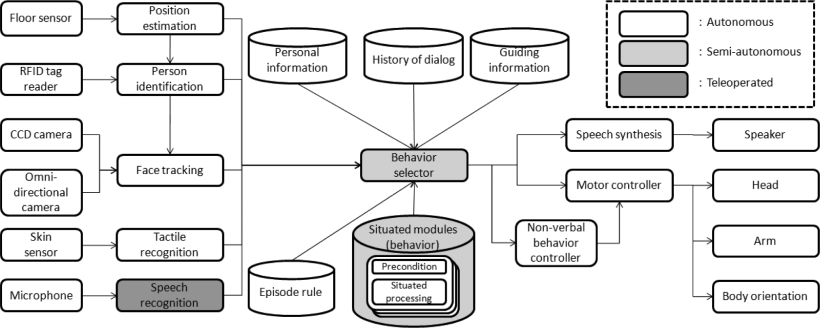
\includegraphics[width=\textwidth]{figures/chapter3/robovie_archi.png}
	\caption{\label{fig:chap3_robovie} Robovie system overview presented in~\cite{kanda_2010_communication}.}
\end{figure}

Still, to the best of our knowledge, no system tackles the overall guiding-task with flexibility. Indeed we claim that it is important for the robot to reason about the current and desired perspectives of the human and the robot and to be able to pro-actively propose to the human a pertinent placement. This is one of the basic bricks of our system and it is strongly linked to the key principles of Joint Action which involve the ability to establish and monitor joint attention,  and to conduct a multi-step task achievement involving contributions of both agents. Besides, it is the duty of the robot to permanently adapt to human needs and preferences and to synthesize acceptable behaviours.

\section{Rationale}\label{sec:rationale}

In Section~\ref{chap1:sec:ja}, we presented the concepts around joint action. In this section, we bring some new inputs specific to the direction-giving task. 

The design of our system has taken into account the results of several user studies involving human guides of the mall (see Section~\ref{sec:modeling}). Indeed, it could be of interest to have a robot performing in the same way as a human guide does as the robot would be predictable then. Indeed, ``if robots could display predictable behaviours that are in line with human's expectations based on their models of human joint action, the resulting interaction would achieve greater naturalness''~\cite[p.~17]{curioni_2017_joint} and ``human agents would then be able to apply predictive and adaptive processes acquired in human interactions to the interaction with robots''~\cite[p.17]{curioni_2017_joint}. In the context of the direction-giving task with a Pepper robot, we take advantage of the fact that the robot is a humanoid and the human anthropomorphizes the robot behaviour (whatever we do).
However, it is not always possible or desirable for a robot to imitate what a human would do at its place. It could let people think that the robot has more capabilities than it really has. In that way, besides the imitation, it could be desirable for the robot to exhibit its limitations, \eg saying that it is able to provide you direction into the mall (and nothing else).
%
%Participating agents in a joint action need to represent not only what they will do but also what will be performed by the others. Doing so, they also need to be able to consider the combined effects of their respective actions~\cite{pacherie_2012_agency}. Joint action involves representations of the other agents who are actually and potentially involved. Shared task representations provide control structures that allow agents to flexibly engage in joint action~\cite{knoblich_2011_joint}.
%

In our task, the robot has a role, it is a guide and the human is a customer with a need to find a direction. The joint action is not symmetric, there is a difference of knowledge and skills between the two agents. Curioni \etal{} raises the point that ``task asymmetry is an important factor to consider when investigating complex joint action settings because it drives the systemic emergence of communication and coordination dynamics (for example in the form of task distribution)''~\cite[p.~11]{curioni_2017_joint}. At the supervision level (see Section~\ref{subsec:supervision}), we modeled which part of the task falls to the robot and which part of the task falls to the human. We can also infer that knowing the robot role as guide, the human would be able to infer what it is entitled to do. This way, we consider that they share the route description task representation. 
Another important point is that ``shared task representations not only specify in advance the individual parts each agent is going to perform but they also govern monitoring and prediction processes that enable interpersonal coordination in real time.''~\cite[p.~65]{knoblich_2011_joint}. Our system handles that monitoring and prediction in its supervision component(see Section~\ref{subsec:supervision}).
%
%
%Joint attention provides a mechanism to form shared perceptual representations of the situation. ``The phenomenon of joint attention involves more than just two people attending to the same object or event. At least two additional conditions must be obtained. First, there must be some causal connection between the two subjects’ acts of attending (causal coordination). Second, each subject must be aware, in some sense, of the object as an object that is present to both; in other words, the fact that both are attending to the same object or event should be open or mutually manifest (mutual manifestness)''~\cite[p.~355]{pacherie_2012_agency}.
%
%As explained above, joint attention comes with two requirements: causal coordination and mutual manifestness. We can consider that the engagement in the interaction session represents the causal coordination. Then, at least on the robot side, we could argue for mutual manifestness. Indeed, as we will explain, we give the robot perspective-taking abilities, and abilities to find out where and how the human and itself should be placed to share a joint attention relative to a landmark. With those requirements fulfilled, ``by attending jointly, co-actors establish perceptual common-ground and become aware of each other's action opportunities and constraints''~\cite{curioni_2017_joint} (they also use the expression ``spatio-temporal common ground''). Joint attention and in fact in our case, the overall interaction process by itself (aka its unfolding), could be seen as an continuous process sustaining under-construction common-ground.
%

Finally, in our system, the situation assessment component provides visual perspective-taking. It computes, from the robot point of view, a number of facts regarding what the robot is looking at, which landmark is visible to it, what is present at its proximity, etc. It also computes the same information from the perspective of the person interacting with it. This way the robot is able to infer, based on its own models, which information is shared (or not) with the person it interacts with.


\section{Designing direction-giving behavior in a shopping mall}
\label{sec:modeling}

\begin{figure}[!t]
	\centering
	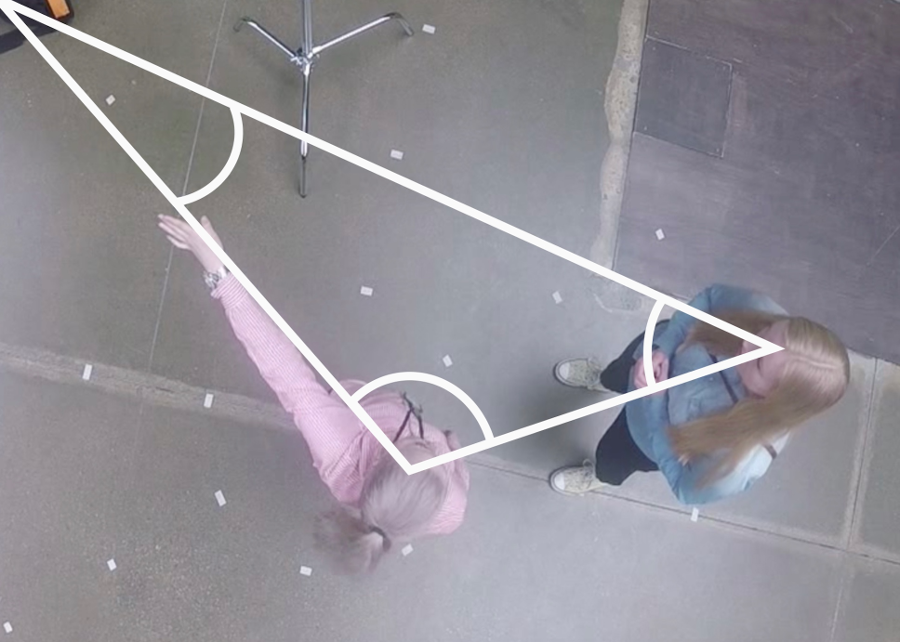
\includegraphics[scale=0.5]{figures/chapter3/human_guide.png}
	\caption{\label{fig:chap3_human_guide} Picture from the second Human-Human study~\cite{belhassein_2017_human}. Here, the guide is giving the route description to reach a given shop by pointing at it. Positions regarding the target and the customer, as well as gazes and pointing gestures, were analyzed.}
\end{figure}

\subsection{What we learnt from humans}\label{sec:methodology}
In order to inform the design and implementation of the pertinent functions and their articulation, two human-human exploratory studies were conducted in collaboration with VTT Technical Research Centre of Finland. It allowed us, in addition to the study of the existing literature, to enrich our knowledge on effective route descriptions and how they can be used in the very context of the actual robot deployment environment. 

The first pilot study consisted in a human guide providing route information. It was carried out close to the future location of the robot in order to avoid biases linked to the location or the environment. Based on preliminary interviews with guides working at Ideapark, a list of 15 shops often requested by customers was selected. The preliminary experiment consisted of one participant asking for shop directions to a guide working at the mall information booth. Two researchers, as participants, and two guides took part in the experiment. The two guides were instructed to give guidance as they would normally do. The situations were video recorded and the guides were briefly interviewed after the sessions. The video analysis focused on non-verbal communication, and in particular the different types of gestures used to give guidance, the positions of the two protagonists in relation to the target shop and their interlocutor, and the gazes alternation. Belhassein \etal{} gave the first indications to consider for the robot guidance to be effective and understood by customers, resulting from this pilot study~\cite{belhassein_2017_human}. For example, this pilot study allowed us to notice a preferential use of the ipsilateral hand to the visual field of the target. In line with the existing literature on gestures studies, we also noticed that deictic gestures were naturally more frequent than iconic gestures or beats, while metaphorical gestures were rare. As shown by Allen, the hand used to point a referent was oriented vertically in the case of stores (vertical referents) or directed actions such as a path to take or turns, whereas in the case of horizontal referents (\eg escalators), the hand was oriented horizontally (palm facing the ground)~\cite{allen_2003}.

A second exploratory study was then carried out adding complex situations (\eg two customers requesting directions at the same time, two different shops in the same request, or someone who interrupts the conversation between the guide and the customer). Again, social signals were analyzed (see Figure~\ref{fig:chap3_human_guide} for an example). The protocol used and the results have been published~\cite{heikkilae_2018_where,heikkilae_2019_should}. By analyzing the sequencing of the whole interaction, this second study showed the guide pointing the general location of the target first, before explaining and pointing the different stages of the path to take to get there. Then, the sequencing of the route description itself showed that a first deictic gesture on a visible passage (corridor, or if the shop requested is on the second floor, the escalator) preceded the explanations about the directions to take. The most interesting results concerned situations of confusion and misunderstandings. Indeed, several elements might be sources of confusion for the customer, such as using only one transmission channel (\eg gesture without speech), the choice of landmarks which are not always appropriate, if there are several route descriptions in the same explanation, or when the distance is not specified. 

\subsection{Designing of the collaborative task for a direction-giving robot}\label{sec:guiding}

From the analysis of human-human direction-giving and through an iterative design process, we designed and implemented our direction-giving robot. Our model of the collaborative task can be represented as a succession of subtasks, as shown in Figure~\ref{fig:chap3_HTN}. This figure also exhibits the incremental refinement of the task into a sequence of human-robot interactive actions. The aforementioned subtasks are:

\begin{figure}[!t]
	\centering
	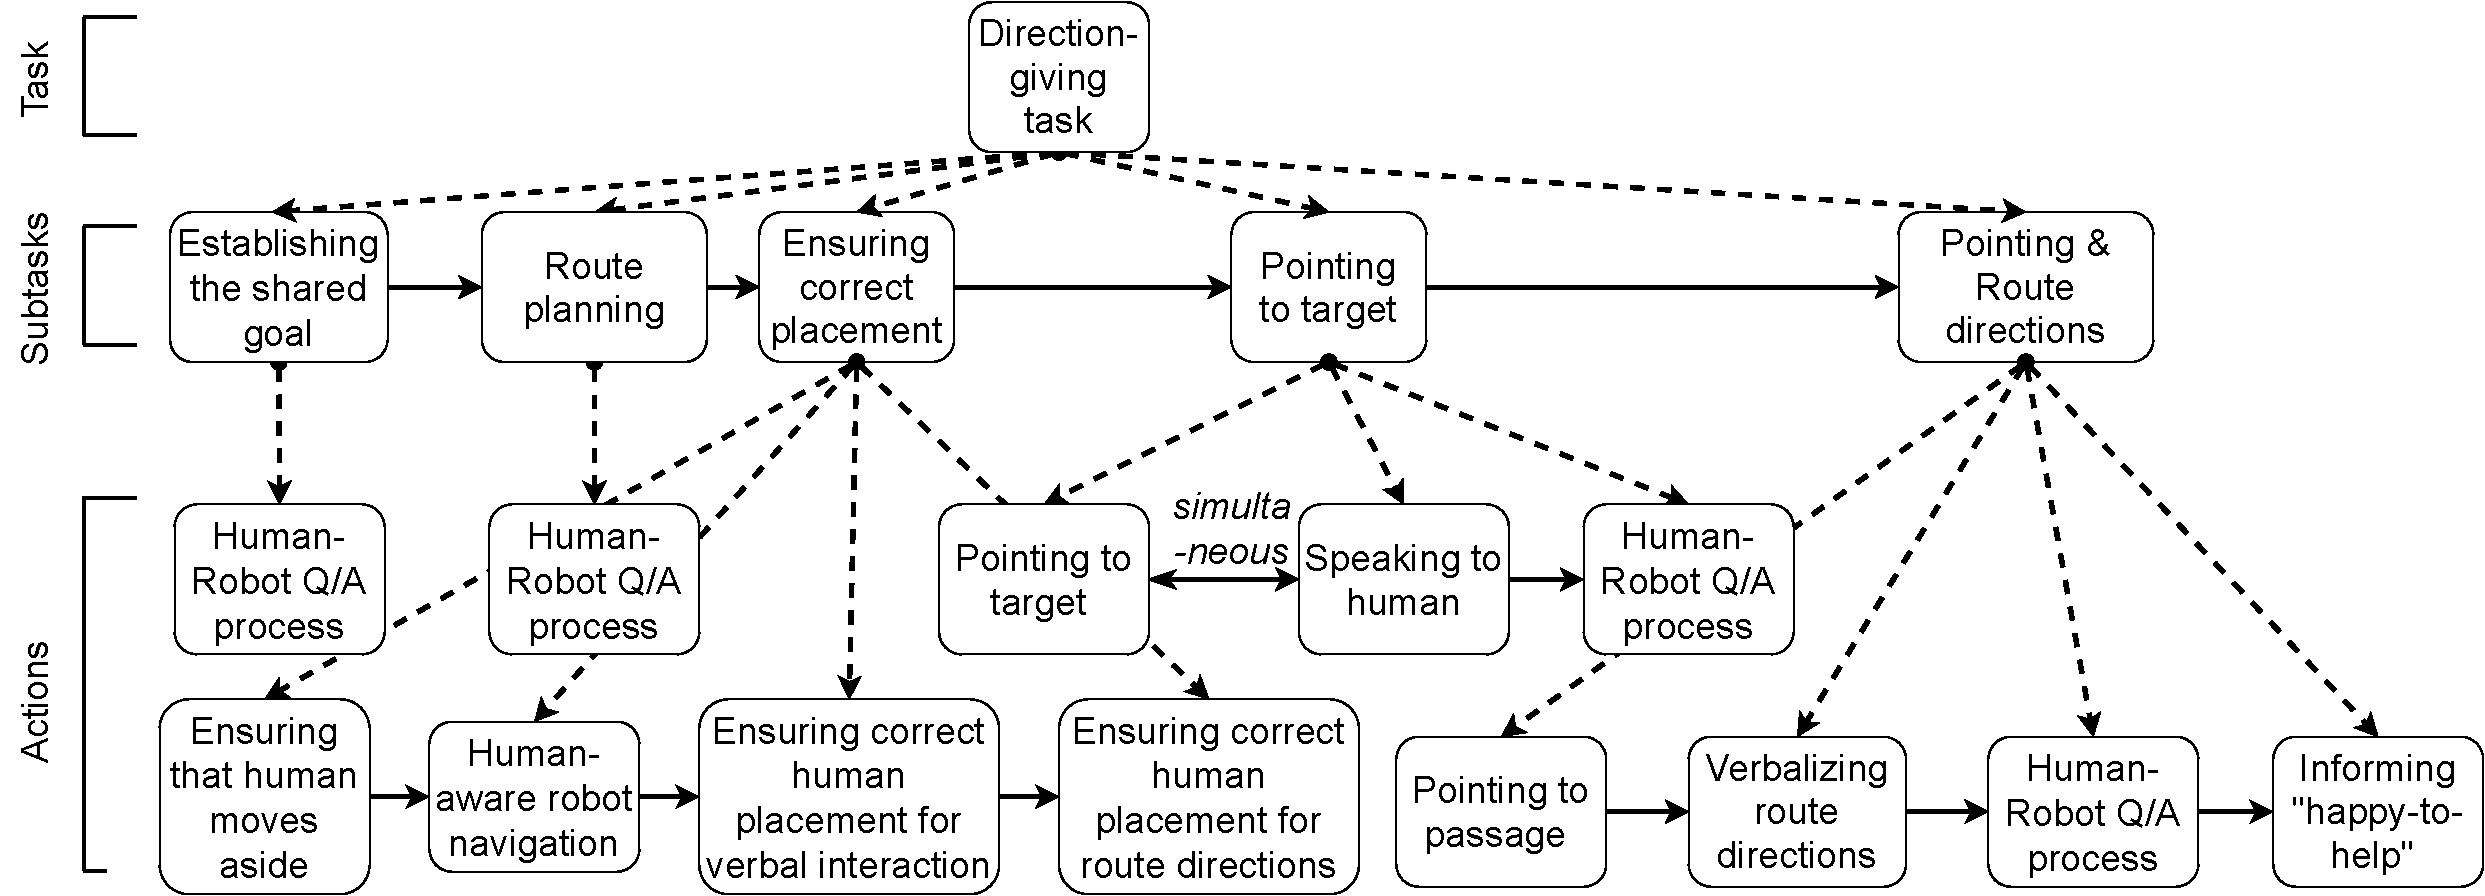
\includegraphics[width=\linewidth]{figures/chapter3/HTN-guiding_task.pdf}
	\caption{The representation of the direction-giving task as a hierarchical task network with task, substasks and actions levels. All the horizontal arrows are sequential links and the rest are decomposition ones.}
	\label{fig:chap3_HTN}
\end{figure}


\begin{enumerate}
	\item \textbf{Establishing the shared goal}: In this first step, the human and the robot negotiate and establish a shared goal. Specifically, the robot tries to determine precisely the place -- we called it the \emph{target} -- it should give directions for. This is immediately completed if the human directly asked for a known shop. Several verbal exchanges can be necessary in case the person asked for a kind of shop (\eg restaurant) or a product or in case the robot has not properly understood the name of the place and needs to disambiguate.
	\item \textbf{Route planning according to the human willingness and ability to climb stairs}: As the robot role is to help people, adapting to them, it needs to ensure that they have the abilities to follow the route it will indicate to them. So, first the robot computes the best route to the target and then checks the presence of stairs in it. In case there are, the robot enquires whether the human can or want to climb them or not. If they cannot or do not want to, the robot computes a new route without any stairs. The planned route contains a first  \emph{passage} (\ie a corridor, a door or an escalator) which the robot will try to point.
	\item \textbf{Ensuring correct placement}: The second human-human study, mentioned in Section~\ref{sec:methodology}, highlighted the fact that human guides point to a visible \emph{passage} before giving the route directions. Thus, we endowed the robot with this ability as described further in the item~\ref{steps:passage} of this list. In order to be in good conditions while performing this item \ref{steps:passage}, that is to say to ease the human understanding of the directions, the robot seeks better positions for the human and itself. It does so by computing a position for the human, considering their visual perspective of the passage.
	%Clearly, it does not planned a new position if, from it, the human visibility of the passage is not higher than their current one.
	The robot computes a new position for itself as well, to form a triangle whose vertices are the planned robot position, the planned human position and the passage, as shown in Figure~\ref{fig:chap3_human_guide} and Figure~\ref{fig:chap3_dir_giving_task}. After having computed these positions, the robot moves, and as they both are engaged in the task, expects the human to join it once its position is reached; it calls them if they do not. As the human might not be at the exact position computed for them, the robot checks their visibility of the passage. In case their visibility is too low, the robot will adjust their position thanks to verbal instructions (\ie come closer, move back). Figure~\ref{fig:chap3_dir_giving_task} illustrates the initial and final positions of both agents, in a lab context. 
	\item \textbf{Pointing to target}: Following the sequencing obtained from the aforementioned human-human study, the robot first points in the target direction, along with a brief sentence. As the robot is a helper and it is involved in a joint action with the human, it needs to ensure that its actions produce their expected results. In this case, if the robot computed that the target should be visible from their position, it checks that the human has seen it, either by monitoring their perspective or by asking. In case of a negative answer, it will point again.\label{steps:ensuring}
	\item \textbf{Pointing to passage and giving route directions}: Still following the sequencing from the study, when the target is not in the same physical space as them, meaning that there is a passage on the way to the target, the robot points to this passage and then verbalizes the route directions. These directions take into account the orientation the human will have and describe the route (\eg take the corridor on the left side). Finally, the way they are built (\ie the order of the steps, the keywords to use...) is also based on the human-human study. Here again, the robot ensures that the route directions have been understood by asking the person about it or if the passage has been seen if there is one.
	% 	(only one of the two questions is asked as with both one after the other, people interacting with the robot were annoyed). 
	In case of a negative answer, it will point and give the route directions again. Finally, the robot ends the task with a ``happy-to-help'' short sentence.\label{steps:passage}
\end{enumerate}


\begin{figure}[!ht]
	\centering
	\subfloat[Initial positions of the human and the robot. The human asked the robot for route directions to a target behind him.]{ 
		\begin{minipage}{\linewidth}\hspace{0.05\linewidth}
			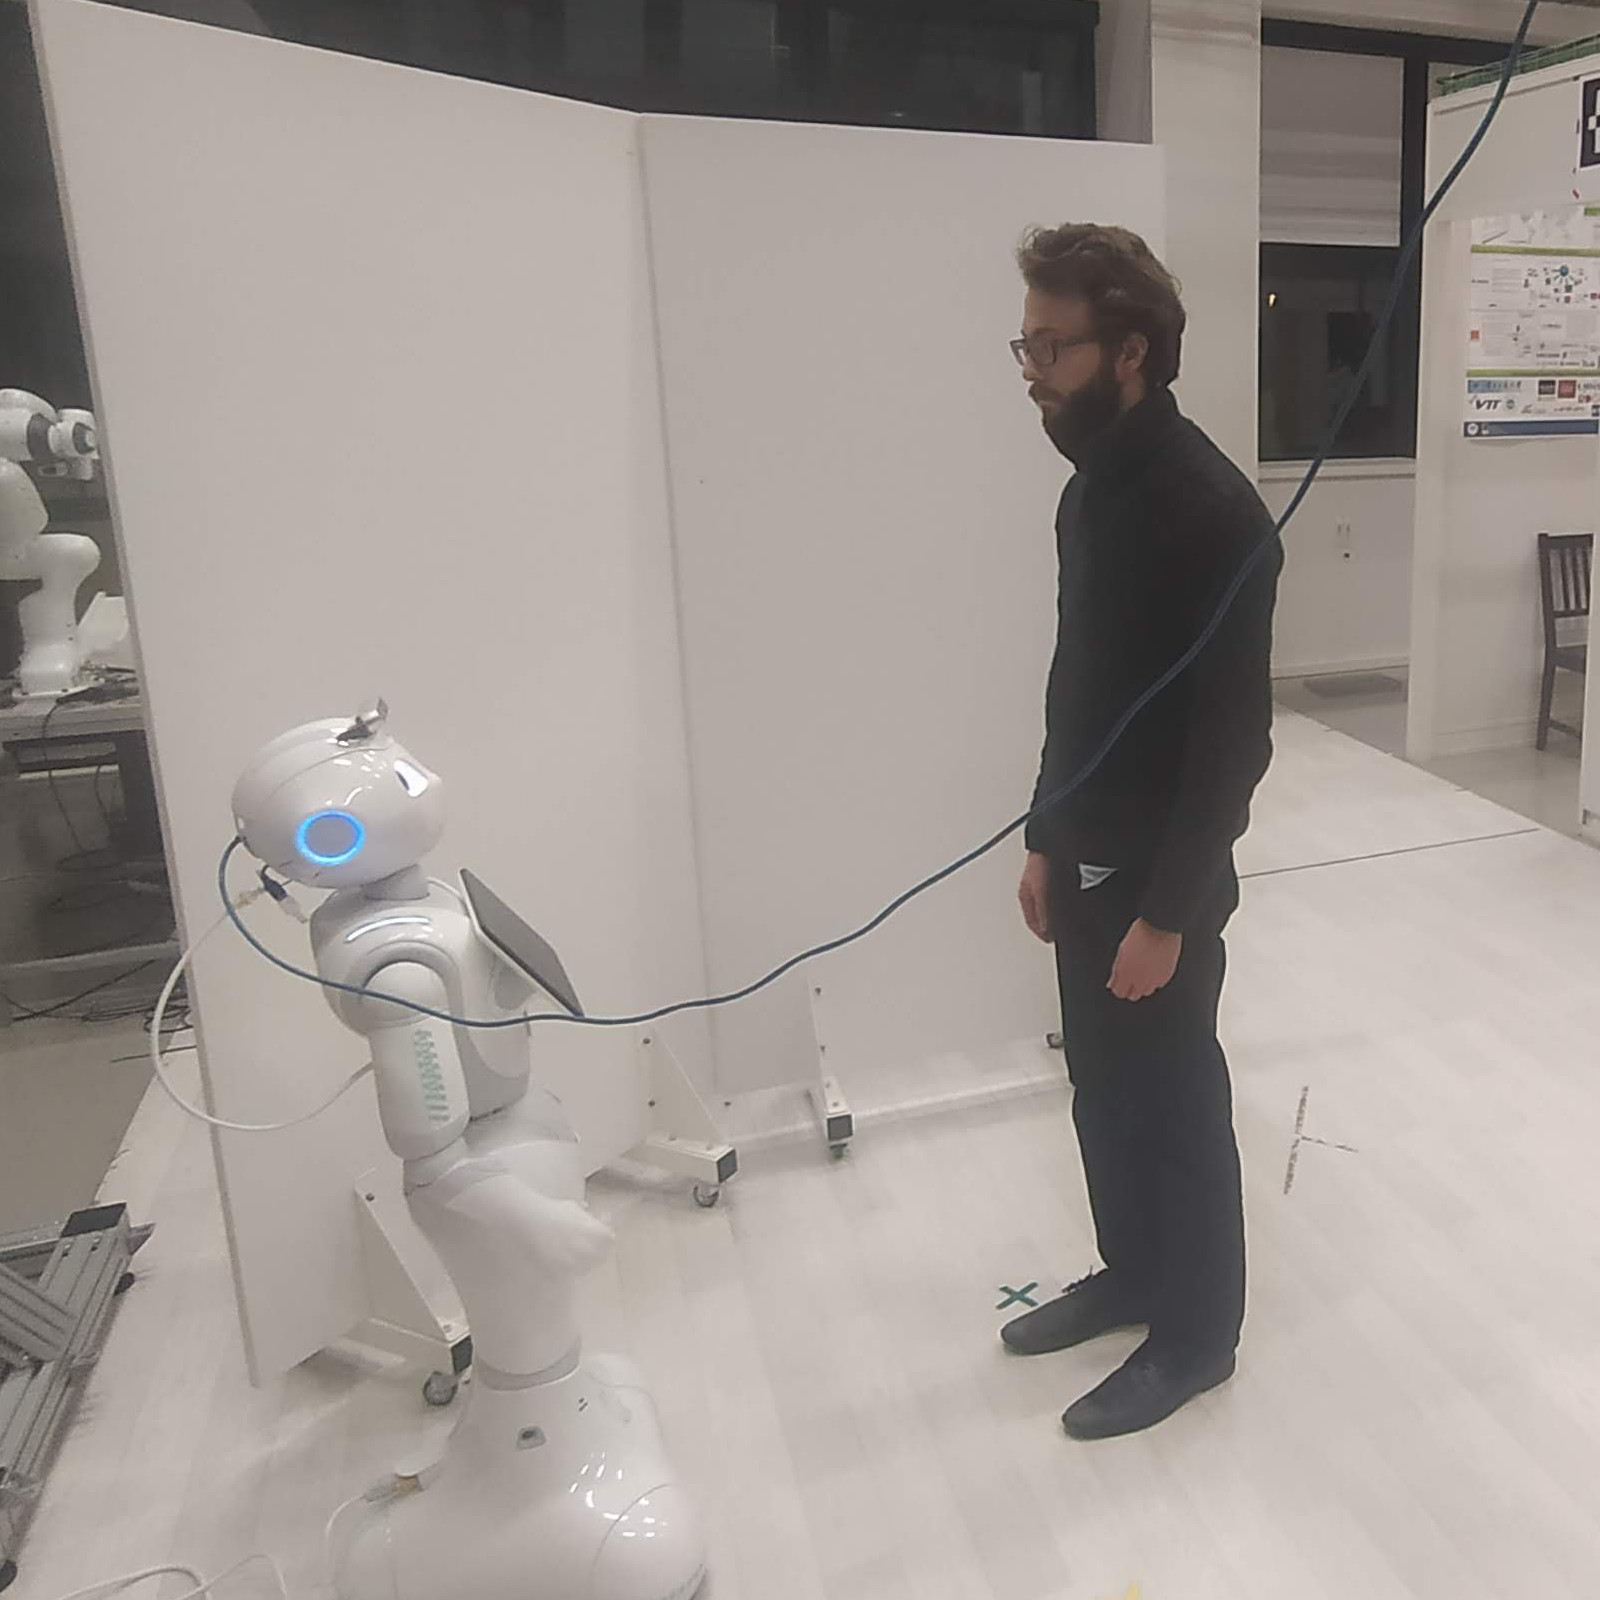
\includegraphics[width=.4\linewidth]{figures/chapter3/init_pose_r.jpg}\hspace{0.1\linewidth}
			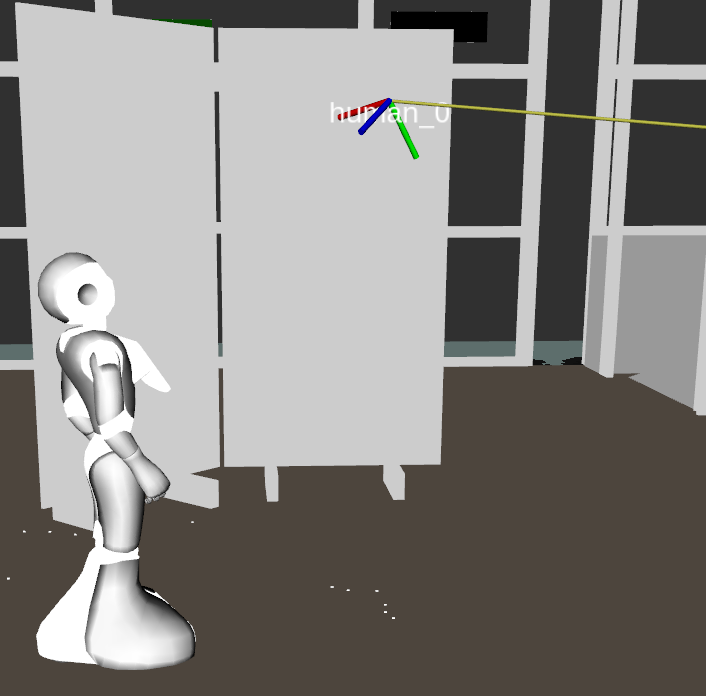
\includegraphics[width=.4\linewidth]{figures/chapter3/init_pose.png}
		\end{minipage}
	}\par\vspace{2ex}
	\subfloat[The robot and the human are in their final positions. The blue spheres are the computed position for the human by the robot. The robot is pointing to the passage (in blue frame). We can observe the triangle formed between the human, the robot and the passage (the blue area on the floor) as in Figure~\ref{fig:chap3_human_guide} where two humans are in a triangle formation.]{
		\begin{minipage}{\linewidth}\hspace{0.05\linewidth}
			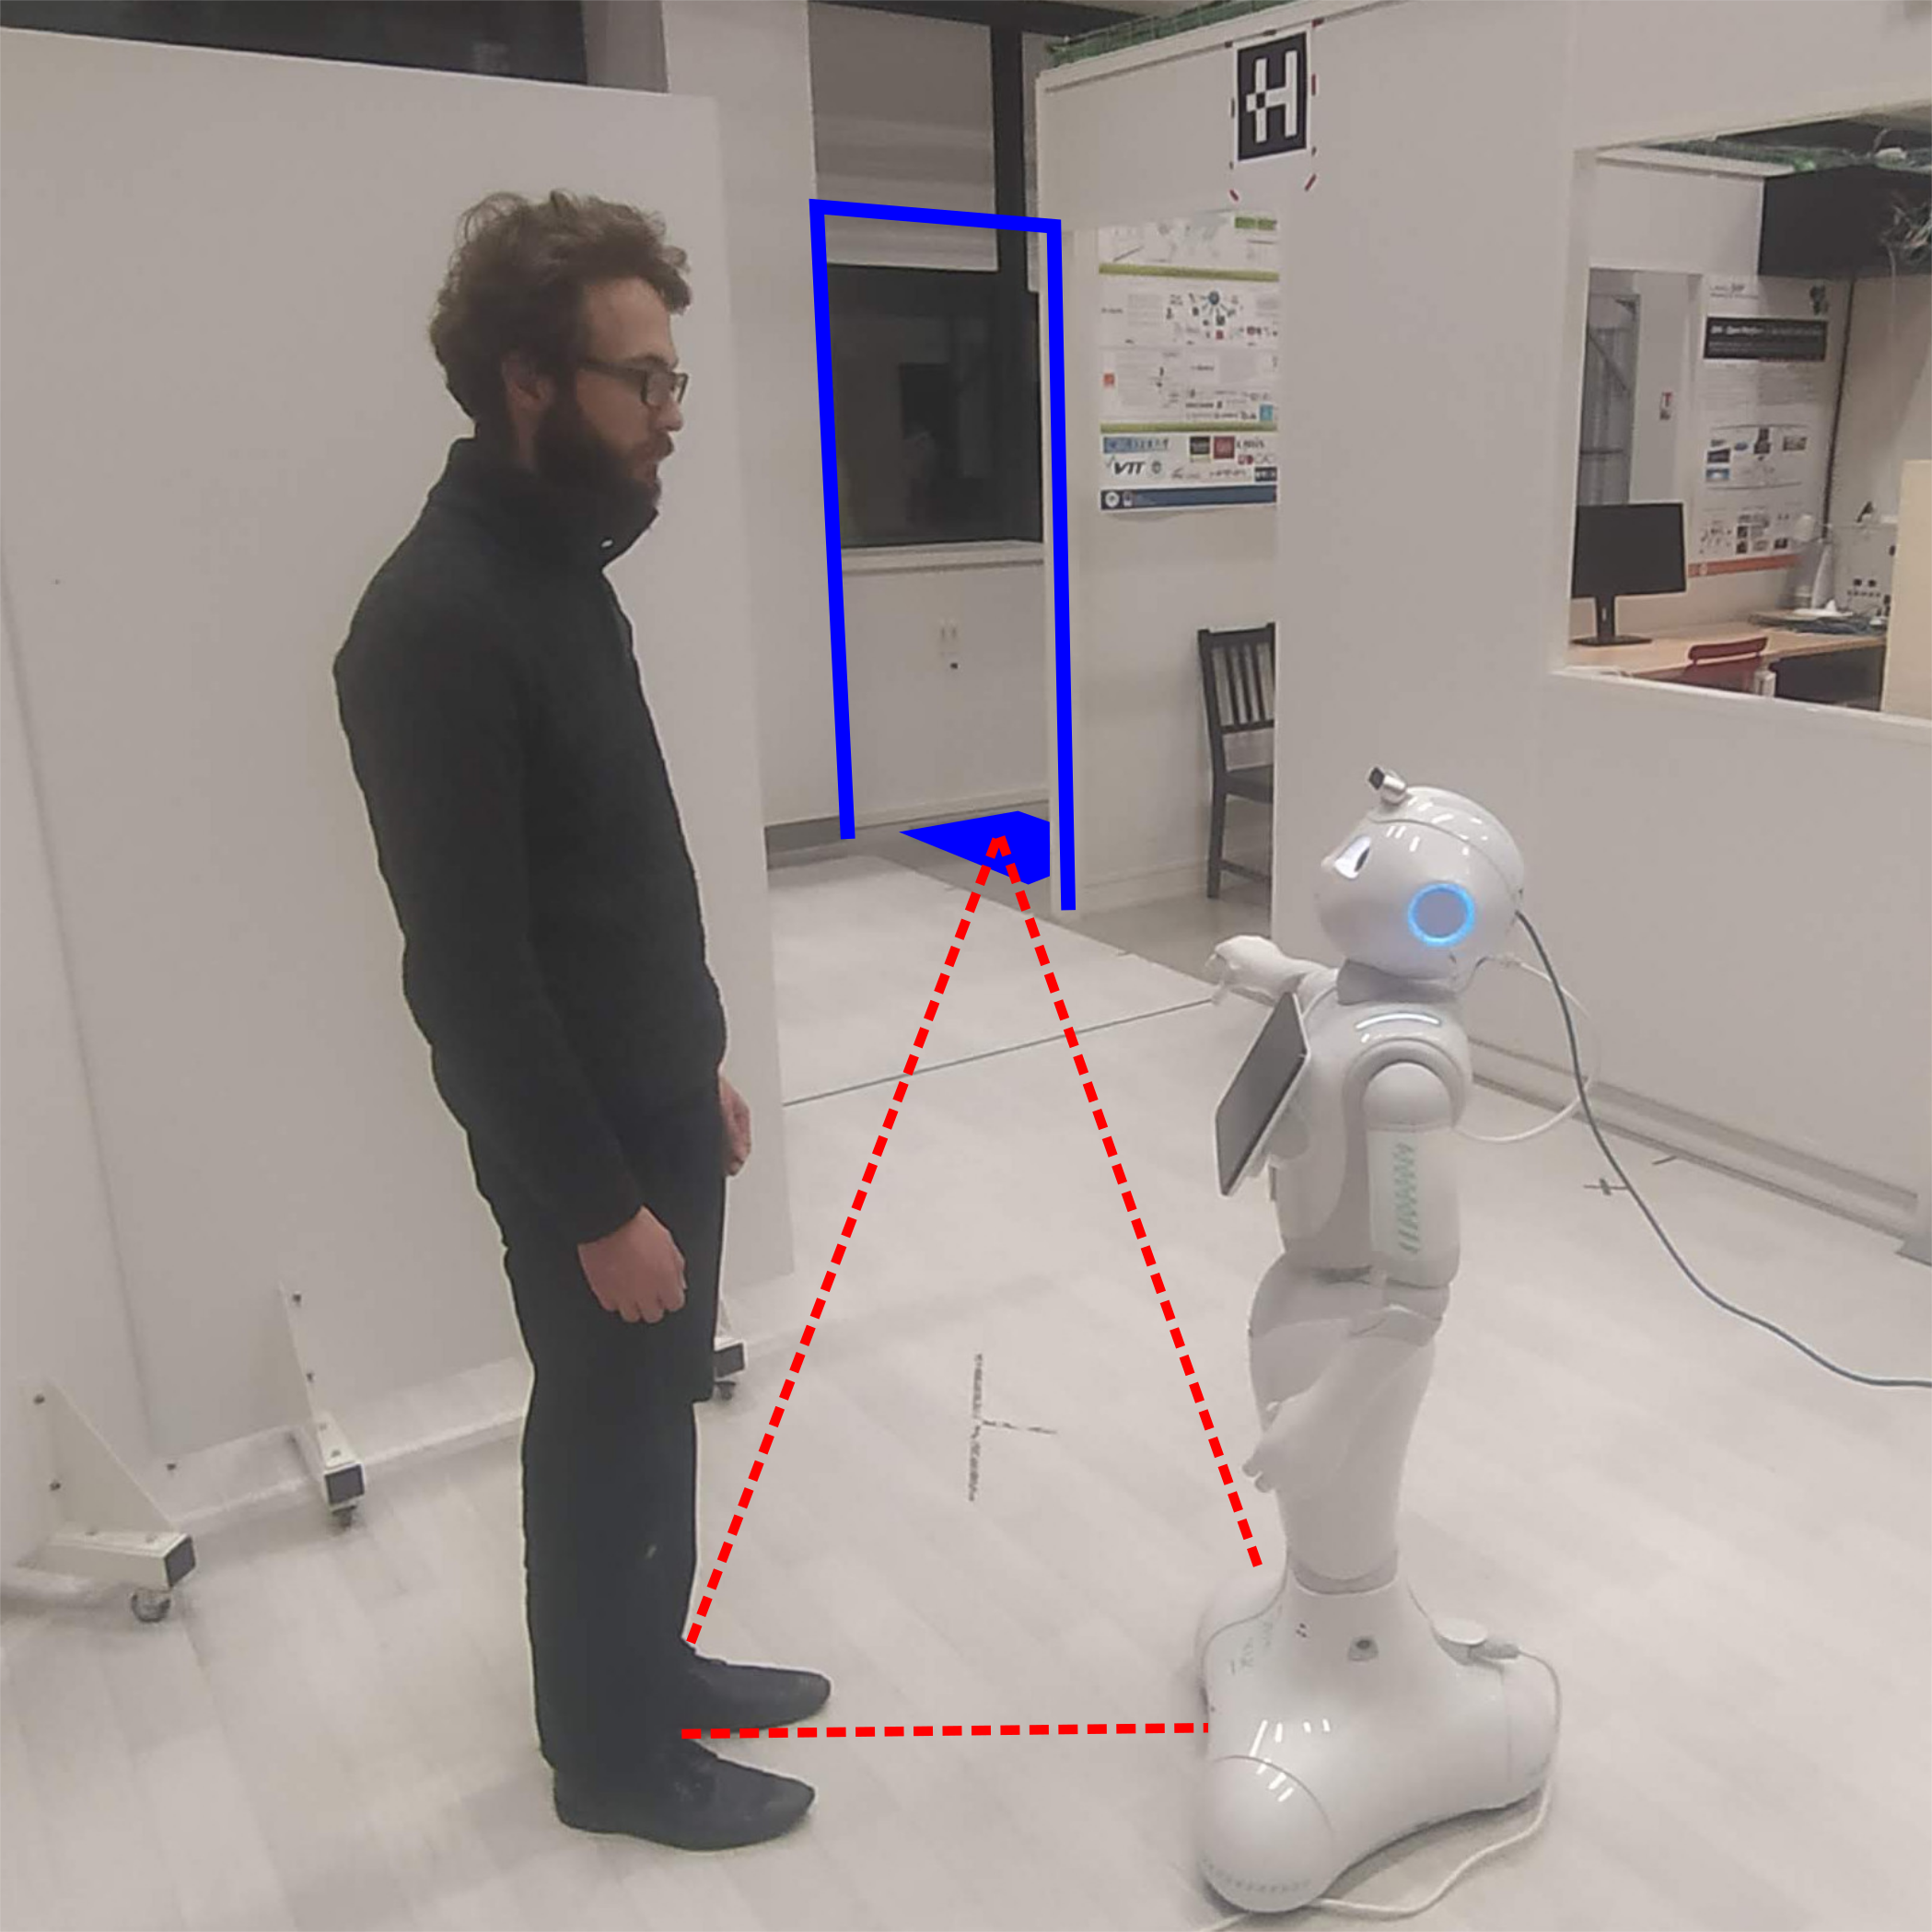
\includegraphics[width=.4\linewidth]{figures/chapter3/final_pose_r.jpg}\hspace{0.1\linewidth}
			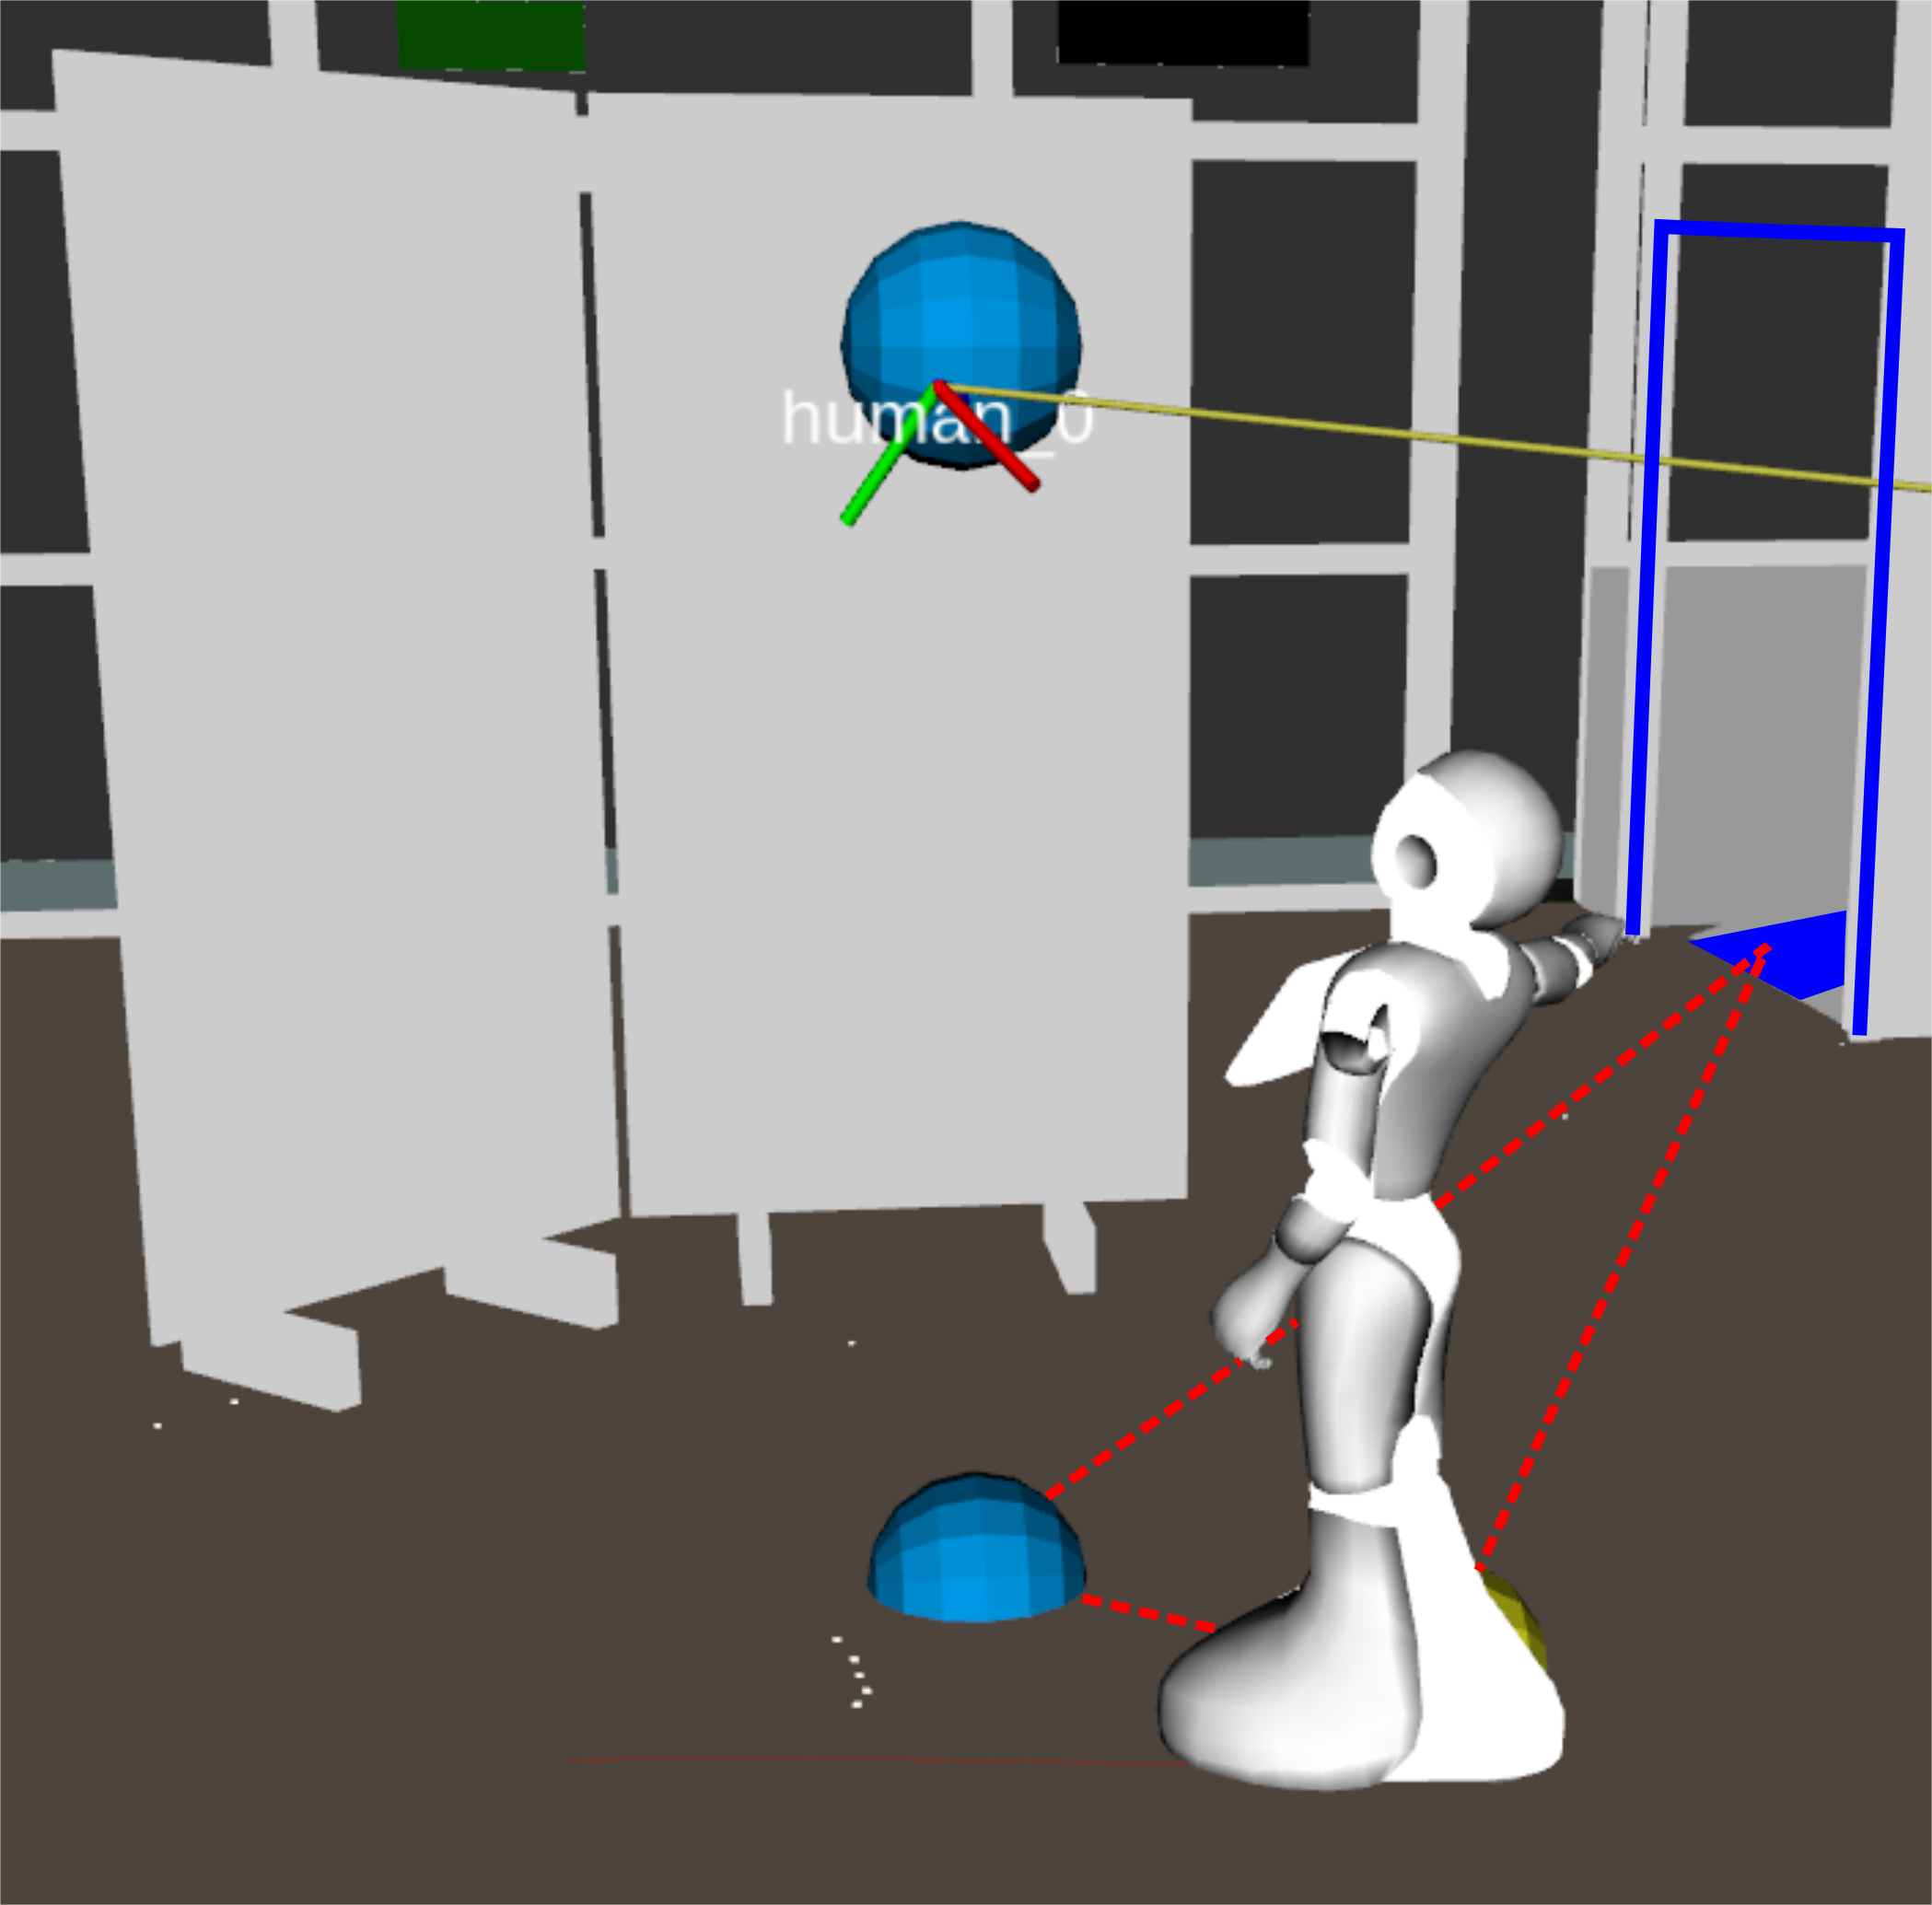
\includegraphics[width=.4\linewidth]{figures/chapter3/final_pose.jpg}
		\end{minipage}
	}\par  
	\caption[pos]{Initial and final positions of a direction-giving task in the lab context. On the left are pictures and on the right screenshots of Rviz\footnotemark (a 3D visualization tool for ROS.)}
	\label{fig:chap3_dir_giving_task}
\end{figure}


To endow a robot with the abilities described above, to build a robotic architecture embedding all these aspects, is a challenge. We tackled it with the architecture presented in the next section.

\section{Description of deliberative architecture}\label{sec:globalarchi}

In this section, we present the robotic architecture developed to handle the direction-giving task. It can be seen as an instantiation of the architecture presented in Section~\ref{chap3:sec:rob_archi}.  

\begin{figure}[ht!]
	\centering
	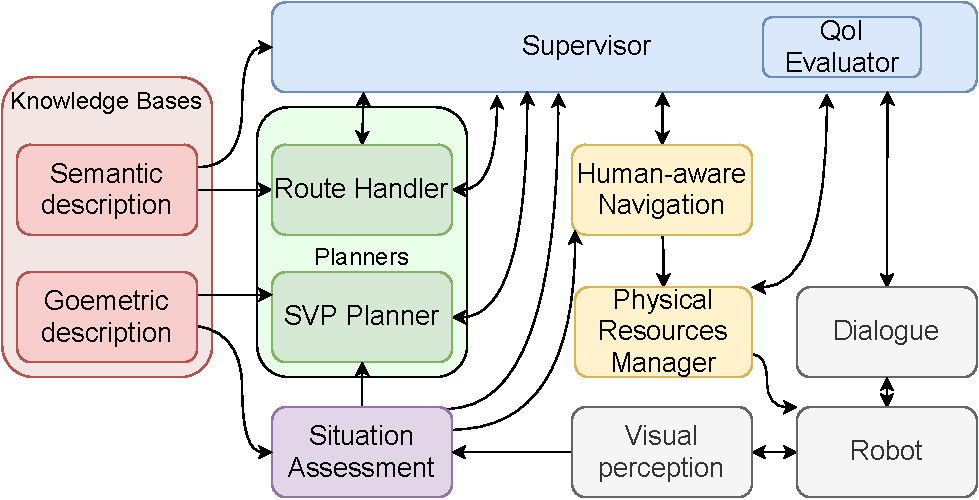
\includegraphics[width=\textwidth]{figures/chapter3/schema_archi.pdf}
	\caption{\label{fig:chap3_architecture} The general architecture of the system. The components presented in this chapter are the colorful ones. The grey ones are from other teams. The visual perception and dialogue components have been respectively developed by IDIAP and HWU and are described in~\cite{foster_2019_mummer}. Naoqi is a Softbank Robotics software.}
\end{figure}

The figure~\ref{fig:chap3_architecture} represents the architecture, its components, and their interconnections. Communication between components relies on ROS. In this chapter, we only present the components developed by the LAAS-RIS team, represented by the colored blocks on the architecture. First, we present the two knowledge representations in the form of geometric and semantic representations. Next, we introduce the components related to the sensorimotor layer: the situation assessment and the physical resource manager. Then, we present the components related to the deliberative layer. They are the Human-Aware Navigation, the SVP (Shared Visual Perspective) planner, the Route Handler, and among the key components, we finish with the supervision and control system, designed to operate human-robot joint tasks in a joint action context. 

\subsection{Environment representation}\label{subsec:models}

For a service robot providing directions to people, we need information to understand humans' need, information to compute the route to the goal, and information to compute the visibility of both agents to plan the pointing position. To understand the needs of a human wanted to be guided, we need information about the type of stores and the sold items. To provide so, Satake \etal{} used an ontology~\cite{satake_2015_field, satake_2015_should}. To compute the route to the final destination, some work show the use a topological map~\cite{matsumoto_2012_you,okuno_2009_providing}. Each node of the graph is related to a 2D position of the environment. To estimate the human visibility of elements anywhere in the environment,  Matsumoto \etal{} used a simplified 3D model where shops are represented by 3D polygons~\cite{matsumoto_2012_you}. In our implementation, we only used two types of representation of the environment: a \textbf{geometric} and a \textbf{semantic}.

Since the final deployment of the robot was in a Finland mall, we have built a mockup mall in our lab for development purposes. By mockup, we mean that shops signs have been displayed in the laboratory to create configuration similar to the real mall. The representations describe hereafter have thus been created both for the real mall and the mockup one.

\subsubsection{Geometric representation}

The geometric representation is used to compute the visibility of elements of the environment from different positions needed for the pointing of landmarks. However, because the robot does not accompany the person to the final destination and therefore does not move much, the possible visibility of the two agents is limited to their immediate environment. For this reason and due to the large scale of the Finland mall, we chose to geometrically describe only the subpart of the global environment that could be visible from the interaction area. For the rest of the environment, we represented the shops with 3D points only. These points are enough to point in the right direction. The resulting geometrical representation is a three-dimensional mesh model, as shown in figure.~\ref{fig:chap3_lab} for the mockup mall and in figure~\ref{fig:chap3_ideapark} for the real one. We have represented in the 3D model all the elements that could hinder visibility, such as poles or panels. In this way, we can precisely emulate human visibility. The model was created from the architectural plans first and then refined with measurements in the mall.

\begin{figure}[!ht]
	\centering
	\begin{subfloat}[The 3D mesh model of the mockup mall at laboratory. The red square represent the interaction area as a square of 4 meters per 4 meters. Signs representing the shops have been place all around the environment.\label{fig:chap3_lab}]{
				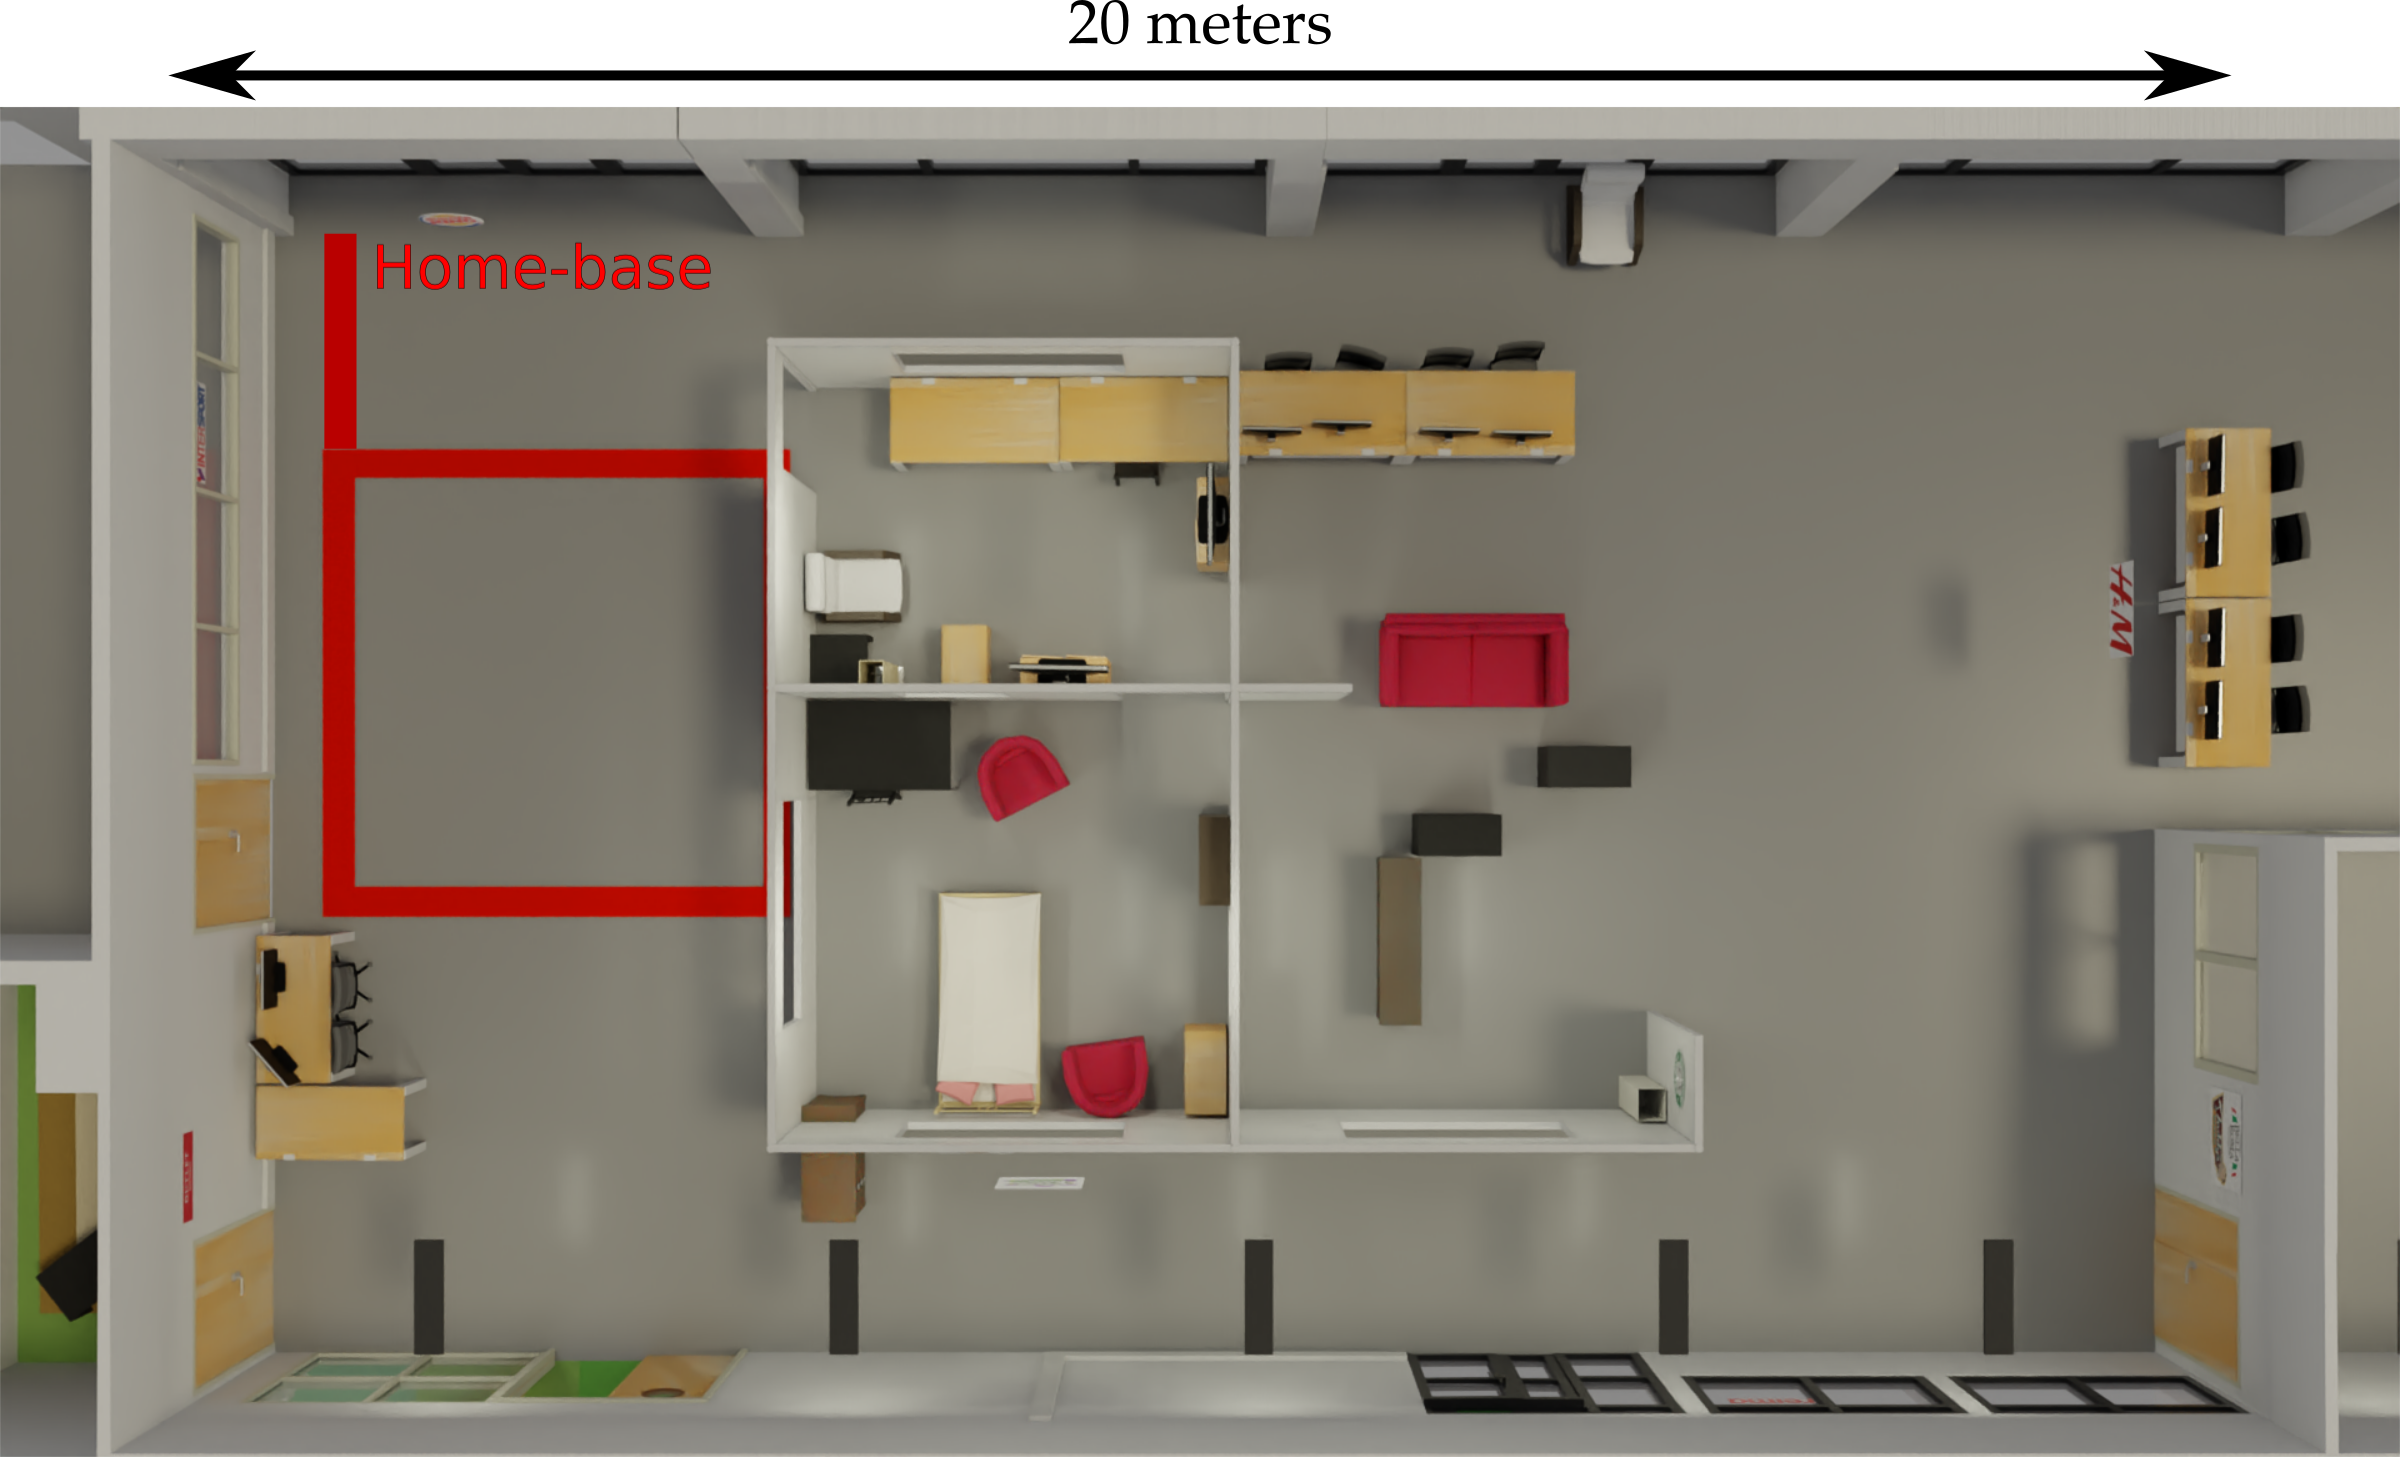
\includegraphics[scale=0.15]{figures/chapter3/adream_base_m.png}}
	\end{subfloat}
	\begin{subfloat}[The 3D mesh model of the real mall in Finland. The entire mall having a size of 528.6 meters per 247.5 meters on two levels, we have only modelled the part which can be visible from the interaction area. It results in a model of 150 meters per 69 meters.\label{fig:chap3_ideapark}]{
			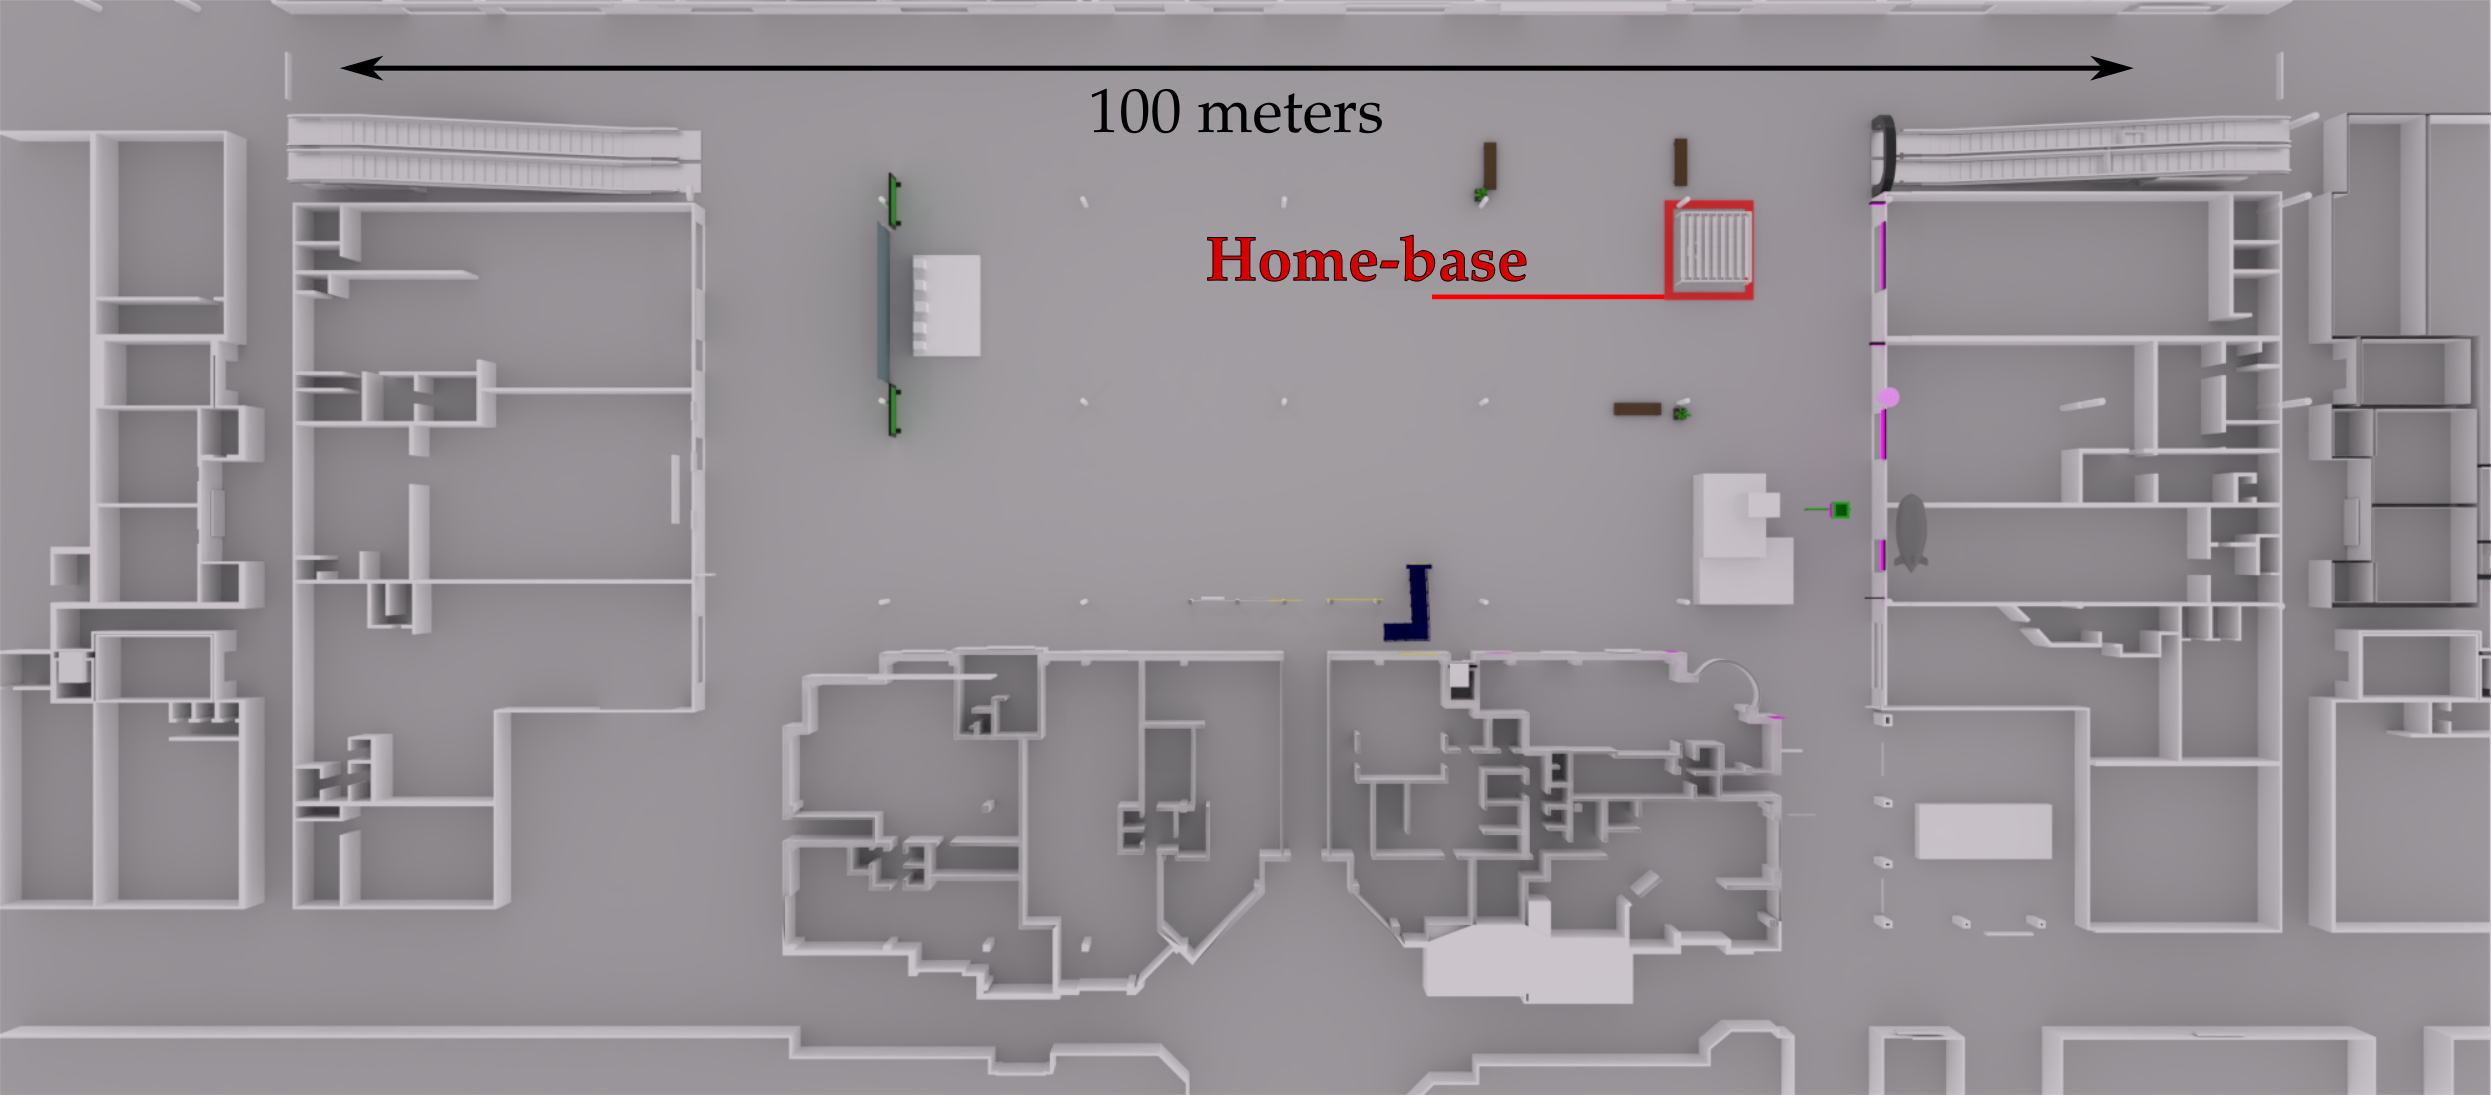
\includegraphics[scale=0.15]{figures/chapter3/ideapark_base_m.png}}
	\end{subfloat}
	\caption{We have built a mockup of the Finnish mall environment in our lab in order to be able to test and debug the direction-giving task in our lab. This environment comprises a two-level area with corridors, ``shops'' , passages, stairs, open central space and consequently allowed us to run realistic guiding scenarios.}
	\label{fig:chap3_3Dmodels}
\end{figure} 


In order for the SVP planner to compute the visibility of the landmarks used for the route description, stairs, escalators, elevators, and store signs are represented each by a single mesh while the rest of the building is a unique 3D mesh. This means that a store is said to be visible if we can see its sign, which we think to be the most relevant element to see to recognize a shop.

The 3D model is also used to generate a navigation map, constraining the robot to move in the interaction area while avoiding obstacles in it.

\subsubsection{Semantic representation}\label{subsubsec:semantic}

As Satake \etal{}~\cite{satake_2015_field}, our semantic representation is based on an ontology. An ontology allows to define classes representing general concepts (\eg Restaurant), individuals/entities being classes instantiations (\eg Burger\_King), and properties linking two entities (\eg Burger\_King isIn Ideapark).
To provide storage and an efficient way to manipulate the ontology and reason about it, a lightweight software has been developed, called Ontologenius, presented by Sarthou \etal{}~\cite{sarthou_2019_ontologenius}. It makes it possible to share the semantic knowledge among all the components of the architecture, here especially the route handler and the supervision, thus enabling a unique repository of knowledge.

As presented in Chapter~\ref{chapter:chap3}, our semantic representation is based on ontology and is stored using Ontologenius. First, it used to represent information about the stores. It allows to define and refine the shared goal of the task by understanding the client's wanted destination. Thus, the stores' types, their names, and the items they sell have been represented in it with a rich semantic. It allows for example to represent that both soda and hamburgers are sold in fast-foods, which are types of restaurants, but that soda can also be found in a supermarket. Thanks to Ontologenius, the names of concepts are defined in different languages and with synonyms for these names. It allows the robot to adapt itself to the human partner language. Moreover, Ontologenius endows the robot with the ability to recognize a set of names in natural language but that it will be prevented to use when itself speaking (\eg the robot can understand a reference to ``bank'' when a human says it but only refers to it as ``ATM'' or ``cash machine'' since there was no bank office in the mall). In addition, this software offers a fuzzy match service based on Levenshtein distance, to help the supervision system to handle ambiguities coming from the speech to text component (\eg it can match the word ``Juwelsport'' with ``Juvesport''). This set of functionalities around the concepts' names facilitates the understanding of the partner's need and thus helps at increasing the quality of interaction.

To include topological information into the semantic representation, the \acrfull{ssr} has been designed, presented by Sarthou \etal{}~\cite{sarthou_2019_semantic}. With the \acrshort{ssr}, the overall knowledge is represented in an ontology with three upper classes which are: \textbf{region} (\ie a two-dimensional area that is a subset of the overall environment), \textbf{path} (\ie a one-dimensional element along which it is possible to move and which has a direction) and \textbf{place} (\ie a point of zero dimension that can represent a physical or symbolic element). The \textbf{place} class has three subclasses: \textbf{path intersection} (\ie the connection between only two paths and thus a waypoint to go from one path to another), \textbf{passage} (\ie the connection between only two regions and thus a waypoint to move from one region to another like a door, a staircase or a passage), and \textbf{shops}. A representation of these classes is visible in Figure~\ref{fig:chap3_onto_classes}.

\begin{figure}[!ht]
	\centering
	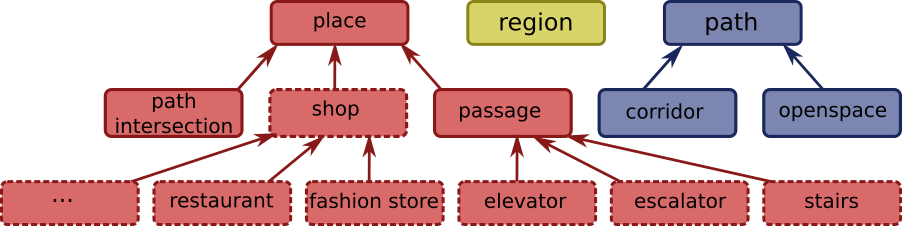
\includegraphics[scale=0.45]{figures/chapter3/classes.png}
	\caption{\label{fig:chap3_onto_classes} Classes for a representation of the topology of an indoor environment in a semantic description. The classes with the solid outline are the minimum classes defined by the \acrshort{ssr}. The classes with the dotted outline are an extension of this minimal set.}
\end{figure}

An example of the final semantic knowledge represented in the ontology for a given shop is presented in Figure~\ref{fig:chap3_onto_properties}. We find here the identifier of the shop, the category to which each store belongs (\eg restaurant or hairdresser), the items sold for which people ask the most (\eg shoes or coat), and the names and synonyms in natural language and that for different languages.
Moreover, thanks to the \acrshort{ssr} we can produce the best route (in term of complexity) as well as verbalize it using a route perspective.

\begin{figure}[!ht]
	\centering
	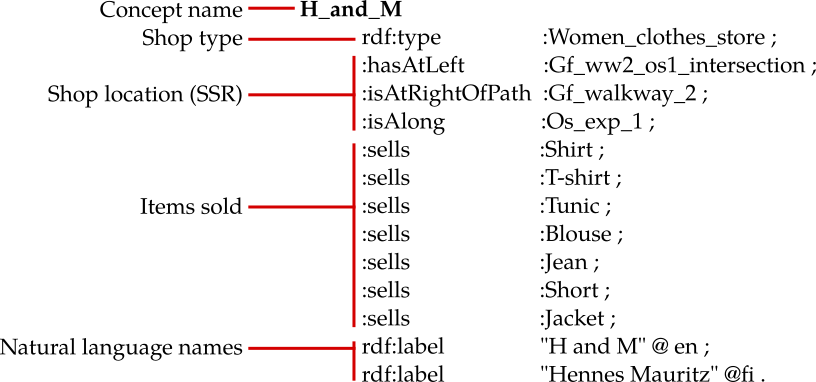
\includegraphics[scale=0.45]{figures/chapter3/zizzi.png}
	\caption{\label{fig:chap3_onto_properties} Properties for a representation of the topology of an indoor environment in a semantic description.}
\end{figure}

\subsection{Perceiving the partner}\label{subsec:situation_assessment}

The situation assessment component is based on the Underworld framework~\cite{lemaignan_2018_underworlds}. It aims at gathering perception information in the form of 3D position and orientation of human faces, with the 3D model and the robot state. With this information, it is able to generate the symbolics facts listed in table~\ref{tab:chap3_predicates}.

\begin{table}[ht!]
	\centering
	\begin{tabularx}{\textwidth}{|l|X|}
		\hline
		\textbf{Predicate} & \textbf{Description} \\
		\hline
		\hline
		isPerceiving & The robot is perceiving a human \\
		\hline
		isCloseTo & The human is within a distance of 0 to 1 meter of the robot \\
		\hline
		isLookingAt & The human is looking at the robot \\
		\hline
		\hline
		isInArea & The human is in the interaction area \\
		\hline
		isEngagingWith & The human is close to the robot and is looking at it \\
		\hline
	\end{tabularx}
	\caption{Facts computed and monitored during the direction-giving task.}
	\label{tab:chap3_predicates}
\end{table}

\subsection{Managing the robot's resources}

A humanoid robot such as Pepper can be seen as a composition of multiple physical components that can act independently of each other. For the direction-giving task, we identified four resources: the head, both arms, and the base. At the beginning of the interaction, for example, the head is used to find people to interact with, but later it will be used to track the human with the gaze. Several components could access this resource to perform these actions. However, they do not have a global picture of the ongoing task. In this case, a resource could be used by several components at the time. Consequently, it could lead to task failures.

Moreover, in some cases, several resources have to be used simultaneously to perform a high-level action. To point to a landmark, one arm is selected to point while the other has to be lowered. The base is then rotated if the arm reaches the joint limit to point a target on its back. If at least one of the involved resources is simultaneously used to perform another action, the overall high-level action will fail as the global posture will no more be clear. For example, if the human gets too close to the robot and a component tries to move away from a little, the arm would no more point in the right direction.

Thus, for each of the identified resources we instantiated a Resource Manager that we presented in Section~\ref{chap6:para:resource_m}. The global resource management scheme is illustrated in Figure~\ref{fig:chap3_rm} with four resource managers and one synchronizer.

\begin{figure}[!hb]
	\centering
	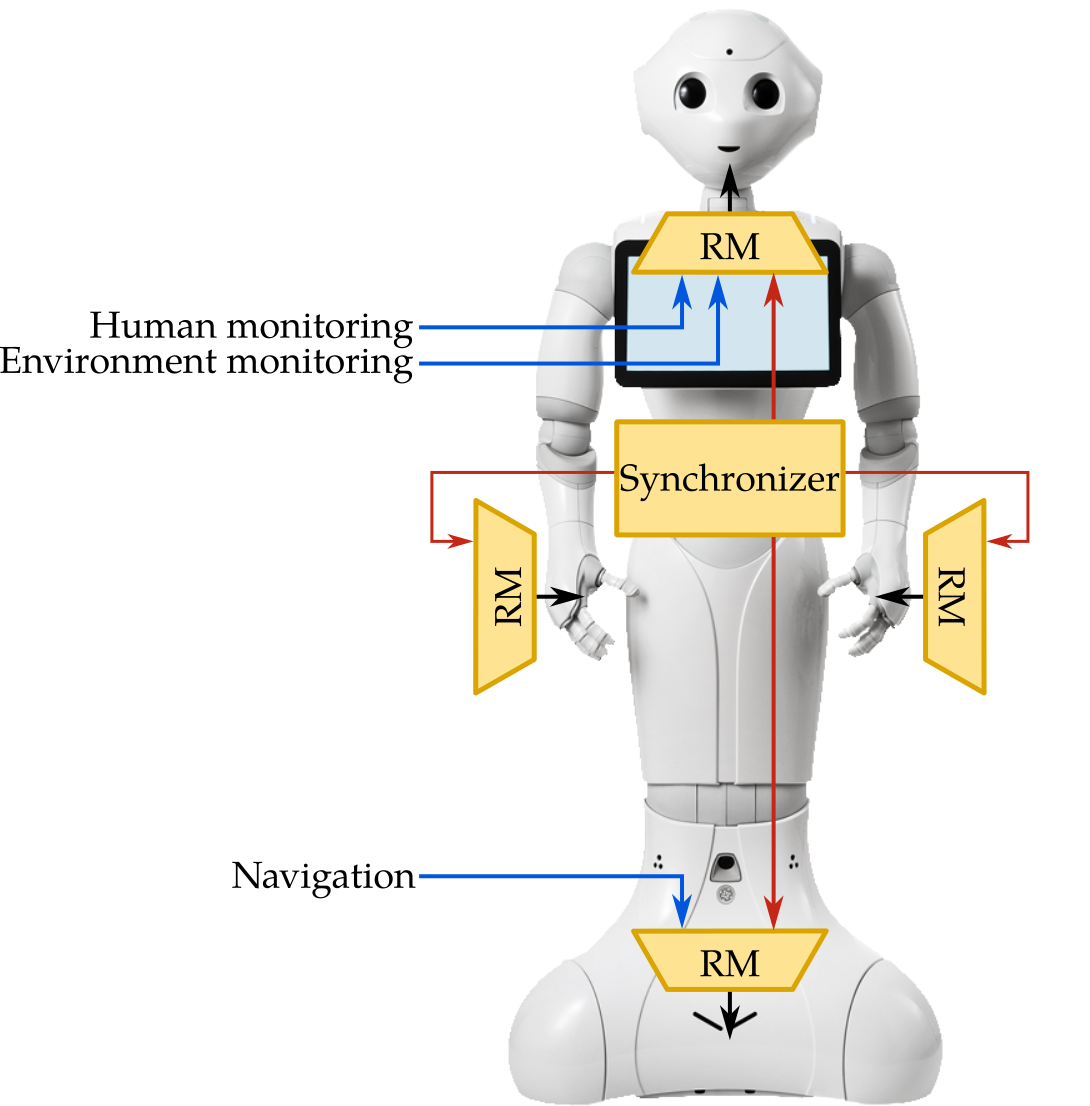
\includegraphics[scale=0.26]{figures/chapter3/rm.png}
	\caption{\label{fig:chap3_rm} Representation of the resource management system with four resource managers and a synchronizer. The red arrows represent the state machines inputs and the blue arrows represent the inputs for permanent commands.}
\end{figure}

\subsection{Describing the route to follow}\label{subsec:route_description}

Algorithms have been specifically developed in the context of this project in order to find the best route(s) to go from one place to the other in an environment with ``places'' (\eg shops, toilets, stairs), and ``paths'' (\eg corridors). These algorithms are presented in~\cite{sarthou_2019_semantic}. 

The dedicated component receives requests with:
\begin{inlineEnumerate}
	\item the departure place,
	\item the goal place, and
	\item an option to specify some constraints (\eg no stairs).
\end{inlineEnumerate}

It outputs a set of routes, with a route being of the form $place - path - place - ... - place$, and a cost associated to each of these routes. 

The second place of the route -- the third element of the route objects -- is the one we call the passage in the description of the direction-giving task, the first salient landmark of the route to point to, which is on the way to reach the final place. For example, the best route to go to the restaurant Bella Roma from the robot base is: [``pepper\_infodesk'',``Keskuspuisto'',``escalator\_sauruskatu'',``corridor\_1food'',\\``Bella\_Roma''], with ``pepper\_infodesk'' the departure place, ``escalator\_sauruskatu'' the passage and ``Bella\_Roma'' the goal place.


\subsection{Planning a shared visual perspective}\label{subsec:svp}

When the robot has to point to a target, two criteria have to be respected. First, the human has to be able to see the target. Second, the human has to be able to look at the pointed target and at the robot without turning the head too much. It goes the same for the robot as it has to see the pointed target, meaning not to point toward a wall and be able to simultaneously point at the target and look at the human. Consequently, to point a target in its back, it has to move. The robot and the human can thus move in the interaction area during the direction-giving task, to move to a better position for pointing at the target. To find the robot and human possible positions we designed a component called the SVP (Shared Visual Perspective) Planner, presented in~\cite{waldhart_2019_reasoning}. For the purpose of the deployment, the presented version is an adapted and slightly simplified version.

To compute the visibility of both agents, the planner has access to the geometrical representation of the environment and the agents current positions. In addition, it considers an estimated agent's maximal speed to move and a visibility threshold.

When the robot explains the route to the human and points to a landmark, they form what is called an F-formation. Kendon explains that \emph{``An F-formation arises whenever two or more people sustain a spatial and orientational relationship in which the space between them is one to which they have equal, direct and exclusive access''} ~\cite{kendon_1990_conducting}.
This F-formation has been decomposed by McNeill into two types: the social formation and the instrumental formation~\cite{mcneill_2005_gesture}. While the first type corresponds to the original definition, the instrumental formation includes a physical object that all the agents can gaze at. This means that once the robot will have moved, the human will come in front of it creating a social formation in the form of a vis-a-vis (each facing the other) and when the robot will point they will change for an instrumental formation. Indeed, when both agents will reach their position computed by the planner, we want them to be able to go from one formation to the other with only a rotation; the human will not need to move again from their arriving position to see what the robot will point. 

To search for better positions to reach in order to point a landmark, the planner takes three main parameters into account:

\begin{bulletList}
	\item Visibility constraint: The two agents can see either the target shop when it is the only element of the route or the passage.
	\item Navigation distance cost: The agents do not have to move too much.
	\item F-formation cost: The human-robot-target angle and a robot-human-target have to be less than 90${^\circ}$. 
\end{bulletList}

\begin{figure}[ht!]
	\centering
	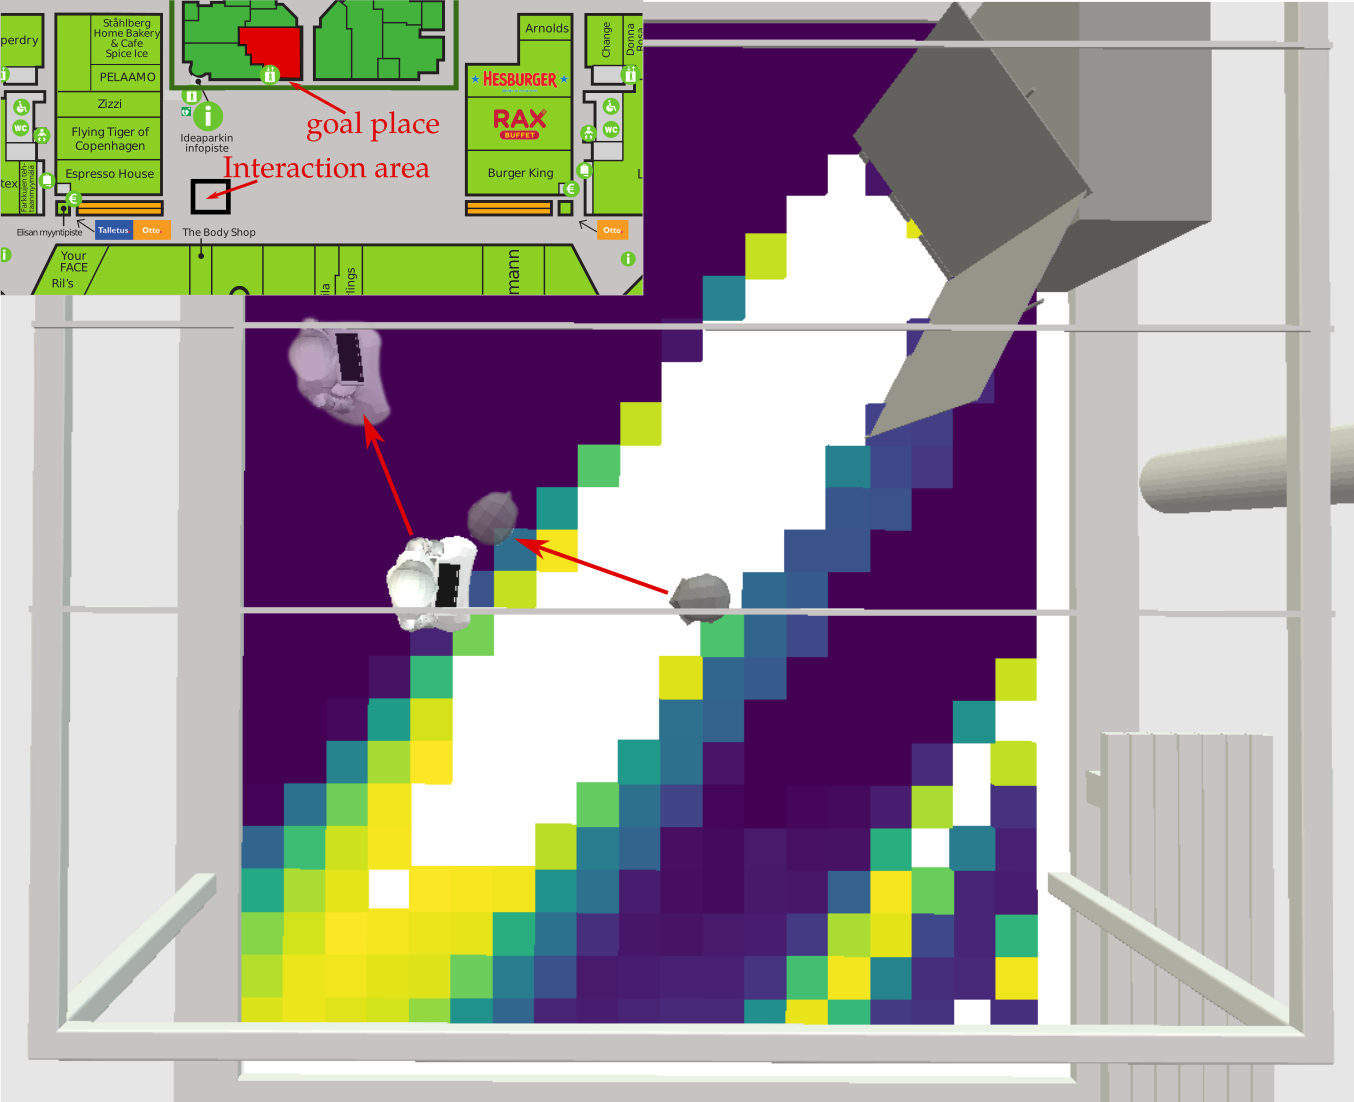
\includegraphics[scale=0.3]{figures/chapter3/grid_map.png}
	\caption{\label{fig:chap3_svp_grid} Visibility grid for a target located at the top right. The uncoloured areas represent an absence of visibility and the others represent the cost of visibility ranging from yellow for low visibility to purple for good visibility. The robot and the human in transparency on the image represent the final calculated positions while the others are the initial positions. }
\end{figure}

To compute the positions, the interaction area is firstly decomposed into a weighted three-dimensional (x,y for the possible positions in the area and z for the human height) grid representing the estimated human visibility of the target. The target visibility is computed offline for each position of the grid. It is based on the part that the target takes in the 360${^\circ}$ field of view of the environment. Such grid is represented in figure~\ref{fig:chap3_svp_grid} for a given human height. The white cells are positions from which the human cannot see the pointed target. The other colored cells represent the degree of visibility from the poor in yellow to the good in purple. Having the human visibility grid, the goal position is computed using a weighted cost function between good visibility and restricted distance to cross. In the example of figure~\ref{fig:chap3_svp_grid}, the transparent human head is the human goal position while the other is the initial position. From the initial position, the human was not able to the pointed target. 

The robot position is computed in a second time, according to the human planned position. Divided the search into two steps allows reducing the search complexity. The robot position is thus constrained by the human one. It has also to respect a minimal and maximal distance to the human and minimal visibility of the target from it. Finally, the robot position is also determined regarding a cost preferring an F-formation limiting the robot reorientation, meaning that it can point to the target keeping its torso and its chest oriented towards the human.


\subsection{Navigate close to human}\label{subsec:navigation}

The Human-Aware Navigation component aims at moving the robot while avoiding dynamic and static obstacles in addition to proposing a socially acceptable navigation solution for the robot. For example, the robot should not pass too close to the human and should not show its back while navigating around the human. A full presentation of the planner is available in~\cite{singamaneni_2020_hateb}.

\subsection{Robot execution control and supervision in a joint action context}\label{subsec:supervision}

The work presented about the supervision in this section is an early version of \acrfull{jahrvis} presented in Chapters~\ref{chapter:chap5} and~\ref{chapter:chap6}. It integrates on one hand the decision and control for the direction-giving task, and on the other hand the implementation in this task context of the metrics presented in Chapter~\ref{chapter:chap7}, to measure the Quality of Interaction.

\subsubsection{A supervision and control system dedicated to human-robot joint tasks}
A service robot interacting with humans in a mall and providing directions to them needs a number of abilities to enable a smooth and efficient interaction. As explained in Section~\ref{sec:rationale}, the direction giving task is an asymmetric joint action, with the robot in the guide role and the human in the guided role. The Supervisor is built taking this specificity into account, embedding a shared representation of the direction giving task. More specifically, when giving directions to a human, the robot plans its actions and the human ones and then executes its part of the plan. To be able to know if and when the human performs their actions, it monitors the execution of actions and interprets the information directly received from the Situation Assessment (see Section~\ref{subsec:situation_assessment}). Furthermore, in such interaction, communication is important, thus the robot communicates verbally as well as non-verbally, and listens to the human. All along the interaction, it needs to maintain a distinct mental state model for the human and itself concerning the knowledge of both agents and the state of the world. Finally, it should be able to tackle events and contingencies happening during the task and to drop it when necessary.

During an interaction session (see Section~\ref{chap5:sec:levels}), \emph{direction-giving task} occurs when the human involved in the ongoing interaction session  asks for directions to a place or for locations of sold items. 
% The robot, if necessary, refines the human goal, establishes a shared goal~\cite{cohen1991}, enquires about their willingness and abilities of climbing stairs, updates its estimation of the human mental state. Then, it gives route directions while pointing at landmarks, taking their perspective into account for the landmark and the route. Finally, it checks if it has been understood, making sure that the person has all the information to complete the shared goal, being the human reaching its destination. The robot executes all these steps thanks to \emph{actions}, communicative ones or on the environment.


\subsubsection{Implementation of the direction-giving task and its associated actions}\label{subsubsec:sup:subtasks}
\begin{figure}[hbtp]
	\centering
	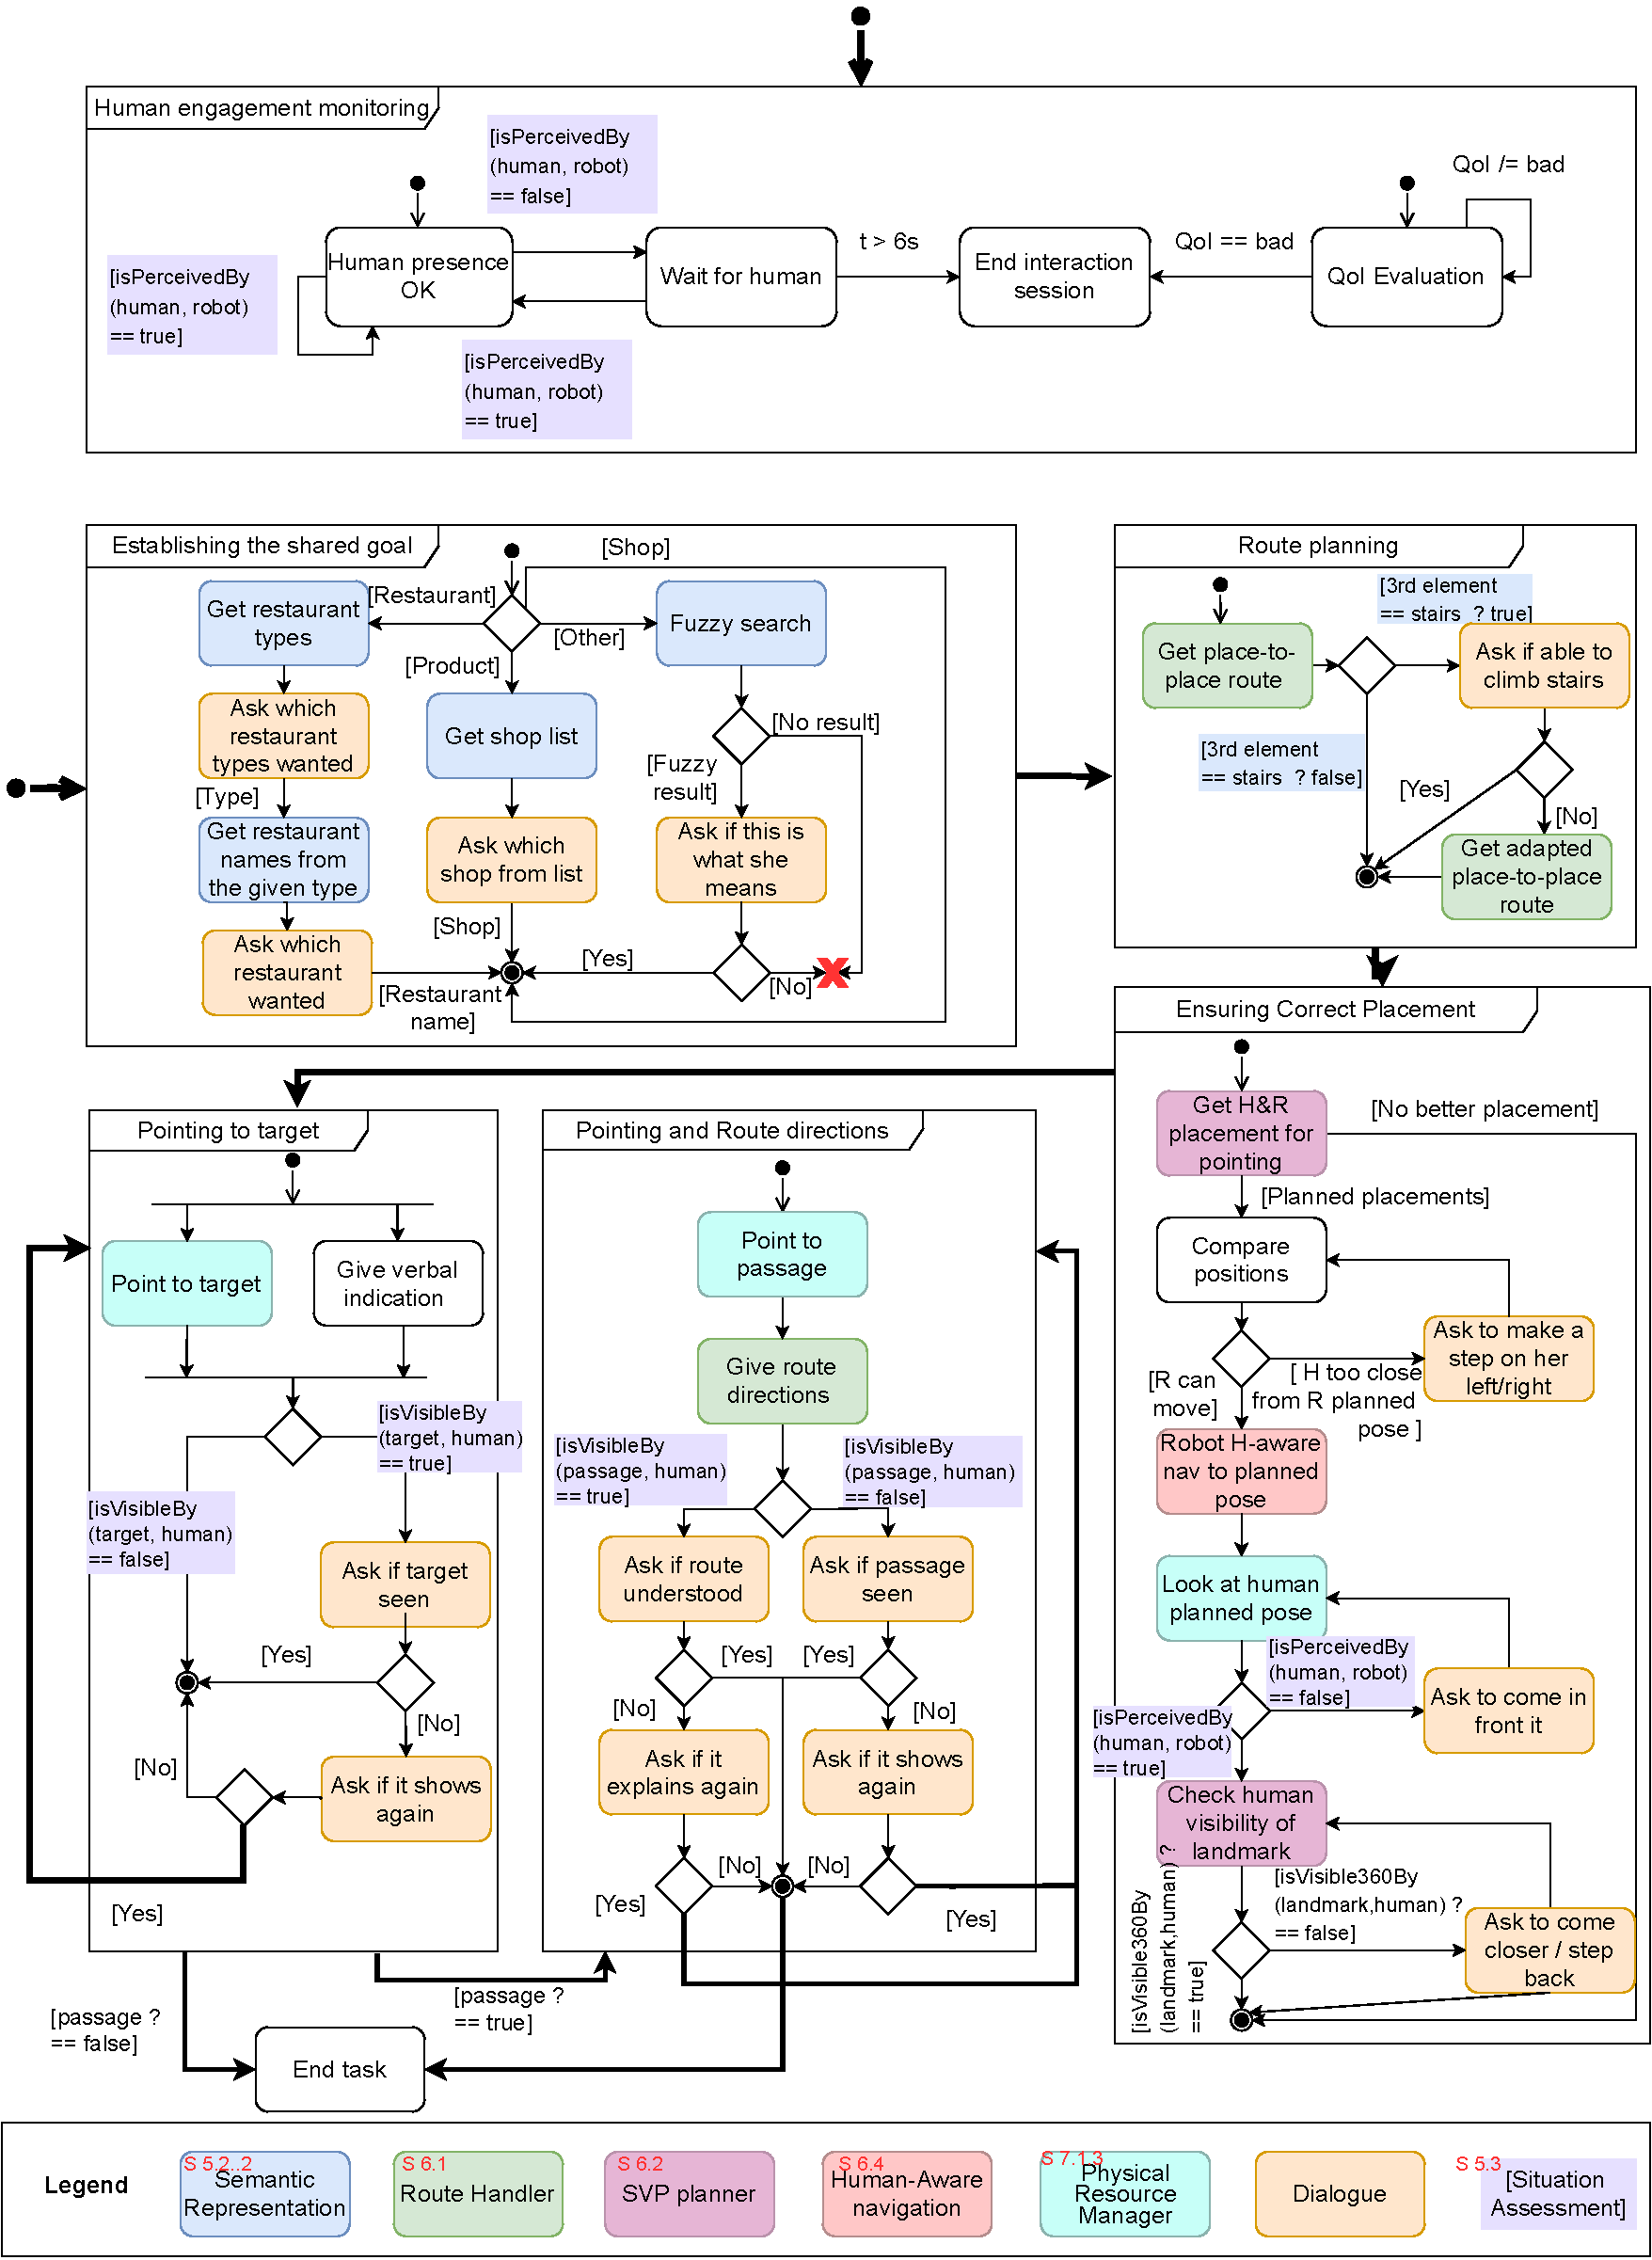
\includegraphics[width=\linewidth]{figures/chapter3/state_machines.pdf}
	\caption{\label{fig:chap3_SM} Supervisor activity diagram of the direction-giving task. Each action has a color corresponding to the component with which the Supervisor interacts to execute it. It goes through every subtasks described in Section~\ref{subsubsec:sup:subtasks}. Also, the human engagement monitoring is represented. Texts between brackets correspond to beliefs on which depends the decision-making process. These beliefs can either be provided by other components or being the result of the Supervisor's own computations. }
\end{figure}


In the direction-giving task, plans were not computed by a planner as presented in Chapter~\ref{chapter:chap6} but were written with Jason reactive plans (see Section~\ref{chap4:subsec:jason}). Thus, at execution time, the Supervisor does not handle one shared plan received from a planner but plenty of (reactive) plans which are chosen among the ones from the plan library when triggered by an event or by another plan. The same plan can have multiple versions and the version to be executed is selected according to the pre-conditions (also called context). For instance, the plan \textit{verbalization(Target)} has two different versions, one in the case where the target to point is visible and the other one in the case where it is not, and at execution time, the selected one will depend on the presence or not of the belief \texttt{visible\_target(Target)} in the Supervisor belief base, as shown in Listing \ref{listing:plan}:

\begin{lstlisting}[caption = Two different plans for \texttt{verbalization(Target)}, label = {listing:plan}]
+!verbalization(Target)                 // plan name
: visible_target(Target)            // context
<-  ?verba_name(Target, Name);      // belief query
say(visible_target(Name)).      // action

+!verbalization(Target) 
: not visible_target(Target)
<-  ?verba_name(Target, Name);
say(not_visible_target(Name)).
\end{lstlisting}

Even though the direction-giving task is implemented with reactive plans, it can still be represented with an activity diagram, for presentation purposes. This activity diagram is visible in Figure~\ref{fig:chap3_SM}. Each frame represents one of the steps described in Section~\ref{sec:guiding}. We now present their internal functioning and the interactions with the multiple components of the system the Supervisor has.

\paragraph{Establishing the shared goal}
When a person triggers a direction-giving task, they might directly ask something like ``where is the pharmacy?'' which allows the robot to directly establish the shared goal but, they might also ask something less precise. In the latter case, the robot needs to inquire about the human desired place to reach in order to establish the shared goal.

When a person asks ``Where is a good restaurant?'', the robot presents a list of the types of food available, namely ``There are casual dining restaurants, Asian restaurants, native food restaurants, hamburger restaurants, fast food restaurants, and pizzerias.''. This behavior is quite similar to the recommendation behaviors of Kanda \etal{}~\cite{kanda_2009_affective}.

To be able to display this behavior, several components of the system are requested. When the Supervisor receives $\{request=restaurant\}$ as data from the Dialogue, it asks Ontologenius for all the existing restaurant types. This list of restaurant types is sent to the Dialogue whose role is to return to the Supervisor with the type selected by the human. Finally, similarly to the way it obtained the restaurant type from the human, the Supervisor tries to get the restaurant name. Therefore, it requests from Ontologenius all the restaurants serving the given type of food. Then, this list is sent to the Dialogue whose role is to return to the Supervisor with the restaurant selected by the human among the elements' list. It should be noted that all the restaurants of the given type are suggested to the person, even though sometimes the list is long. We thought of alternatives such as randomly giving three restaurants among the ones of the list. However, these alternatives were not allowed by the mall policy as they could not provide equality between all shops. 

The same principle goes for products. For example, people can ask ``Where can I buy a dress?''. Then, the Supervisor gets from Ontologenius a list of shops selling dresses and passes it to the Dialogue. The Dialogue returns the name of the shop chosen by the person.

When the Supervisor receives as a goal a name it does not understand, it queries Ontologenius to try to match it to a known name as it may be not understood because of a speech recognition failure or a shortened name. For instance, thanks to the fuzzy match provided by Ontologenius, when a person asks to go to ``jewelsport'', the system can make the assumption that the person actually asked for ``Juvesport''. So the robot asks the person, ``do you mean Juvesport?'', to which the person can answer ``yes'' or ``no''. If yes, it starts the direction-giving task, if no it drops it and returns in chat mode.

\paragraph{Enquiry about human willingness and abilities to climb stairs}
As the robot is there to help humans, it has to adapt to their abilities and preferences such as a person with a shopping trolley will prefer to take escalators than stairs. The preferences definition is currently done through verbal communication.

To determine human preferences about stairs, the Supervisor first requests to the Route Handler (see Section~\ref{subsec:route_description}) the possible routes to go to the target shop. The returned routes are of the form $place - path - place - ... - place$. The Supervisor selects the one with the smallest cost and then checks if one of the $place$ elements is stairs (\ie the Supervisor queries Ontologenius for the element type). If it is the case, the Supervisor asks the Dialogue with finding out if the human is able to climb stairs or not. If not, it will send a new request to the Route Handler with the parameter ``no stairs'' and will get a new set of routes. The Supervisor selects the one with the smallest cost. This new route will have a cost equal to or higher than the first one (since it was not the route with the smallest cost in the initial request), which means the goal might be more complicated to reach or it might take more time.

\paragraph{Ensuring a correct placement}
The robot's role in this task is not only to give verbal route directions but also to point to the target and the passage (\ie the third element of the route as explained Section~\ref{subsec:route_description}) the person should take in order to increase the chances that they reach their destination as it helps to orientate them in space. For the pointing to be as efficient as possible, the robot computes new positions for itself and the human where the visibility of the pointed landmarks will be better (when feasible). Then its goal is to have itself and the human reaching these new positions. 

In the first step of this subtask, the Supervisor requests from the Shared Visual Perspective (SVP) Planner (see Section~\ref{subsec:svp}) the new positions for the robot and the human, with the passage to point (or the target if no passage) and the human identifier as parameters. Then, the Supervisor compares the newly received positions with the current ones of the human and the robot -- the current position of the human is provided by the Situation Assessment. In the case where the robot planned position is very close to the human's current position (\textless~0.5~m), the robot asks the human to step aside on the right or left, depending on the human's planned position. If the human does not move or does not go far enough from the planned robot position, the robot will ask again.

Then, the Supervisor requests the Human-Aware Navigation (see Section~\ref{subsec:navigation})  to move the robot to its planned position. Once the Human-Aware Navigation returned that the position has been reached, the Supervisor looks for the human. It is a form of monitoring, which we show in Section~\ref{sec:rationale} is important in a joint action. If the human is not perceived -- the Supervisor did not receive from the Situation Assessment the predicate isPerceiving(\(robot, human_i\)) -- in the following seconds (6 seconds in the deployed version), the robot asks the human to come in front of it -- this is the way we have chosen after several trials (other modalities like indicating to the human by a gesture where they should stand were not sufficiently successful). If the human is still not perceived after a few seconds, the robot will ask again, remaining engaged in their joint action for a while before giving up.

Once the human arrives in the robot field of view -- which means that the human more or less reached their planned position since the robot is looking in the direction of it --, they might not exactly be at their planned position. In this case, their position may not be suited to properly see what the robot has to point at. To check if they are in a position good enough to see, the Supervisor asks the SVP Planner for the visibility (at 360 degrees) of the landmark to point. In the case where the SVP Planner returns that the landmark is visible, the interaction continues. Else, the robot asks the human to move forward or backward in order to adjust their placement according to their planned position. This stops when the robot computes that the position of the human will allow them to see the target. In this way, the robot tries to ensure to put the human in the best conditions as possible for the next steps, using key elements of the joint action: monitoring of the partner actions', sharing a visual perspective and showing engagement in the task.

\paragraph{Pointing to target}
As it is shown that the use of deictic gestures such as pointing improves the understanding of route directions (see Section~\ref{sec:methodology}), we endowed the robot with this ability. 

To do so, the Supervisor requests from the Physical Resource Manager that the robot points to the target. At the same time, it generates a short sentence for the robot to say and sends it to the Dialogue. The sentence varies according to the visibility of the target such as ``Here, you can see Burger King'' for a visible place and ``The restroom is in this direction'' for a non-visible one. In this way, the robot shares the human's perspective and takes into account the knowledge they can get from their environment in respect of the joint action principles. In this way, the human knows if they have to try to notice it from their place or take this information as an orientation indication. In order to continuously look at the human and not loose them from its sight, the robot does not turn its head towards the target when pointing.

It is important for the robot to know if it successfully communicated the information to the human. Then, it asks if the target has been seen, as it wants to ensure its action had the expected effect.

\paragraph{Pointing to passage and giving route directions}\label{par:route_understood}
This step is executed when there is a passage in the route returned by the Route Handler. Therefore, the Supervisor sends a route to the Route Handler which returns a verbalization of this route (\eg ``Walk through that corridor, and then, turn left. From there on, Apteekki will be on your right, straight after Glitter''). Then, as explained in the \emph{Pointing to target} paragraph, the robot points, to the passage this time. And, at the same time, it verbalizes the route received from the Route Handler, added "in this direction" to the sentence if the passage is not visible.

As for ensuring the target has been seen, the robot wants to make sure it has been understood and leaves the possibility to the human to hear the route directions again if they need it. In the early versions, we had programmed the robot to ask if the passage had been seen and then if the route had been understood but it was too many questions that seemed useless to users. Indeed, we analyzed it as a postcompletion error~\cite{byrne_1997}, as the goal of the human was to know the route to their location, whatever actions arising after this goal has been completed are often forgotten. In the end, the first question is asked in case of a visible passage and the second one is asked in case of a non-visible one.

It may be noted in Figure~\ref{fig:chap3_SM} that it is possible to go in infinite loops such as Route directions - Ensuring route understood - Route directions - ... . To avoid this issue, the Supervisor prevents to return inside a step if it has already been executed a certain number of times (in the final version, 3 was the maximal number a step could be executed).

\section{The deliberative architecture in a real-world environment}\label{subsec:archi-integration}

In the previous section, we presented a deliberative architecture designed to be embedded in a service robot. The purpose of this robot was to be deployed in a mall in Finland. 
To make this deployment successful, we did extensive tests in our laboratory where we had reproduced a part of the mall environment to be in the most realistic conditions possible\footnote{This setup not only was used for tests but also for public demos and even in the context of a scientific live event now accessible on \url{https://youtu.be/p4f3iwHht2Q?t=4495}}. Some of these emulated shops are visible in Fig.~\ref{fig:chap3_lab_shops}. 
In Sect.~\ref{subsec:setup_mall}, we introduce the environment setup as well as the robot one. Then, in Sect.~\ref{subsec:tests_mall} and Sect.~\ref{subsec:deploy}, we present our tests and deployment in the Finnish mall. 

\begin{figure}[!htp]
   \subfloat[A person being guided, the emulated shop ``Zizzi'' is visible in the background of the picture.]{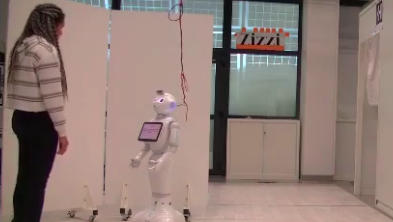
\includegraphics[width=0.49\linewidth]{figures/chapter3/lab1.png}}\hfill
   \subfloat[A person being guided, the emulated shop ``H\&M'' is visible.]{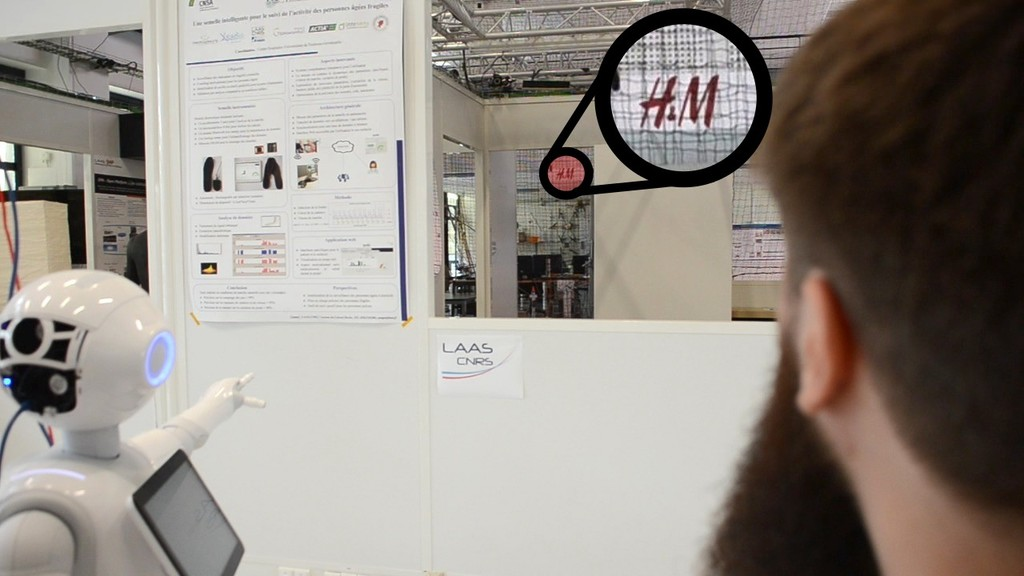
\includegraphics[width=0.49\linewidth]{figures/chapter3/lab4.png}}\hfill
   \subfloat[Two people simulated going to shop. The emulated shop ``Burger King'' is visible in the background and a small part of ``Thai Papaya'' is visible in the foreground.]{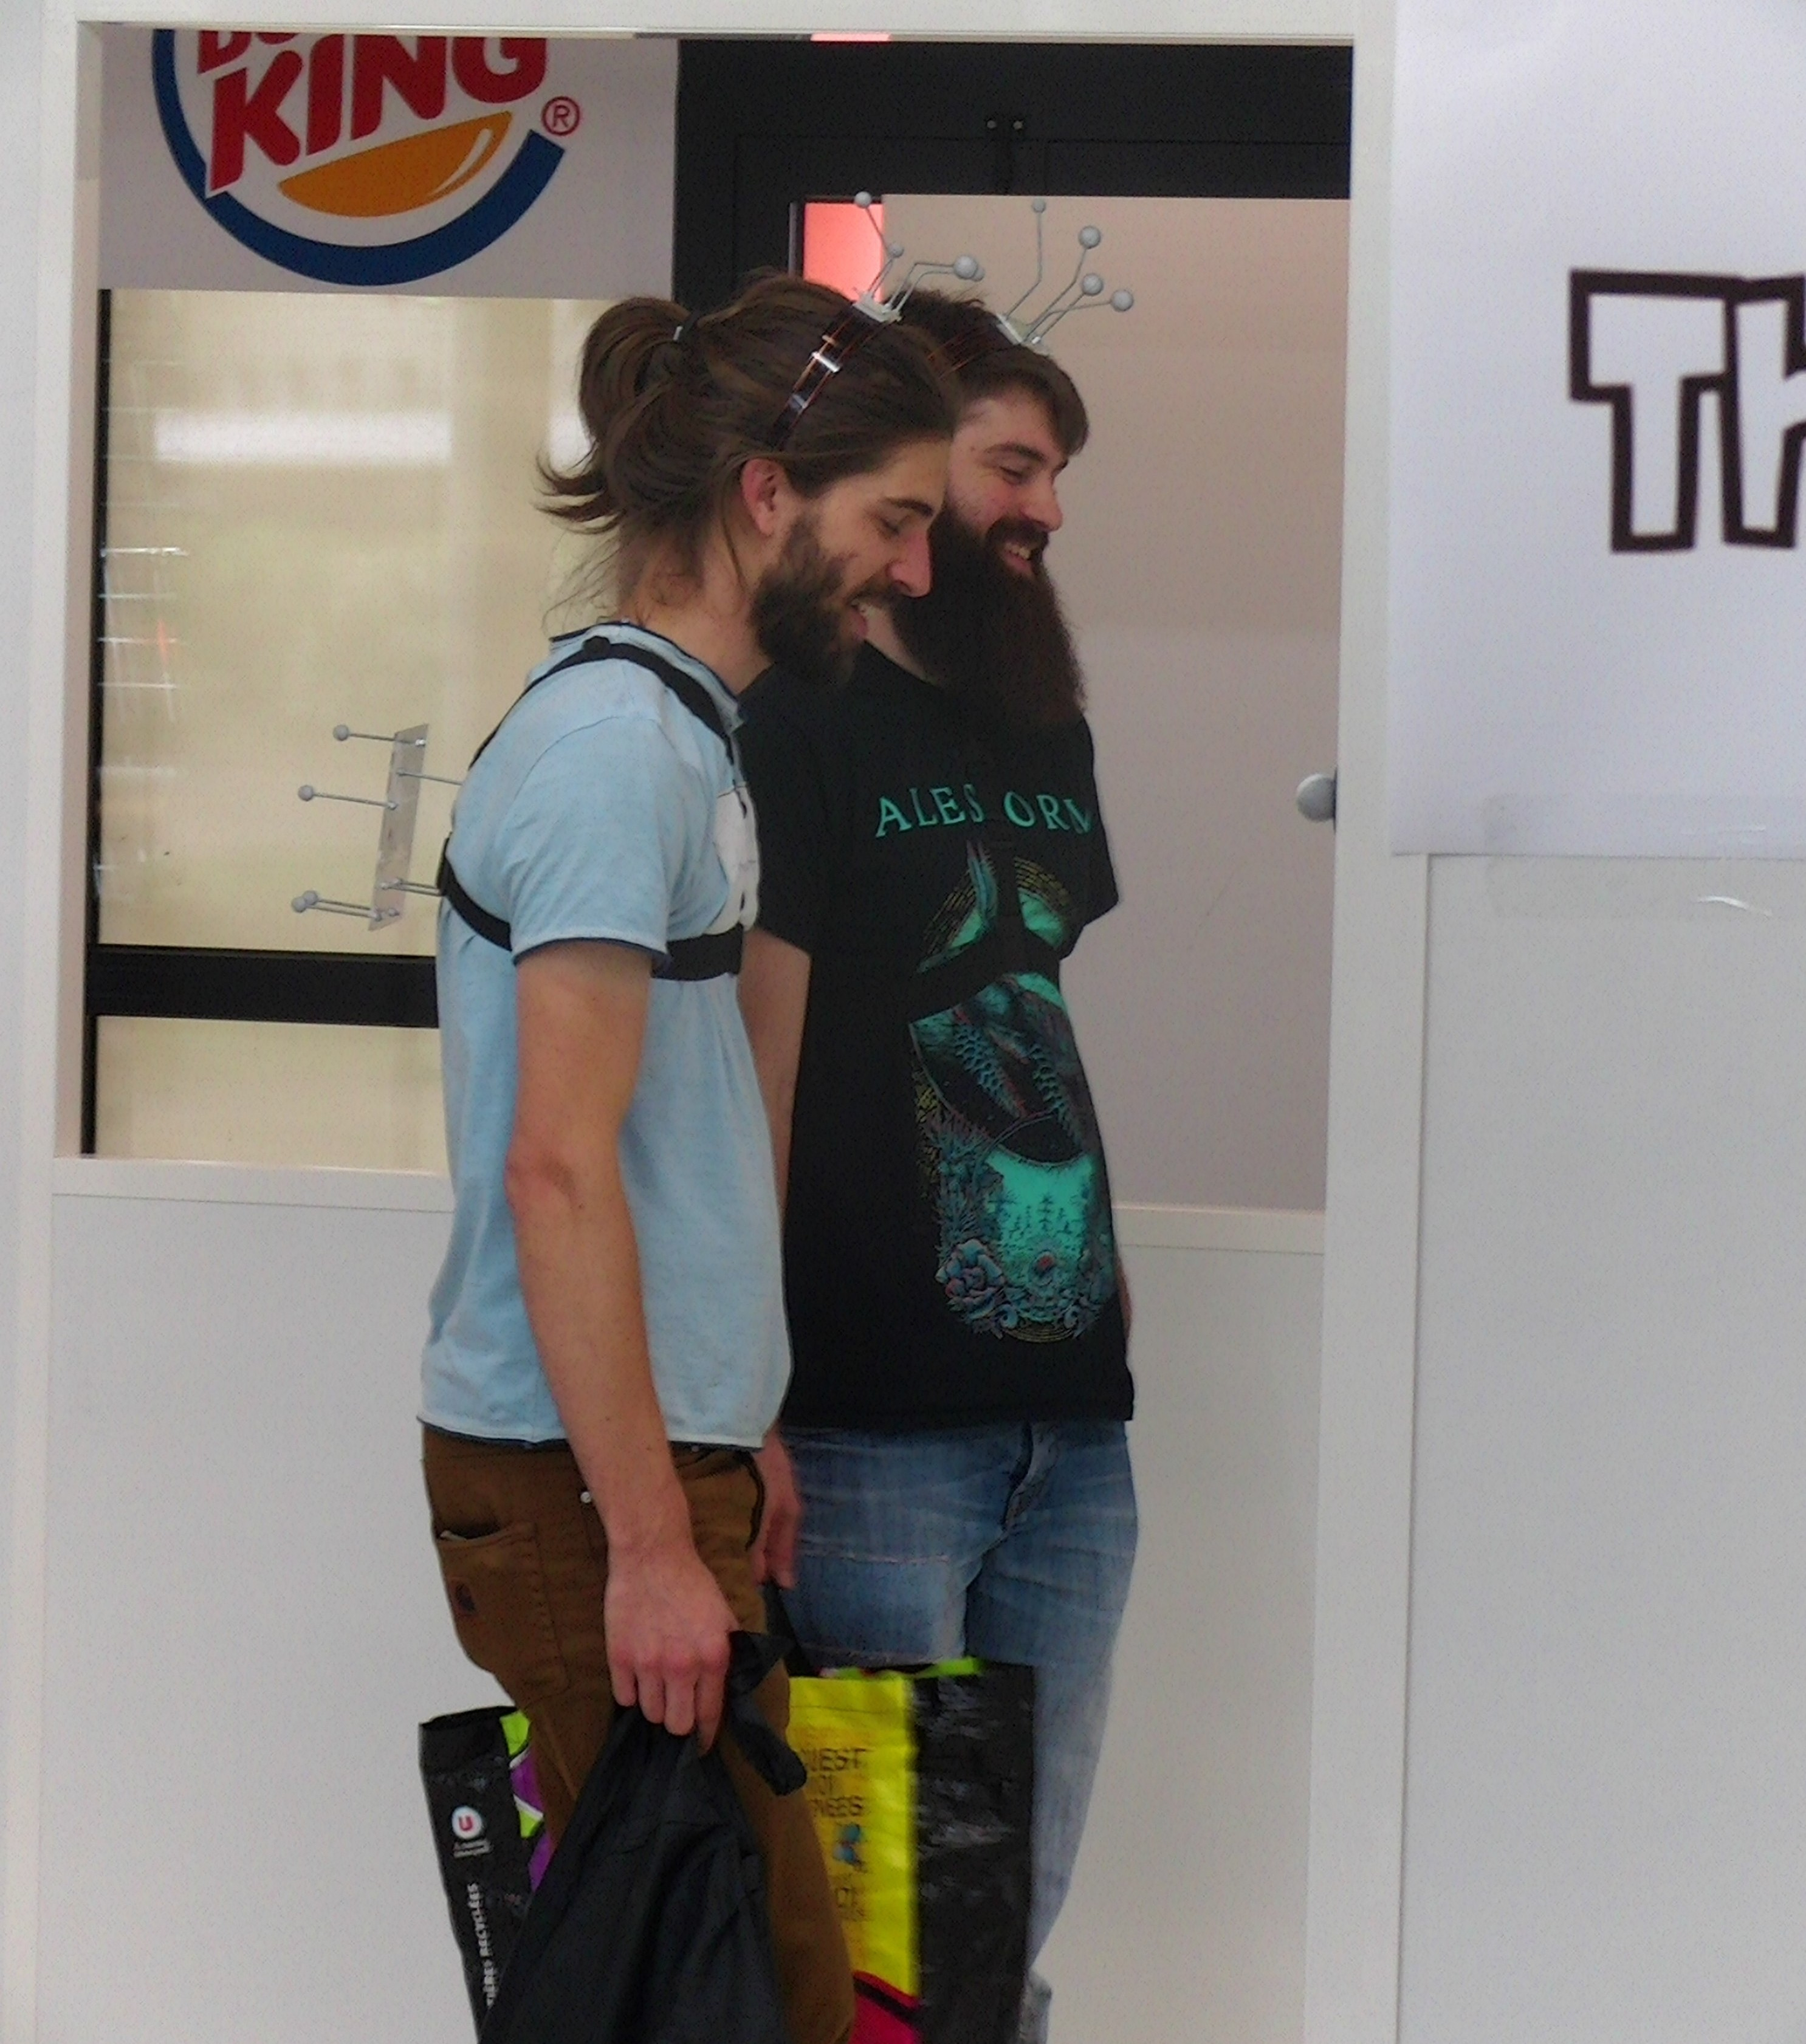
\includegraphics[width=0.49\linewidth]{figures/chapter3/lab3.jpg}}\hfill
   \subfloat[A person being guided, a sign towards the toilet and the shop ``Marco Polo'' are visible on the left of the picture.]{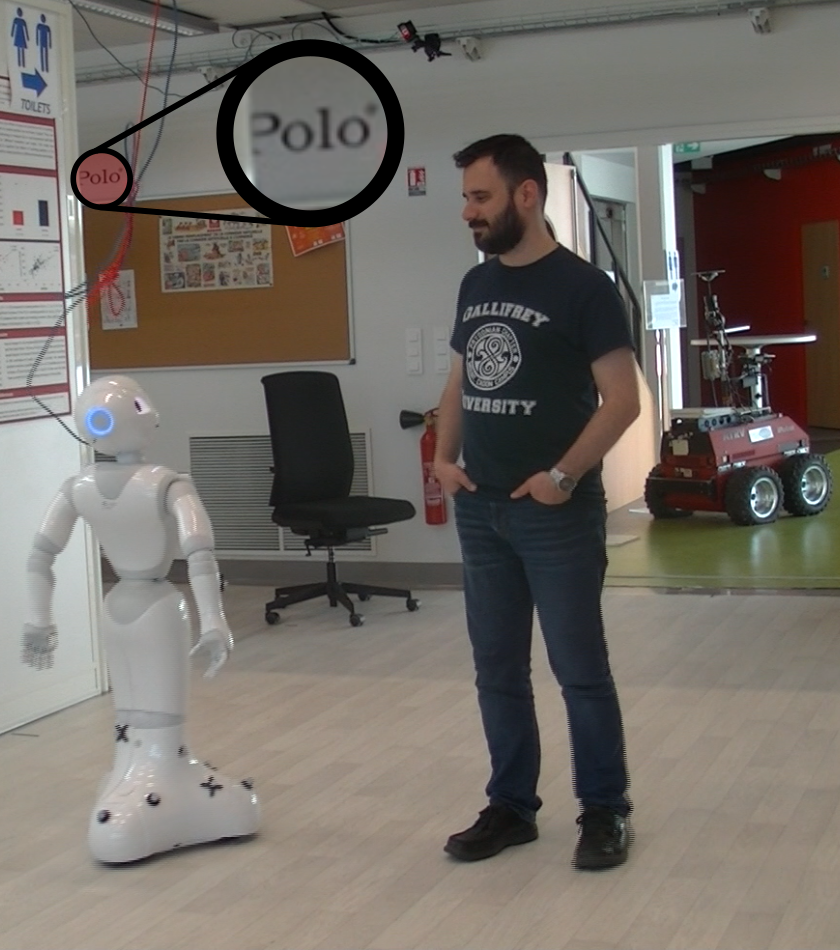
\includegraphics[width=0.49\linewidth]{figures/chapter3/lab2.png}}\hfill
   \caption{Examples of emulated shops of the Finnish mall in our lab.}
   \label{fig:chap3_lab_shops}
\end{figure}

\subsection{Environment and robot setup in the Finnish mall}\label{subsec:setup_mall}
Our architecture has been tested and deployed in a mall in Finland. As we explained previously, it has two abilities: chat with people and guide them, but in this chapter we consider only the latter. The robot was able to interact in English and Finnish, though due to the vast linguistic differences between the two languages, the two versions have been kept separated, and the whole interaction can either be in one or the other. 

\subsubsection{The robot home-base}\label{chap8:subsubsec:home}

For availability for as many customers as possible, the robot was contained in a defined place in the mall as shown in figure~\ref{fig:chap3_pepper_mall}. A home base was designed with the participation of all the project partners. It was a 4 per 4 meters area with a 2.5m high frame structure on it. The home base included a non-reflecting carpet on the floor and an acoustic ceiling surface on the roof.

\begin{figure}[ht!]
	\centering
	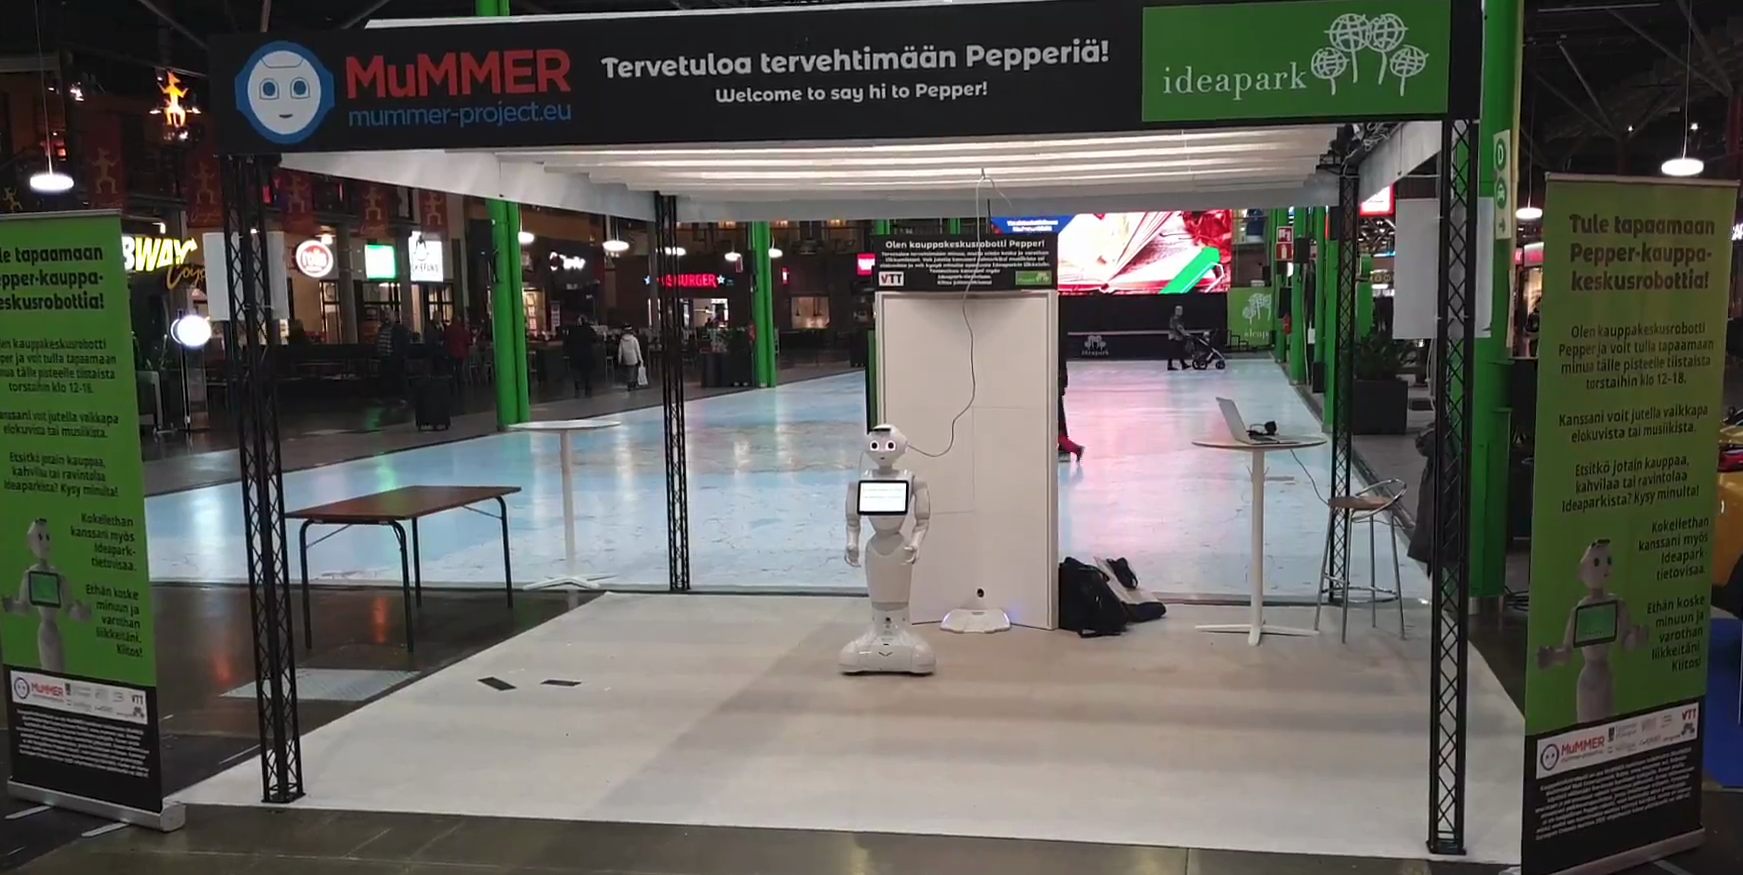
\includegraphics[scale=0.2]{figures/chapter3/pepper_mall.png}
	\caption{\label{fig:chap3_pepper_mall} The pepper robot in its interaction area in the Finalnd mall, Ideapark. }
\end{figure}

During the first deployment in the real mall, we have updated both the Geometric Representation with actual measurements and the \acrfull{ssr} by making sure the regions, interfaces, corridors and intersections were represented reflecting the actual mall topology. To ensure the correctness of the instructions given by the route handler, we generated routes from the deployment location to several shops in the mall and followed them to the destination. Inaccuracies, as well as algorithmic flaws, have been fixed using this method. We also tested the interaction in the Finnish language with our native Finnish partners and corrected some mistakes in the route verbalization.

\subsubsection{Hardware architecture}\label{subsec:hw}
The robot is an upgraded, custom version of the Pepper platform~\cite{caniot_adapted_2020}, which is equipped with an Intel D435 camera and an NVIDIA Jetson TX2 in addition to the traditional sensors that are found on the previous versions of the robot. We used the Robot Operating System (ROS) to enable inter-process communication between the processing nodes. All the streams (audio, video, robot states) are sent to a remote laptop which performs all the computation. The laptop has an NVIDIA RTX 2080 graphics card (for the visual perception system) and 12 CPU cores. The 4 microphone streams are processed at a frequency of $16000$~Hz, and the full perception system delivers the output at 10~fps.

\subsection{Pre-deployment in the Finnish mall, in-situ tests}\label{subsec:tests_mall}

Three integration sessions, each lasting one week, have been made in September 2018, June 2019 and September 2019, in the mall in Finland. The whole LAAS developer team were part of these integration weeks, along with our project partners. So, the author spent around 150 hours (3 times 5 days) in the mall for software integration debugging with the other developers, and testing and debugging of the direction-giving task. 
During the integration weeks, only expert users (developers) interacted with the robot for testing purpose. 

To have a working system in the lab and to have a working system in a real-world site are two different things. As much as a team prepare for an in-situ deployment, there will always be elements that will need to be tuned on site and unexpected bugs arising. Thus, the author had to handle a lot of contingencies, diagnosing where the issue came from, repairing if it was originating from my software, communicating with the person responsible for the component having a bug if it was not from mine, and testing again.

The first step to perform for us once on site was to update both the Geometric Representation (see Sect.~\ref{subsec:models}) which was previously based on architectural plans and refined with actual measurements and the \acrlong{ssr} (see Sect.~\ref{subsec:models}) by making sure the regions, interfaces, corridors and intersections were represented reflecting the actual mall topology. Moreover, it had to be done again to each integration session because shops often changed.

Then, to ensure the correctness of the instructions given by the route handler, we generated routes from the deployment location to random shops in the mall, and followed them to the destination. \acrshort{ssr} inaccuracies as well as algorithmic flaws have been fixed using this method. We also tested the interaction in Finnish language with our native Finnish partners and corrected some mistakes in the route verbalization.


\subsubsection{Component integration problematic}
Even though components were integrated together before getting on site, code modifications and intense testing can make new bugs appear. So, it was essential to test the overall task, \ie the integration between all the components before the final deployment.

Finally, once everything was running quite nicely, some time was dedicated to fine-tune the direction-giving task, ensuring all the components could withstand running for several hours in a row, with naive users possibly interrupting the task at any stage. 

\subsection{``In the wild'' deployment}\label{subsec:deploy}
\begin{figure}
	\centering
	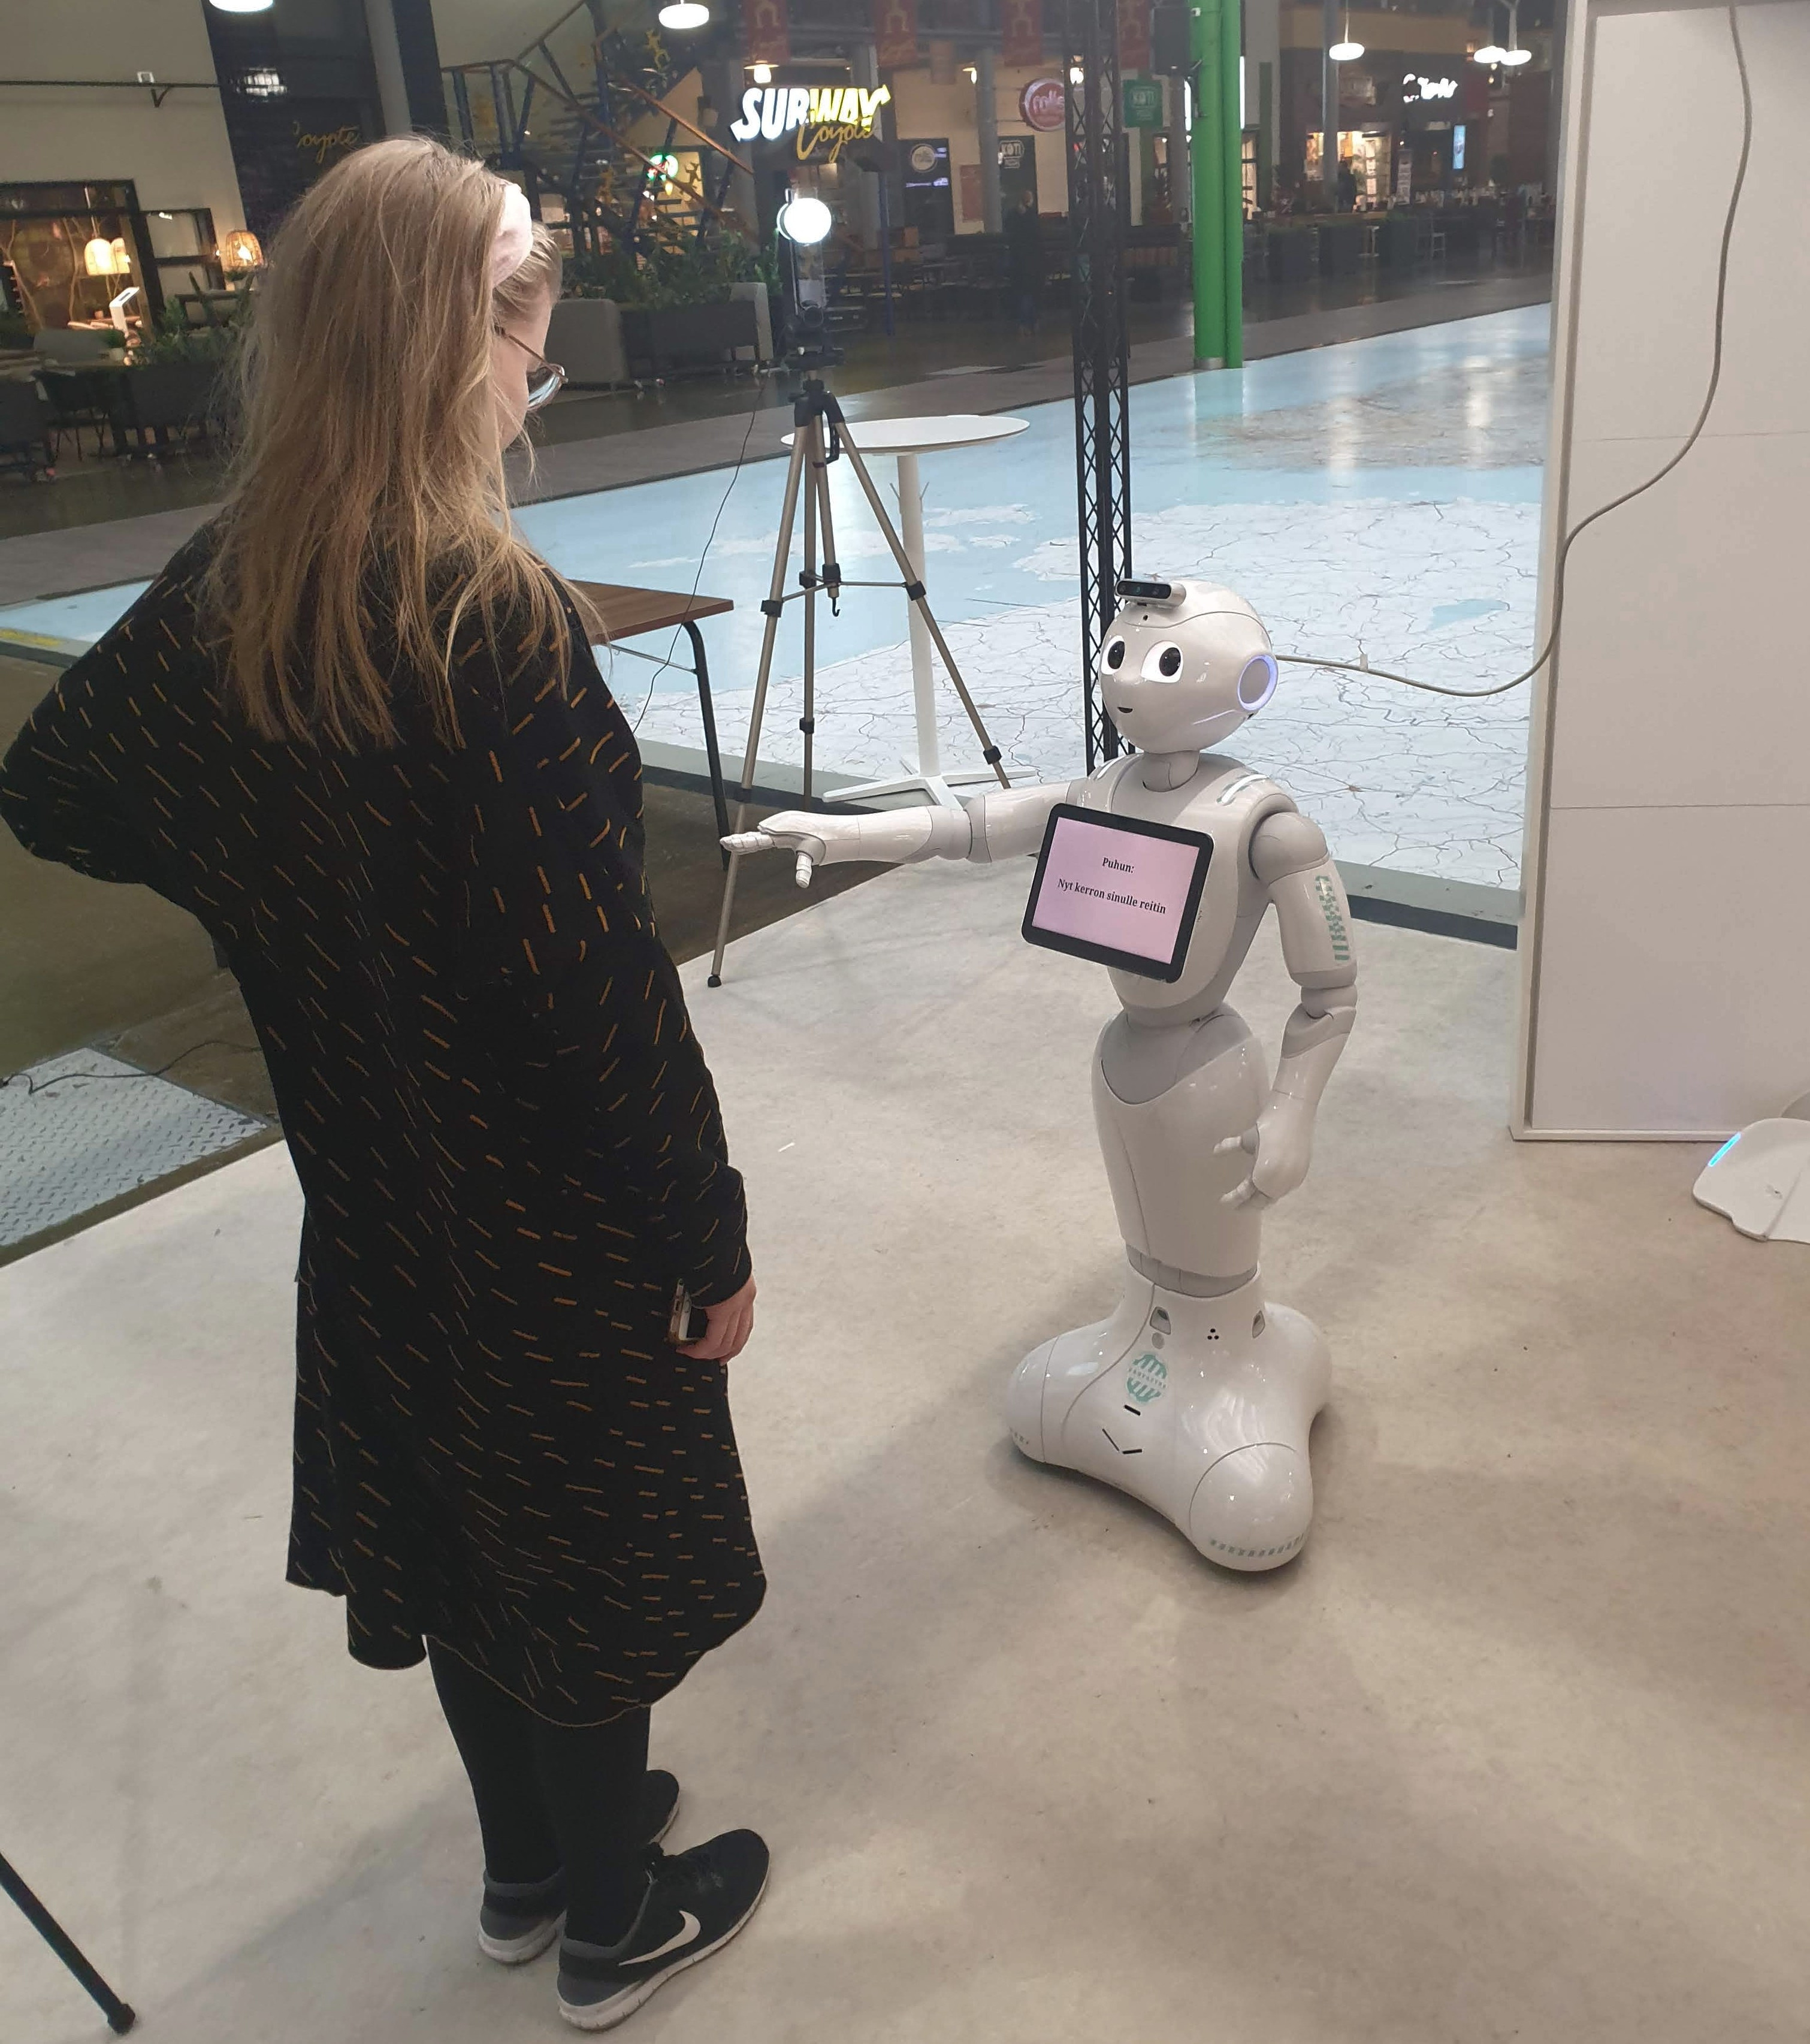
\includegraphics[width=0.5\linewidth]{figures/chapter3/guided_person.jpg}
	\caption{A person receiving directions from Pepper. (Image from VTT team)}
	\label{fig:guided_person}
\end{figure}
The robot was then installed for a long-term 14 weeks deployment from September 2019 to December 2019. During this period, the robot interacted with everyday clients of the mall, who may never had the chance to interact with a robot before. The robot was active for 3 hours per day, three days a week. As it was a project with multiple partners, it was not always possible to have our direction-giving task running. The direction-giving task has been available on the robot 32 days out of the 42. Indeed, the 10 other days, the robot was needed by our project partners to make their own experiments. 

Nowadays, having an autonomous robot in the wild is a challenge. At first glance, we could think that if the robot is able to run smoothly for a few hours, the challenge would be met. However, there are a lot of other elements to take into account. First, how to guarantee the safety of children and elderly? How to ensure that the robot will not fell on or bump into them despite the robot sensors, hurting them? Furthermore, not only people safety is important but making sure that the robot is not damaged by people as well. People might indeed be brutal towards the robot, on purpose or not. 

The project consortium tackled the two safety issues (people safety and robot safety) by hiring a ``robot guard'' and by putting a sign notifying parents to not leave their children alone with the robot. During the robot active hours, this guard employee was physically present to ensure people were respectful towards the robot, \ie not hitting it or pulling it, to watch the kids who may get too close to the robot when it could have moved so they would not risk to be hurt, and to answer people who wanted to know more about the robot or the project than what was explained on the explanatory posters. She was also responsible for starting and shutting down the robot at the beginning and at the end of the half-day. Besides, for security and legal responsibility reasons, we chose to not have the robot navigating during this deployment as it would have been a complicated issue if the robot bumped into someone, especially a kid who could be hurt. It would have been possible if Pepper had a remote emergency stop which could have been given to the guard. Therefore, the step \emph{Ensuring correct placement} was removed in this context. Then, the Human-Aware Navigation component (see Sect.~\ref{subsec:navigation}) was disabled and the Shared Visual Perspective Planner (see Sect.~\ref{subsec:svp}) was only used to compute the 360 degrees visibility of a landmark from the person position.

To tackle the ``obvious'' issue, making sure that the robot continuously running, it was remotely watched by an on-call developer of the project team. At the beginning of the time slot, they launched all the software on the robot. Then, they checked through component monitoring, time to time, if everything was running properly, and they were in contact with the robot guard who told them if she noticed something wrong with the robot. They also had access to a video feed of the robot home-base if needed. Thus, all along this long-term deployment, we adjusted parameters and fixed bugs, with the help of the on-site team VTT and the robot guard that tested the direction-giving task when we asked her. The bugs we encountered concerned mainly Finnish translation issues (\eg ``just after Arnold's'' was translated ``paikan päälle Arnolds'' in Finnish but the correct way to say it in Finnish was ``paikan Arnolds jälkeen'' thus we changed the English sentence into ``right after the place Arnolds'' to be able to get this translation), shop names issues (\eg Finnish people use the utterance ``Hennes Mauritz'' and not ``H\&M'' which was the name in the robot ontology originally) and route issues (\eg a route has one more turn than it should have).

In total, the robot ran the direction-giving task during approximately 96 hours ``in the wild''. Out of these 96 hours, it was interacting with someone during 45 hours. Table~\ref{tab:stats_sessions} summarizes statistical data about the interaction sessions and Table~\ref{tab:stats_tasks} summarizes statistical data about the direction-giving tasks.

\begin{table}[htp]
	\centering
	\begin{tabular}{p{0.8\linewidth}|p{0.1\linewidth}}
		\hline
		Description & Value \\ 
		\hline
		Number of occurred interaction sessions between a human and the robot &  979 \\ 
		Cumulative duration of the interaction sessions  & 2720 min \\ 
		Minimal duration of an interaction session  & 0.1 min \\ 
		Maximal duration of an interaction session & 41 min \\
		Average duration of an interaction session & 2.8 min \\
		Standard deviation of sessions duration & 3.3 min \\
		Average number of direction-giving tasks during a session & 1.1 \\
		Percentage of sessions terminated by goodbyes & 30\% \\
		Percentage of sessions terminated by the participant not perceived by the robot anymore & 70\% \\
		\hline
	\end{tabular}
	\caption{Statistics on interaction sessions in the wild}
	\label{tab:stats_sessions}
\end{table}


\begin{table}[htp]
	\centering
	\begin{tabular}{p{0.8\linewidth}|p{0.1\linewidth}}
		\hline
		Description & Value \\ 
		\hline
		Number of occurred direction-giving tasks between a human and the robot &  1156 \\ 
		Cumulative duration of the direction-giving tasks & 930 min\\ 
		Minimal duration of a direction-giving task & 0.01 min \\ 
		Maximal duration of a direction-giving task & 22 min \\
		Average duration of a direction-giving task & 0.8 min \\
		Standard deviation of direction-giving tasks duration & 1.27 min \\
		Success rate of the step \emph{Establishing the shared goal} & 63\% \\
		Success rate of the step \emph{Route planning according to the human willingness and ability to climb stairs} & 100\% \\
		Success rate of the step \emph{Pointing to target} & 56\% \\
		Success rate of the step \emph{Ensuring target seen} & 39\% \\
		Success rate of the step \emph{Pointing to passage and giving route directions} & 94 \% \\
		Success rate of the step \emph{Ensuring passage seen or route understood} & 92\% \\
		Success rate of the removed step \emph{Check if indications understood} & 19\% \\
		\hline
	\end{tabular}
	\caption{Statistics on the direction-giving task in the wild. \emph{Ensuring target seen} is a part of the step \emph{Pointing to target} as described in Sect.~\ref{sec:guiding}. Likewise,  \emph{Ensuring passage seen or route understood} is a part of the step \emph{Pointing to passage and giving route directions}. The success rate of a step is the number of times the given step has been achieved over the number of times it was planned (\eg \emph{Route directions and pointing} is not planned if there is no passage to point), all direction-giving tasks combined. Steps were not achieved sometimes because of robot failures but most of the time it was because the human was leaving during the task. As mentioned in Section~\ref{par:route_understood}, we did not keep the step \emph{Check if indications understood} all along the deployment because, as shown by the success rate, people were leaving before answering this question. Then, as this step was considered as superfluous by users, we merged it with the one before, \emph{Ensuring passage seen}.}
	\label{tab:stats_tasks}
\end{table}

\section{User Study}\label{chap8:sec:us}

As presented in the introduction (Section~\ref{chap8:sec:intro}), we performed a study with the mall customers in January 2020, on one week, after the 14 months deployments. It was carried out in collaboration with Kathleen Belhassein, the leader of this study. She elaborated the study procedure and performed the analysis of the collected data. And, she participated in the organization and implementation of the study, the creation of the behavioral video coding scheme, and the video coding. The author was in charge of the robot, and participated in the organization and implementation of the study, the creation of the behavioral video coding scheme, and the video coding. 

For us roboticists, this study was a user study aiming at evaluating our robotic architecture and our task design. Aside, for Kathleen Belhassein, a psychologist, this study was an experimental study aiming at evaluating the impact of the communicative strategies used on the effectiveness and quality of the interaction.

Thus, we compared three different versions of the direction-giving task performed by the robot and their impact on the quality of interaction perceived by the customers: is the route description more efficient if the robot positions itself in space to point, taking the perspective of its interlocutor? Is the interaction more pleasant for the users? Is the quality of the interaction perceived as better? 

We had also intended to compare the quality of interaction perceived by the customers with the \acrshort{qoi} computed by the robot (see Chapter~\ref{chapter:chap7}) but the \acrshort{qoi} Evaluator was not refined enough at the time of the user study to make that happen.

More precisely, we had chosen to compare three versions of the system, each time with the robot fully autonomous:
\begin{bulletList}
	\item Condition 3 : Dialogue + Pointing + Navigation \\
	\ie the complete system -- as described in Section~\ref{sec:globalarchi}
	\item Condition 2 : Dialogue + Pointing \\
	\ie the system used during the 14-weeks deployment (see Section~\ref{subsec:deploy}) -- the subtask ``Ensuring Correct Placement'' was removed (see Figure~\ref{fig:chap3_SM})
	\item Condition 1 : Dialogue only \\
	\ie the system used during the 14-weeks deployment less the pointing --  the subtask ``Ensuring Correct Placement'' was removed as well as the pointing actions
\end{bulletList}

In Condition 1, the robot performed the task only through dialogue. It verbally explained the route to be taken without ever pointing to an element or moving. Condition 2 integrated pointing gestures in parallel with the dialogue, with the possibility to rotate on itself to be able to point to the desired element (\eg if the target was behind it). Finally, Condition 3 was performed with the complete system as presented in Section~\ref{sec:globalarchi}, reasoning on the participant's perspective to move so that the participant can see the pointed element.

In the user study context, the possible content of the dialogue task was identical for all participants (except in the case of the last item): 

\begin{bulletList}
	\item Introduction: ``Hi, my name is Pepper, I can help you find your way...''
	\item Target: Verbalization of the direction of the desired store
	\item Route: Verbalization of the route directions to take to get to the desired store
	\item Comprehension question: ``Did you understand?'', ``Have you seen the intersection?''
	\item Repetition: ``Should I show you again?''
	\item Repositioning face: ``Please, come in front of me''
	\item Repositioning distance: ``Can you come closer?''
	\item Lateral repositioning: ``Can you make a few steps on your left/right, please?''
	\item Announcement of a move: ``I'm going to move so I can show you.''
	\item Announcement of path explanation: ``Now I'm going to explain to you the route.''
	\item OK
	\item End of interaction: I'm happy that I was able to help you. Okay, let's talk about something else...''
	\item Other: The chatbot starts up and the robot says something unrelated to the task at hand, it happens when the speech recognition does not understand what the human said
\end{bulletList}

Some items, such as repositioning requests or move announcements, were not present in the Conditions 1 and 2.

\bigskip

Our objective was to confirmed that the Condition 3, our complete system, was preferred over the Conditions 1 and 2 as it implemented a shared perspective between the robot guide and the human (see Section~\ref{subsec:svp}).

\subsection{Experimenters}

Two experimenters were present and visible to the participants in order to manage the registration systems and the visitors of the mall, to ensure the smooth running of each participation, and to administer the questionnaires as well as the effectiveness test. A third experimenter (the author), being hidden from the participants by a panel, managed the software. Some parameters of the Supervisor had to be manually changed to switch between conditions. Thus, the Supervisor was launched at the beginning of a condition and killed at the end. The other software were usually launched at the beginning of the day and ran until night, except if bugs were encountered. This launch of the Supervisor was the only moment in a condition during which the experimenter intervened, otherwise the robot was acting completely autonomously. A fourth experimenter, from VTT, was present to provide translation and conduct the experiment in Finnish.

\subsection{Participants}

In total, 34 participants took part in this study. There were 22 women and 12 men, and their ages ranged from 20 to 68 ($M=37.12$, $SD=10.22$). All were shoppers at the Ideapark shopping center. Participants were recruited through a website\footnote{\url{https://sites.google.com/view/pepper-exam/home}} combined with a recruitment questionnaire\footnote{\url{https://forms.gle/bNMfSFVHznAPw9BS9}}, published in the mall the previous weeks. All participants completed a consent form and an image rights release form (see Appendix~\ref{app:consent_form} for the English version and Appendix~\ref{app:consent_form_fi} for the Finnish version given to the participants). The experiment lasted approximately 40 minutes for one participant, and was located in the robot interaction area (see Figure~\ref{fig:chap3_pepper_mall} and Section~\ref{chap8:subsubsec:home}).

9 participants were excluded from the analyses due to technical problems during the experiment, which could later interfere with their evaluations of the different systems. Most often, it was the chatbot which would start as the Dialog had not understood properly what had said a participant and so started to talk about a completely different subject. Thus, 25 participants were included in the analysis, 17 women and 8 men with their ages still ranging from 20 to 68 ($M=37.12$, $SD=10.11$).

\subsection{Tools for Data Collection}

In order to collect the participants' opinions about each condition, we prepared two questionnaires for them to fill: \acrshort{perdita}, a questionnaire dedicated for \acrshort{hri} user studies and a questionnaire that we devised for this particular user study. These questionnaires were presented in Finnish to the participants (both of them were translated double-blind). At the end of each condition, each participant had to fill both.

Moreover, all interactions were recorded which allowed us to analyze the videos, noticing participants' gazes and moves.

\subsubsection{\acrshort{perdita} Questionnaire}

The robot decisions were evaluated by the participants with the questionnaire \acrfull{perdita}~\cite{devin_2018_evaluating}. It was developed at LAAS-CNRS and has been proposed to the robotic community as a basis for the development of a tool to evaluate the decisional aspects of a robotic agent in a joint action. It is not specific to a robotic platform or to a particular task. It has several dimensions, as presented in Table~\ref{chap8:table:perdita}, and each of them measure a specific aspect of joint action. The questionnaires are visible in Appendix~\ref{app:perdita} for the English version of the questionnaire and Appendix~\ref{app:perdita_fi} for the Finnish version of the questionnaire which was given to the participants.

\begin{table}[]
	\centering
	\resizebox{\textwidth}{!}{%
		\begin{tabular}{c|c|c}
			Dimension & Question & Item \\\hline\hline
			Collaboration &
			\makecell{In your opinion, \\ the collaboration with the robot was:} &
			\begin{tabular}[c]{@{}c@{}}Restrictive/Adaptive\\ Useless/Useful\\ Not satisfying/Satisfying\\ Confusing/Acceptable\\ Not effective/Effective\end{tabular} \\ \hline
			Interaction &
			\makecell{In your opinion, \\the interaction with the robot was:} &
			\begin{tabular}[c]{@{}c@{}}Negative/Positive\\ Not convenient/Convenient\\ Complicated/Simple\\ Ambiguous/Clear\\ Unpleasant/Pleasant\end{tabular} \\\hline
			Perceived robot skill &
			\makecell{In your opinion, \\the robot is rather:} &
			\begin{tabular}[c]{@{}c@{}}Unresponsive/Responsive\\ Not efficient/Efficient\\ Unintelligent/Intelligent\\ Incompetent/Competent\end{tabular} \\\hline
			Verbal &
			\makecell{In your opinion,\\ the robot speech was:} &
			\begin{tabular}[c]{@{}c@{}}Useless/Useful\\ Inappropriate/Appropriate\\ Unpredictable/Predictable\end{tabular} \\\hline
			Action &
			\makecell{In your opinion, \\ the robot chose to act in a way which was:} &
			\begin{tabular}[c]{@{}c@{}}Appropriate/Inappropriate\\ Inflexible/Compliant\\ Not expectable/Expectable\\Unsafe/Reassuring\end{tabular}
		\end{tabular}%
	}
	\caption{English translation of the questions for each dimension of \acrshort{perdita} (see~\ref{app:perdita}). The used questionnaire, in Swedish, is in Appendix~\ref{app:perdita_fi}.}
	\label{chap8:table:perdita}
\end{table}

\subsubsection{Additional Questionnaire}
An additional questionnaire was used to collect the participants' evaluation of the overall quality of the interaction (see Appendix~\ref{app:add_questionnaire} for the English version and Appendix~\ref{app:add_questionnaire_fi} for the Finnish version given to the participants). Originally, we devised this questionnaire in order to comparer its result with the \acrshort{qoi} measured by the robot (see Chapter~\ref{chapter:chap7}). However, as the integration of the \acrshort{qoi} Evaluator was not mature enough at the time of the user study, we did not have data computed by the robot to compare the questionnaire to. But, interestingly, as we will see in Section~\ref{chap8:subsec:us_results}, this questionnaire gave valuable results.

The questionnaire has three items. First, the participants were asked to rate their interaction with Pepper on a scale of -1 (poor) to +1 (good). Two additional open-ended questions were asked: ``Have you seen everything Pepper has indicated to you?'' and ``Did you understand the path you have to take?''. 


\subsubsection{Video Observation}

The interactions between the participants and the robot were filmed by three cameras placed around the interaction area. Fences prevented other mall shoppers from entering the experimental area, and signs indicated the presence of cameras.

The videos were annotated using the software ELAN\footnote{\url{https://archive.mpi.nl/tla/elan}}~\cite{wittenburg_2006_elan}, visible in Figure~\ref{chap8:fig:elan}, in order to analyze communicative elements between the participant and the robot (such as gazes or positions) in terms of frequency of occurrence, durations, and sequences of occurrence. A behavioral video coding scheme was devised prior to the user study, based on the tests conducted in the laboratory, allowing the analysis of these elements. This coding scheme can be found in Appendix~\ref{app:coding_r} for the observed robot behaviors and in Appendix~\ref{app:coding_h} for the observed human behaviors. 

In order to assess the reliability of the behavioral sampling, 50\% of the videos were coded by an observer blind to the hypotheses of the study (\ie the author, who did not know the hypotheses formulated by Kathleen Belhassein at the time of the coding). Consistency between observers measured by the Cohen’s kappa coefficients was higher than 0.8.

\begin{figure}[ht!b]
	\centering
	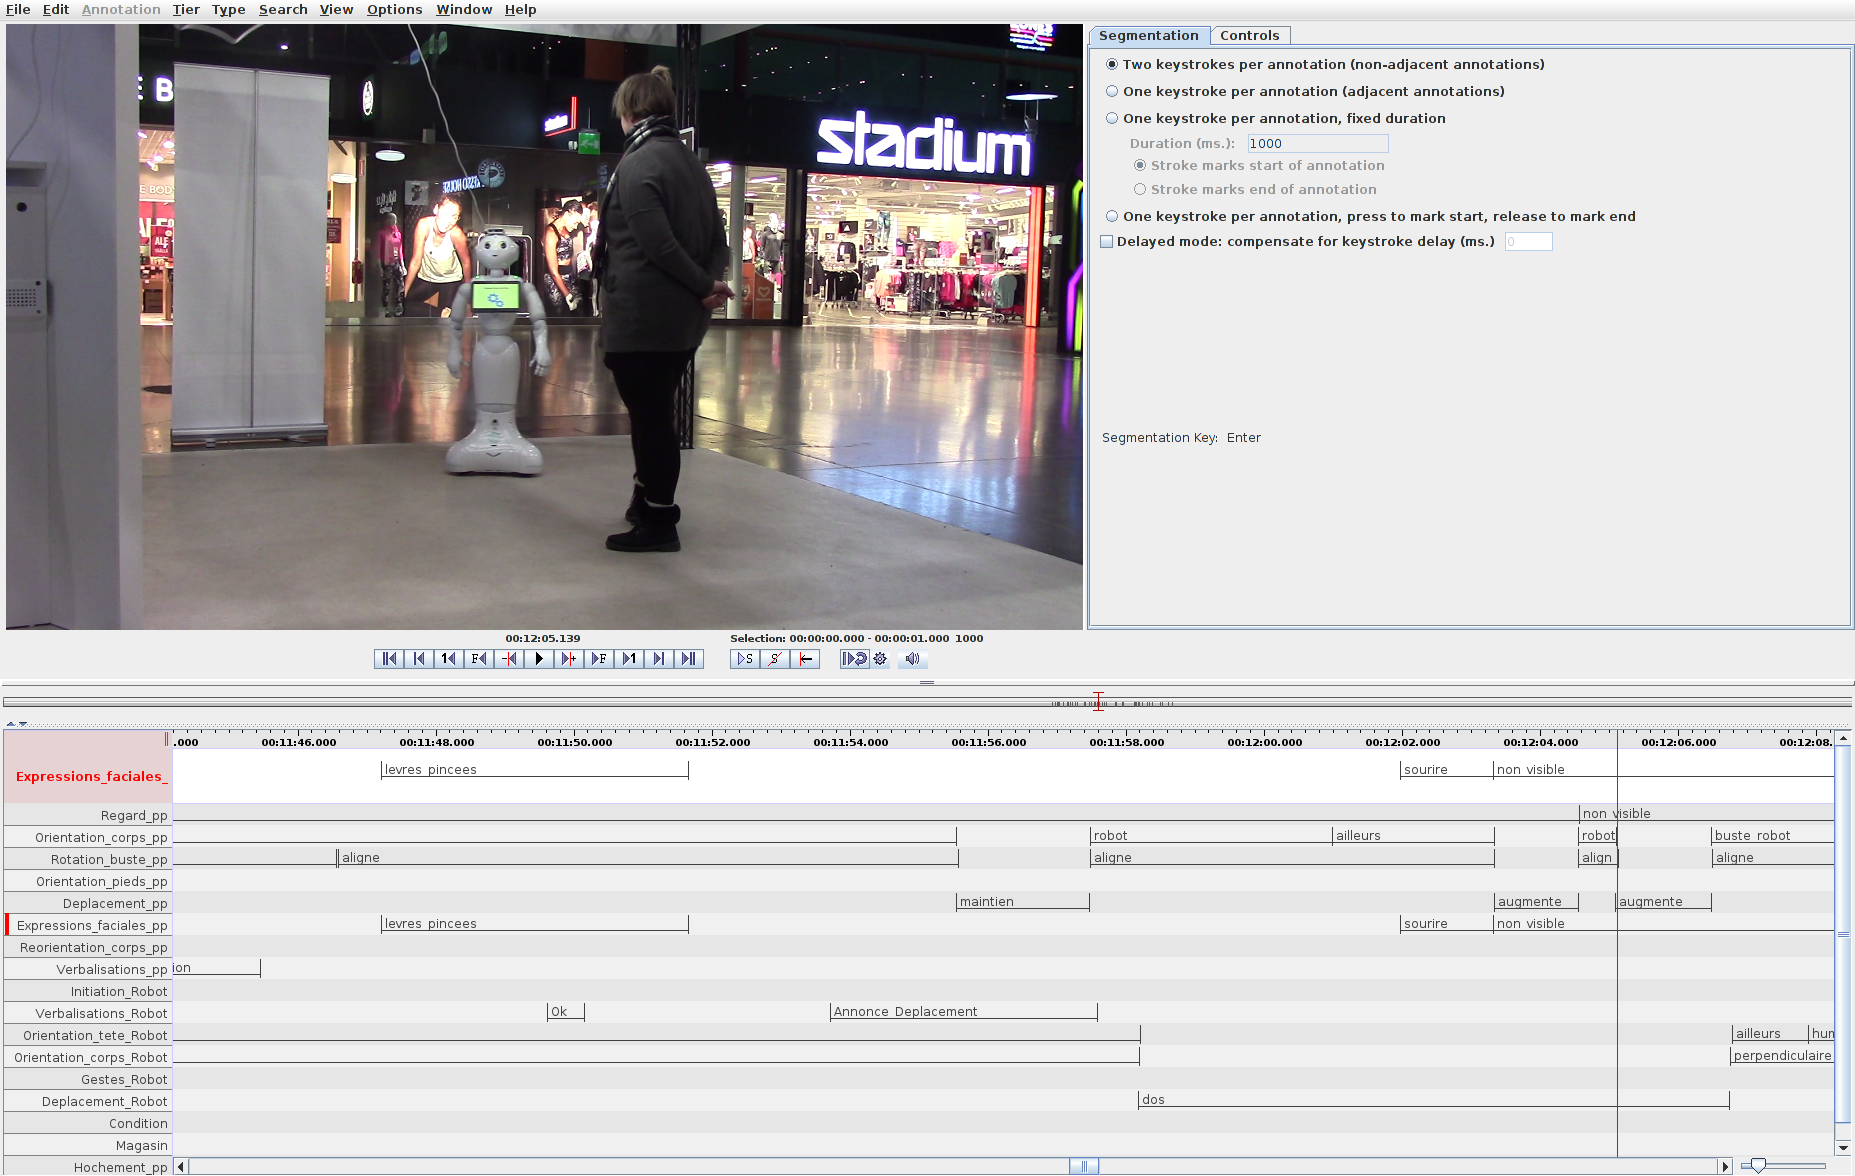
\includegraphics[width=\linewidth]{figures/chapter3/elan.png}
	\caption{Screenshot of the Elan software with the Condition 3 being annotated. Pepper is moving in order to reach the place where it will point at Pentik.}
	\label{chap8:fig:elan}
\end{figure}

\subsubsection{Interview}

After having participated in the three conditions, participants were briefly interviewed by an experimenter from VTT (as they spoke Finnish) to gather their impressions of the three experimental phases. The experimenter first asked the participant if they had noticed anything about the study, especially if they had noticed a difference between the three phases. The experimenter then asked the participant which phase they liked best and why, and which one they liked least. Finally, the participant was told the purpose of the study.


\subsection{Procedure}
The study was a within-subjects experiment, whose goal was to evaluate the impact of three different versions of the system on the effectiveness of the route description and the interaction quality. 

For the participants, the task was to ask the robot where a particular store was located, so that the robot would give them the directions to get there.

The independent variable was the version of the system used. The first version, corresponding to Condition 1, was performed using only dialog (verbal -- Pepper verbally explained the route --, and visual -- content of its speech was simultaneously displayed on the display on its chest). The second version of the system, corresponding to the Condition 2, added the pointing of the passage and the target (eventually rotating to be able to do so). Finally, the last version, corresponding to Condition 3, was performed with the complete system. 

Each participant was confronted with the three conditions, the order being different for each of them.

Three stores of the mall were chosen to be the targets the participants will ask the robot to being guided to. The choice was made based on their visibility and distance from where the robot was deployed: 
\begin{bulletList}
	\item Finnlandia: a store close and visible 
	\item Pentik: a close but not visible store
	\item City Kulta: a distant and not visible store
\end{bulletList}

Stores were also counterbalanced within the conditions.

\subsubsection*{Proceedings of the experiment for one participant}

The participant was first greeted by the experimenters in the interaction area at the time of the appointment. It would sign the consent form and image rights release. The VTT experimenter would then explain to the participant how the interaction would take place, without mentioning the purpose of the study. Next, the participant was asked to come in front of the robot to start a habituation phase\footnote{It was a script written in the Supervisor, using the resource manager to point, the SVP Planner to find a position with a simulated human and the navigation to move. The robot was not aware of the participant during this scripted task.}, in which the robot demonstrated its capabilities and the behaviors it might exhibit during the study. During this phase, the robot would give a route direction, pointing and moving around the participant. 

Before each condition execution, an experimenter would inform the participant for which store they should asked the robot the route. 

The experiment started with one of the condition. The participant would interact with the robot and then, once the direction-giving task was completed, they would go to a desk near the interaction area to fill the questionnaires. Then, it was the same again for the two other conditions. Finally, once the participant had gone through each condition, the interview was conducted.

The participant was then thanked with a 20 euros gift card to be used in one of the Ideapark shops.

\subsection{Results}\label{chap8:subsec:us_results}

In this section, we will present the results obtained from the data analysis for the two questionnaires and the video observation. They were produced by Kathleen Belhassein.

\subsubsection{\acrshort{perdita}}

Data from \acrshort{perdita} were analyzed using the Friedman test, a non-parametric test as the scale (from 1 to 7) does not allow to consider that the gaps of the scale are identical. It is separately performed on each dimension of the questionnaire. To use such a test allows to know if the answers filled by participants for a given dimension and a given condition are significantly different from the ones given for the same dimension in the other conditions. Analyses revealed no significant effect of the conditions in all the dimensions, although Collaboration showed a significant trend, $F(2,25) = 5.96, p = 0.0509$, with the effect size measured by Kendall's W being small ($W=0.1192$). For the other dimensions, the values were: Perceived robot skill ($F(2,25)=5.45, p=0.0655$), Interaction ($F(2,25)=4.89, p=0.0867$), Verbal ($F(2,25)=2.85, p=0.240$) and Action ($F(2,25)=4.98, p=0.0830$).

\subsubsection{Additional Questionnaire}
The interaction score given by the participants when asked to rate their interaction on a scale of -1 to +1 correlated with the Interaction dimension of the PeRDITA questionnaire ($r = 0.85, p<0.05$). The scores were scaled from 0 to 2 (instead of -1 to +1) to ease the analysis. They were analyzed with the Friedman test, since the data do not follow a normal distribution (the Shapiro-Wilk test was significant ($W=0.829, p=7.153e^{-08}$)).

Analysis revealed a significant effect of the conditions on the interaction score of the additional questionnaire ($F(2,25) = 10.7, p<0.01$) with a small effect size ($W=0.215$). Since results were significant, pairwise comparisons were performed with the Wilcoxon test and adjusted p-values using the Bonferroni-Holm method). It shows a significant difference between Condition 1 ($M=1.18, SD=0.69$) and 2 $(M=1.5, SD=0.6; p<0.05$), and between Condition 1 ($M=1.18, SD=0.69$) and 3 ($M=1.56, SD=0.46; p<0.01$) (see Table~\ref{chap8:table:wilcox_QA}). No significant difference was found between Condition 2 and Condition 3 ($p=0.506$).

\begin{table}[!htb]
	\centering
	\resizebox{0.7\textwidth}{!}{%
		\begin{tabular}{ccccc}
			\hline
			 y     & group 1 &  group 2 & adjusted p-value & significant \\ \hline\hline
		Interaction note     & 1     & 2  & \textbf{0.023}       & +   \\ \hline
			Interaction note     & 1     & 3  & \textbf{0.007}       & ++  \\ \hline
		Interaction note & 2     & 3     & 0.506& no  \\ \hline
		\end{tabular}%
	}
	\caption{Results of Wilcoxon signed-rank test on responses about interaction of the additional questionnaire. Comparisons between group 1 and 2 ($p<0.05$) and between group 1 and 3 ($p<0.01$) were significant.}
	\label{chap8:table:wilcox_QA}
\end{table}

Responses to the two open-ended questions in the supplemental questionnaire (``Did you see all the items Pepper showed you?'' (question 1) and ``Did you understand the path you need to take?'' (question 2) were classified into two categories: ``Yes'' and ``No''. The responses indicating that they only partially understood the path, or that they only saw some of the elements shown by Pepper were counted as a negative response. These data were analyzed with Cochran's Q test, a non-parametric test as the data are qualitative with three conditions to compare. Affirmative responses appear to be more frequent in experimental Conditions 2 and 3 (see Figure~\ref{chap8:fig:answer_QA}), which is confirmed by the analyses related to question 1 which show that the answer given depends on the experimental condition ($Q(2,25)=9.1, p<0.05$). 

\begin{figure}[!htb]
	\centering
	
	\subfloat[Stack column chart for the first question]{\label{chap8:fig:answer_q1_QA}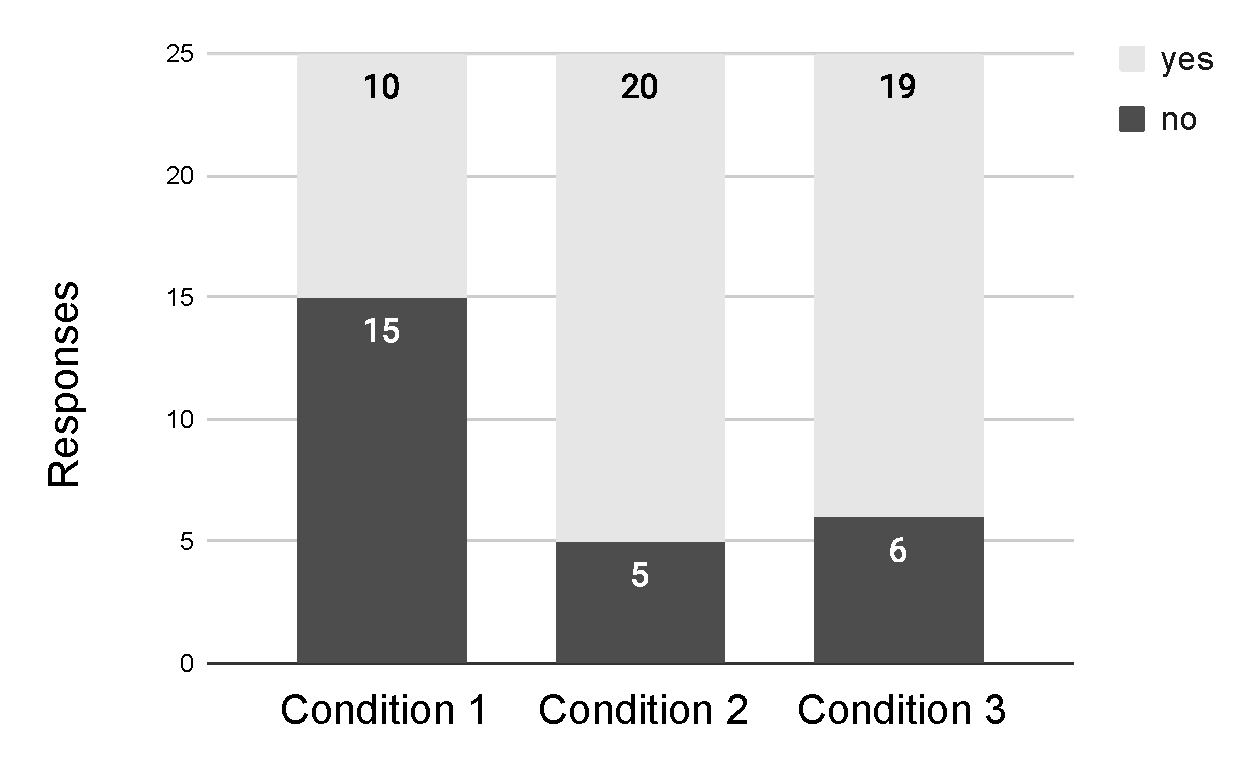
\includegraphics[width=0.49\linewidth]{figures/chapter3/resp_QA_Q1.pdf}}\hfill
	\subfloat[Stack column chart for the second question]{\label{chap8:fig:answer_q2_QA}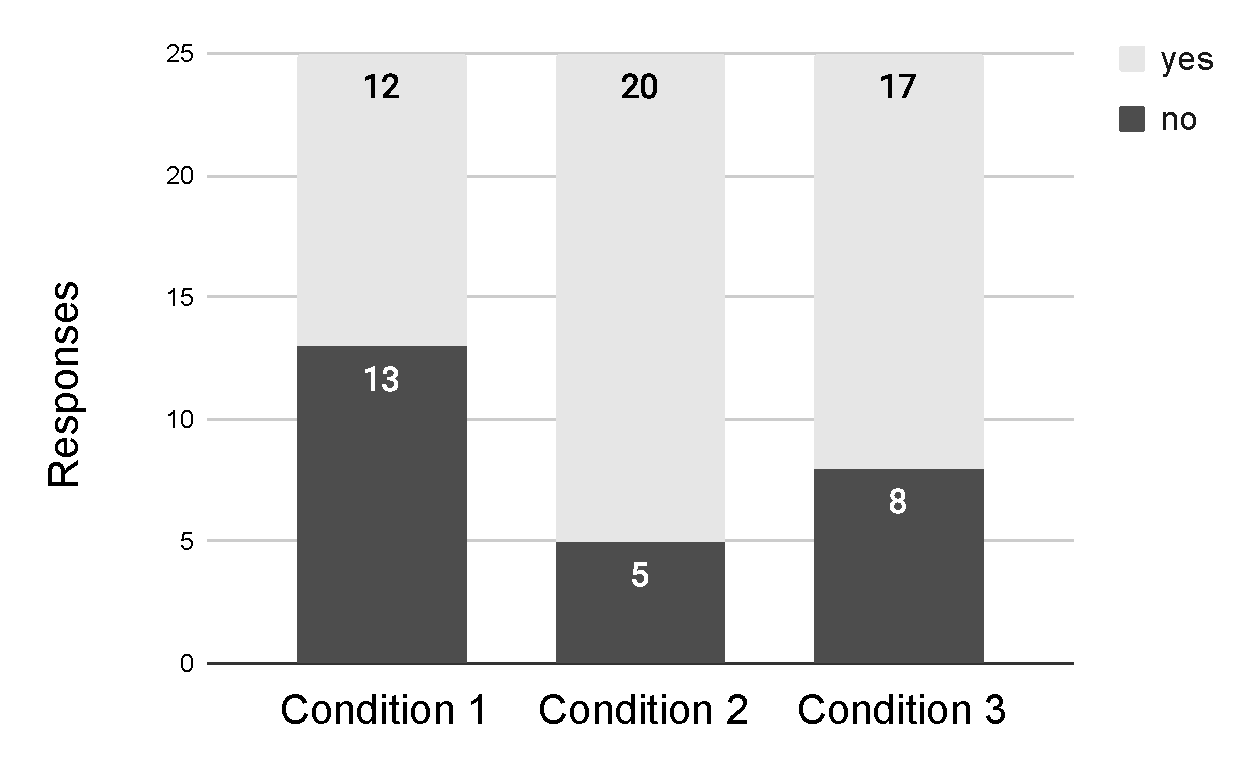
\includegraphics[width=0.49\linewidth]{figures/chapter3/resp_QA_Q2.pdf}}
	\caption{Stack column charts representing the participants answers to the two questions of the additional questionnaire, classified into ``Yes'' and ``No'', according to the condition.}
	\label{chap8:fig:answer_QA}
\end{figure} 


Post-hoc comparisons were performed with the McNemar's test. The difference is significant between Condition 1 and 2 ($p=0.0244$) and Condition 1 and 3 ($p=0.0389$) but not between Conditions 2 and 3. Participants seem to see the items pointed out by Pepper better in Condition 2 and 3 compared to Condition 1. On the other hand, the analysis shows that the type of response given does not depend on the experimental condition for question 2 ($Q(2,25)=5.76, p=0.0560$).

We wanted to investigate the effect of the requested store on the type of answers, independently of the condition (see Figure~\ref{chap8:fig:stores_comp_QA}). For question 1, the type of the given answer does not depend on the store requested, ($Q(2,25)=4.9, p=0.0863$). On the other hand, it does depend on the requested store for question 2, ($Q(2,25)=11.4, p<0.01$). According to McNemar's test, the difference is significant between the stores City Kulta and Pentik ($p<0.05$) but not between the other stores. Participants seem to have more difficulty understanding the path to City Kulta (store far away and not visible) compared to the Pentik store.

\begin{figure}[!htb]
	\centering
	
	\subfloat[Stack column chart for the first question]{\label{chap8:fig:stores_comp_QA_Q1}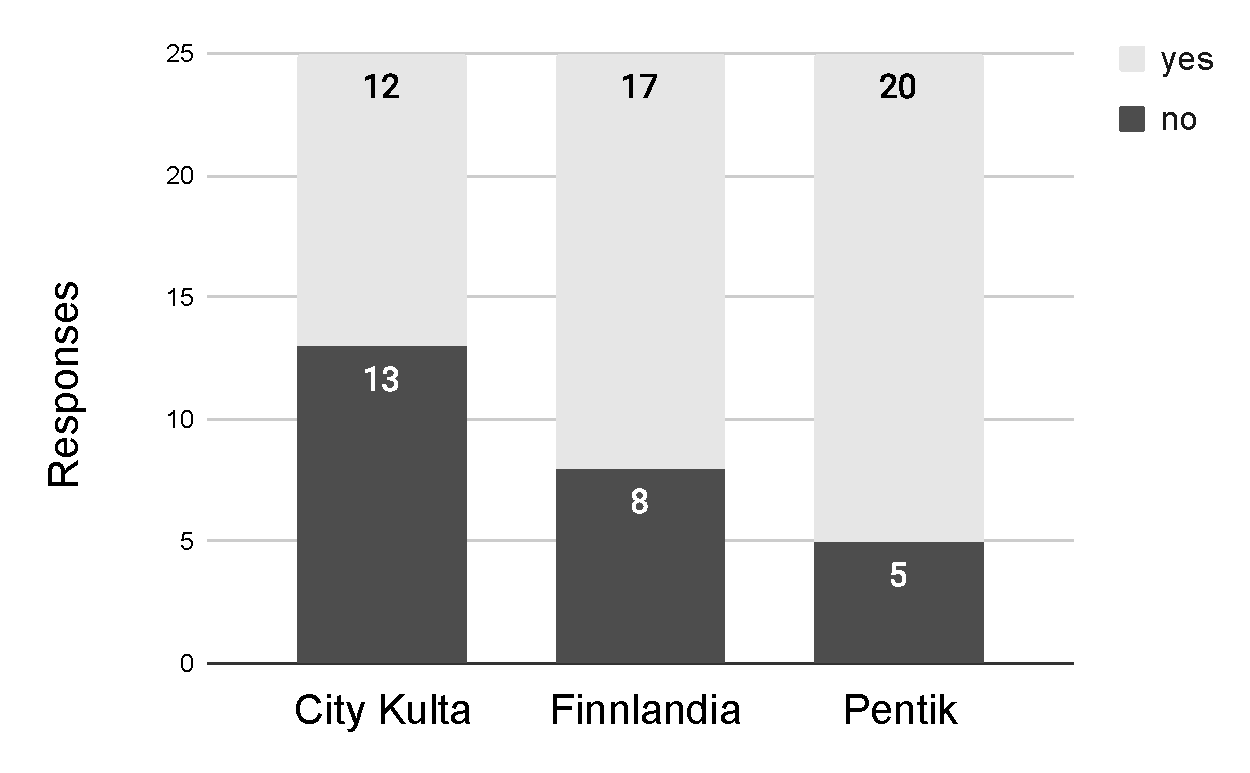
\includegraphics[width=0.49\linewidth]{figures/chapter3/resp_stores_Q1.pdf}}\hfill
	\subfloat[Stack column chart for the second question]{\label{chap8:fig:stores_comp_QA_Q2}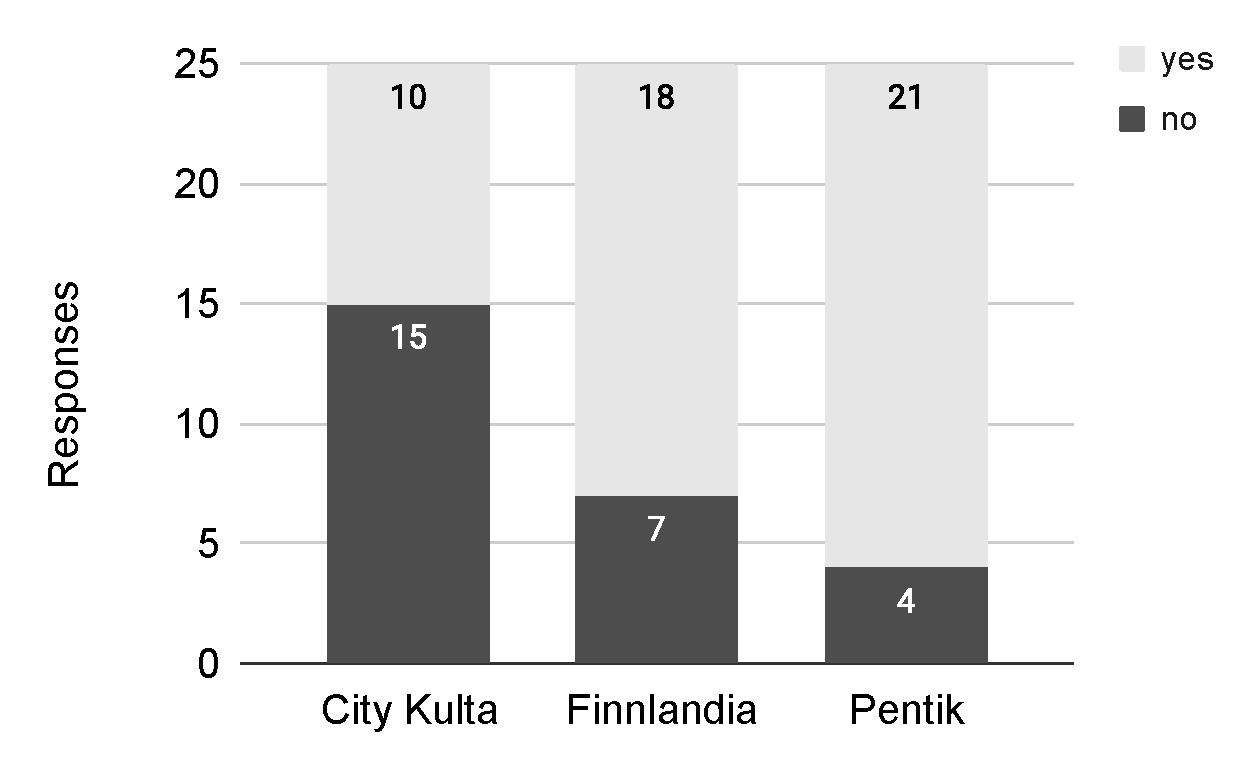
\includegraphics[width=0.49\linewidth]{figures/chapter3/resp_stores_Q2.pdf}}
	\caption{Stack column charts representing the participants answers to the two questions of the additional questionnaire, classified into ``Yes'' and ``No'', according to the store.}
	\label{chap8:fig:stores_comp_QA}
\end{figure} 


\subsubsection{Video Observation}
Similarly to the analysis for the additional questionnaire, the Cochran's Q test was used to compare between the conditions, the answers (``Yes'' or ``No'') given to the robot during the task when it asked them if they had understood (see Figure~\ref{chap8:fig:comp_video}). The analysis rejected the independence between the given answer and the condition ($p<0.01$). According to post-hoc comparisons using the McNemar's test, the difference is significant between condition 1 and 2 ($p<0.05$), but not between condition 1 and 3 and between condition 2 and 3. Thus, participants appear to understand Pepper's directions better in Condition 2 than in Condition 1.

\begin{figure}[!hbt]
	\centering
	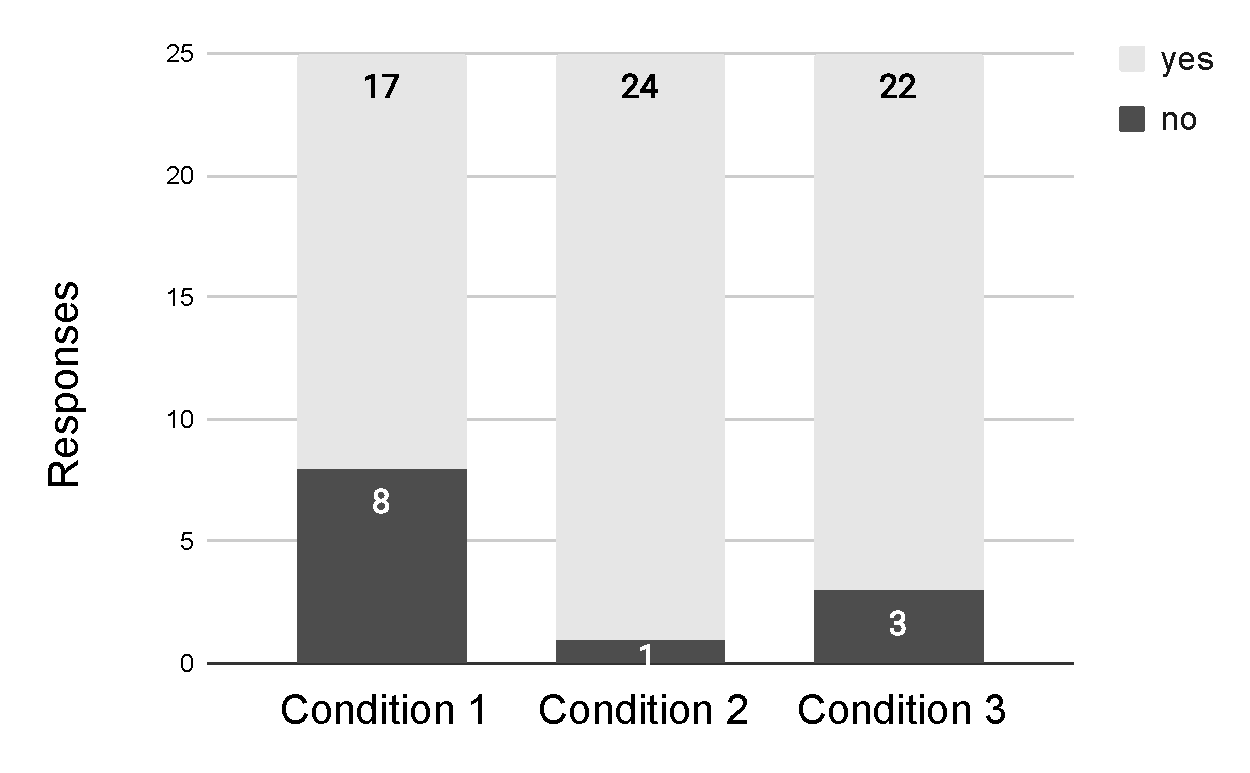
\includegraphics[width=0.49\linewidth]{figures/chapter3/resp_video.pdf}
	\caption{Stack column chart representing the participants answers to the question asked by Pepper after it explained the route, according to the condition.}
	\label{chap8:fig:comp_video}
\end{figure} 

For each condition, we were interested in the percentage of time the participants spent looking in the direction of the path to be taken relative to the total interaction time of the given condition (see Figure~\ref{chap8:fig:look_video}). 

\begin{figure}[!htb]
	\centering
	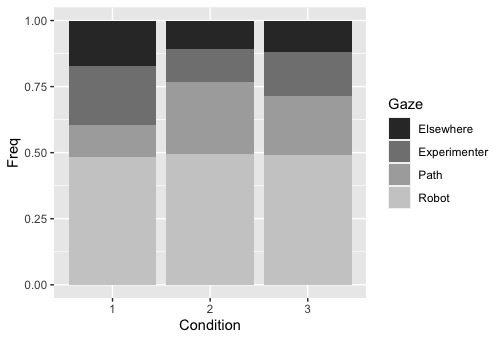
\includegraphics[width=0.8\linewidth]{figures/chapter3/freqRegard.jpeg}
	\caption{Relative frequencies of gaze direction according to the condition.}
	\label{chap8:fig:look_video}
\end{figure} 

The data do not follow a normal distribution, which requires the use of non-parametric tests. Friedman's test reveals an effect of the condition on the percentage of time spent looking in the direction of the path ($F=20.33, p<.01$). Wilcoxon tests show a significant difference between condition 1 and 2 ($p<.01$) and between condition 1 and 3 ($p<.01$). There was no significant difference between condition 2 and 3.

Finally, other analyses are presented in Table~\ref{chap8:tab:proba_video}.

\begin{table}[]
	\centering
	\resizebox{\textwidth}{!}{%
		\begin{tabular}{l||c|c|c}
			
			\multicolumn{1}{c||}{Probabilities to have}                                                                                             & Condition 1 & Condition 2 & Condition 3 \\ \hline\hline
			the sequence ``Robot-Chemin-Robot'' for the gaze                                                                              & 28\%         & 80\%         & 84\%         \\ \hline
			the participants spontaneously moving                                                                                         & 8\%          & 64\%         & 32\%         \\ \hline
			the participants moving on robot request (Cond. 3 only)                                                                       & -           & -           & 24\%         \\ \hline
			\begin{tabular}[c]{@{}l@{}}the participants spontaneously moving and then \\ moving on the robot request (Cond. 3 only)\end{tabular} & -           & -           & 20\%         \\ 
		\end{tabular}%
	}
	\caption{Probabilities that the selected behaviors arise according to the conditions, based on video analysis.}
	\label{chap8:tab:proba_video}
\end{table}

\subsubsection{Interview}

18 participants perceived the difference between all conditions (see Figure~\ref{chap8:fig:interview_diff}), and the other 7 perceived only the difference between condition 1 and the other two conditions. 13 participants preferred Condition 2, 8 participants preferred Condition 3, and 4 preferred Condition 1 (see Figure~\ref{chap8:fig:interview_pref}). Condition 1 seemed to be the least preferred (14 participants, compared to 3 for condition 2 and 4 for condition 3) (see Figure~\ref{chap8:fig:interview_least}).

9 participants indicated that they liked the fact that Pepper was pointing the way. 7 participants mentioned being disturbed by the robot's movement in condition 3 (``confusing'', ``weird'', ``scary'', ``unexpected'', ``unnatural''), but 4 participants said they liked the fact that the robot was moving (``natural'', ``good'', ``appropriate'').

\begin{figure}[!htb]
	\centering
	
	\subfloat[]{\label{chap8:fig:interview_diff}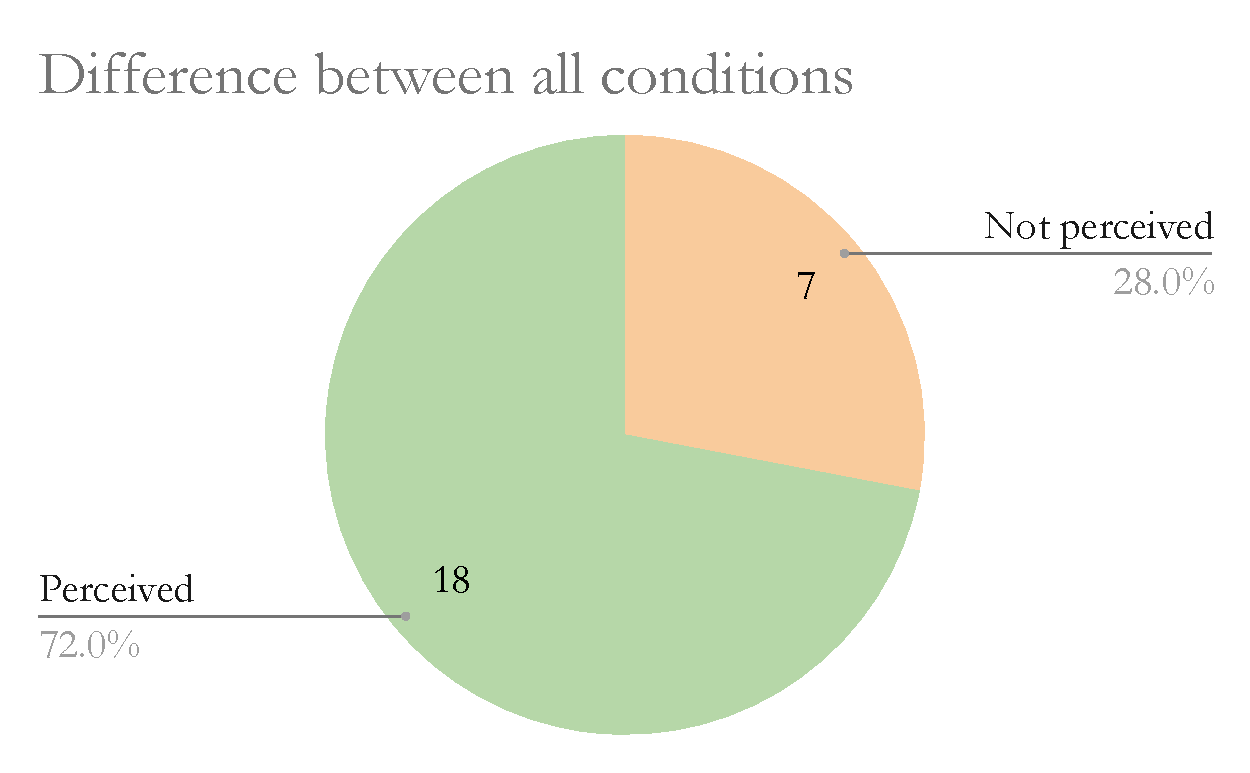
\includegraphics[width=0.49\linewidth]{figures/chapter3/Difference_conditions.pdf}}\hfill
	
	\subfloat[]{\label{chap8:fig:interview_pref}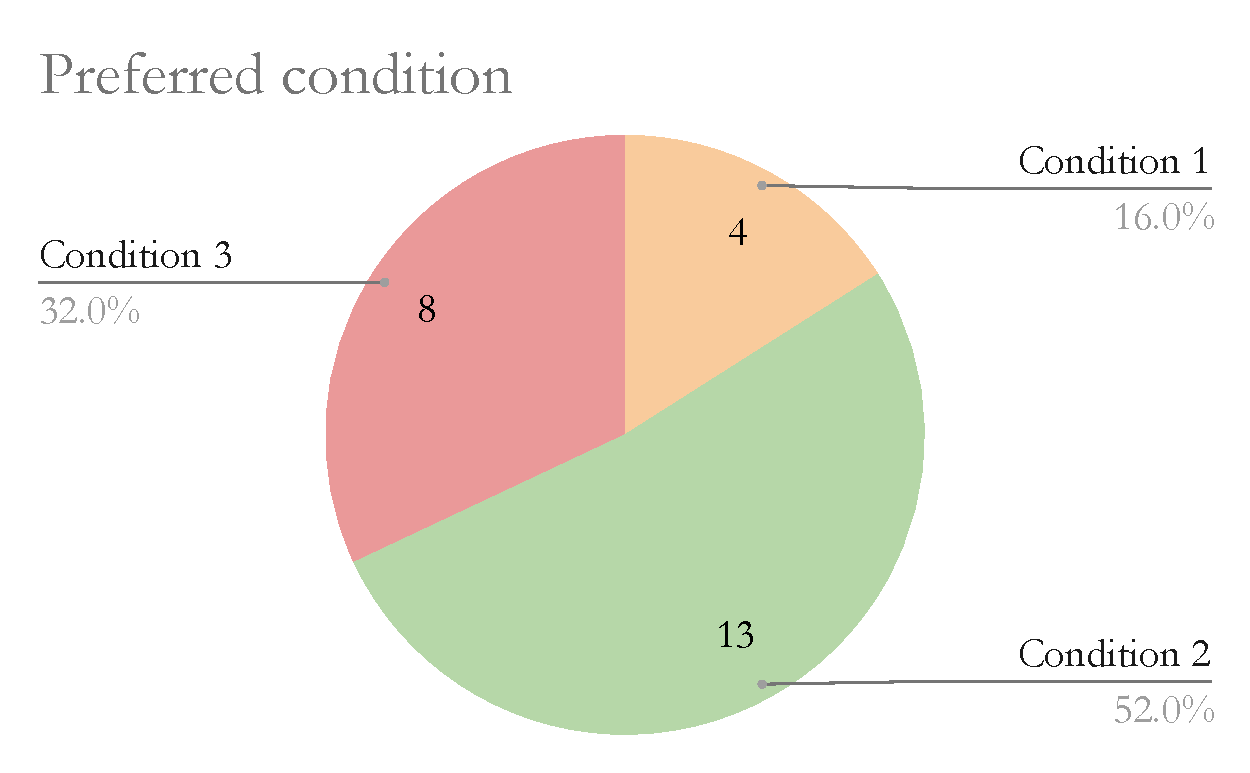
\includegraphics[width=0.49\linewidth]{figures/chapter3/Preferred_condition.pdf}}\hfill
	\subfloat[]{\label{chap8:fig:interview_least}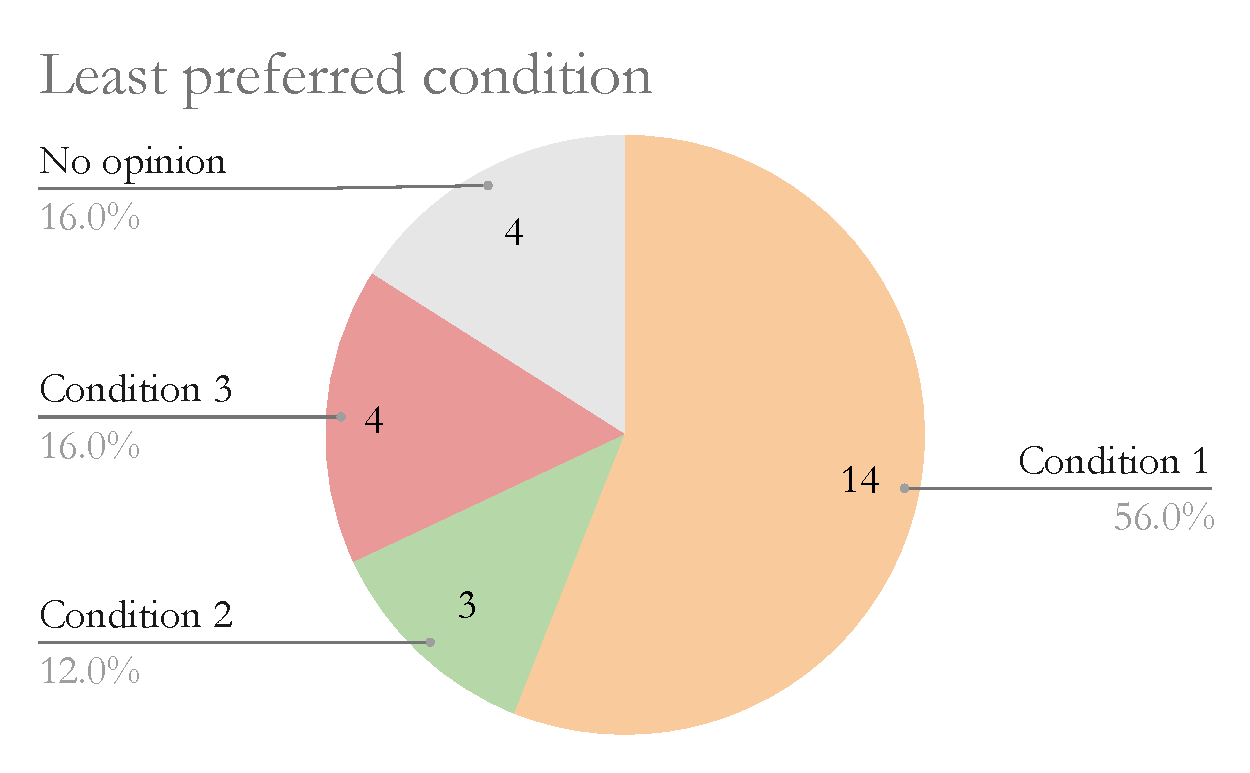
\includegraphics[width=0.49\linewidth]{figures/chapter3/Least_preferred_condition.pdf}}
	\caption{Pie charts representing what said the participants about the conditions.}
	\label{chap8:fig:interview}
\end{figure} 

\subsection{Discussion}

We thought the Condition 3 would be preferred by the participants over the Conditions 1 and 2. However, the results obtained from the 2 questionnaires and the video coding showed that it was not completely the case. But, we can see that Condition 1 was less efficient as a significant number of participants did not understand the directions (15 over 25 participants). Moreover it was poorly evaluated by the participants compared to the Condition 2 and 3 (interaction scores were lower for the Condition 1). Such results highlight the need for the pointing, enabling a shared perspective but they do not indicate that a more refined one as in Condition 3 is necessary.

At first, these results can be seen as a disappointment for our complete system but actually they are a rich source for improvement, starting with the human-aware navigation. Indeed, from the interviews, it stood out that the fact the robot moves, the way the robot moves was something disturbing (7 participants mentioned it). One of the reason was that the robot often span round. We were aware of the issue before the user study, tried to correct it but we realized it was not enough. As the deployed system presented in Section~\ref{subsec:archi-integration} had to leave out navigation for safety reason, it had not been tested as extensively as the other components. It would have been the opportunity to better refine the costs and constraints values of the component.

Thus, it would be interesting to perform a new user study comparing the Conditions 2 and 3 but with an improved navigation or different mode of the navigation. And so, to observe if the Condition 3 has still no significant difference with the Condition 2. It would probably not change in term of comprehension but  it would probably improve the perceived quality of the interaction in the Condition 3. In this case, it would be valuable to keep the task proceeding of Condition 3 as offering a better experience to customers.

Video analyses give some idea to take into account other elements than verbal communication when the robot wants to know if the human understood its explanations or not. Indeed, participants tended to look more frequently elsewhere in Condition 1 than in Condition 2 and 3 (even though not statistically significant). Helped with a software recognizing gaze directions, it would be an interesting information to take into account for the supervision.


\section{Integration and test of the QoI Evaluator}\label{sec:qoi_integration}
As a proof-of-concept for the QoI Evaluator presented in Chapter~\ref{chapter:chap7}, we integrated it in the direction-giving task described in this chapter. It is also an excerpt of the paper accepted in the Journal of Social Robotics~\cite{mayima_2021_towards}.

More specifically, this implementation of the Quality of Interaction Evaluator measured the interaction quality at the direction-giving task level and at the elementary actions level, omitting the interaction session level as this latter was not our focus in the \acrshort{mummer} project. The QoI Evaluator was integrated into the Supervisor presented in this chapter. The QoI Evaluator is implemented as an \acrshort{rja}. After multiple testings, we reached the conclusion that it was pertinent, at least in the context of the direction-giving task, to have the Evaluator computing the QoI every second for both levels. Therefore, every second, the system computes the value of each metric and then outputs a value for $QoI_{task}$ and $QoI_{action}$. 

\begin{figure}[!htp]
	\subfloat[A customer listening to Pepper after re-positioning]{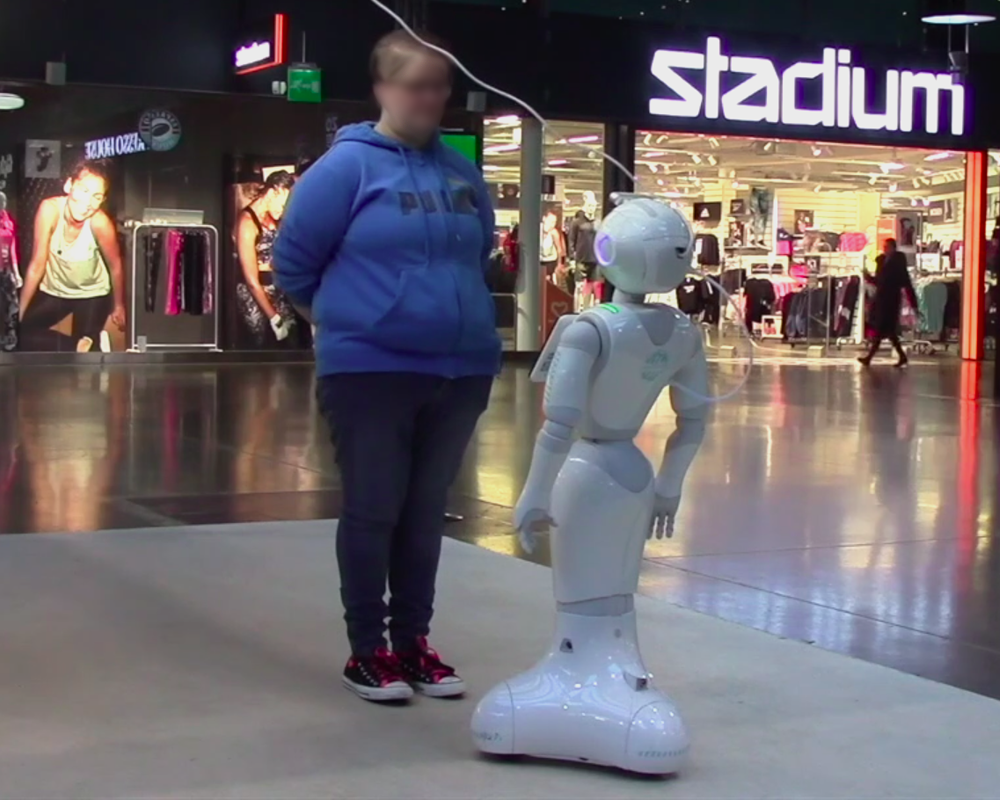
\includegraphics[width=0.49\linewidth]{figures/chapter3/human_1_mall.png}}\hfill
	\subfloat[A customer listening and Pepper pointing to a corridor]{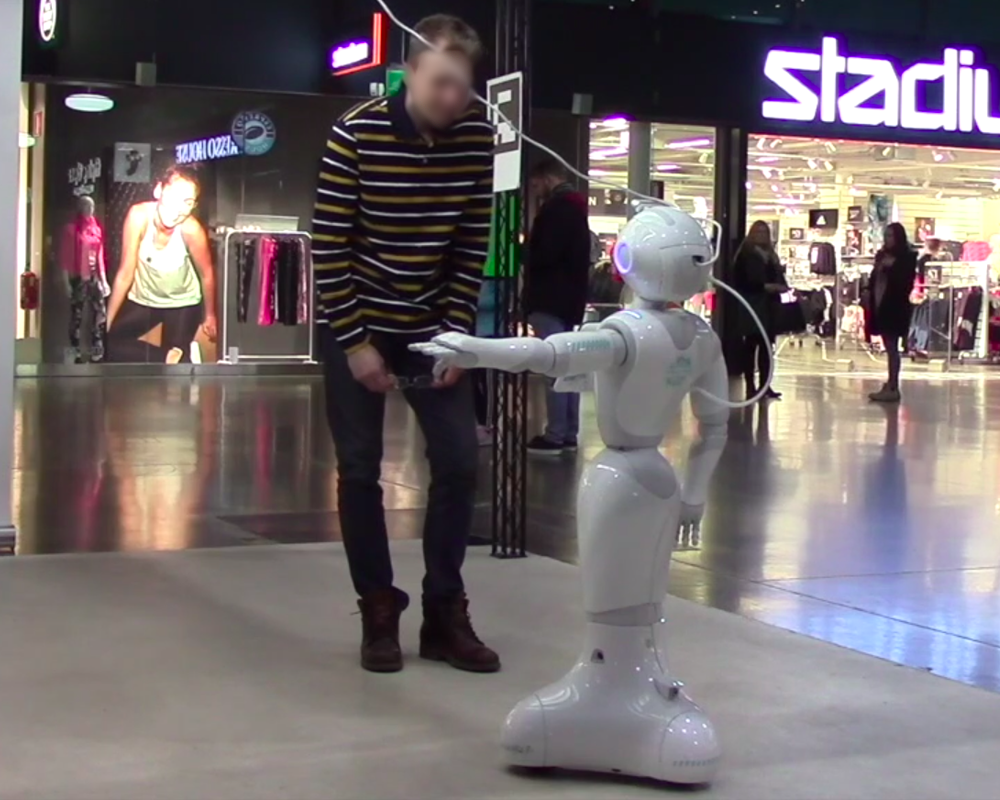
\includegraphics[width=0.49\linewidth]{figures/chapter3/human_2_mall.png}}\hfill
	\subfloat[A customer answering to Pepper]{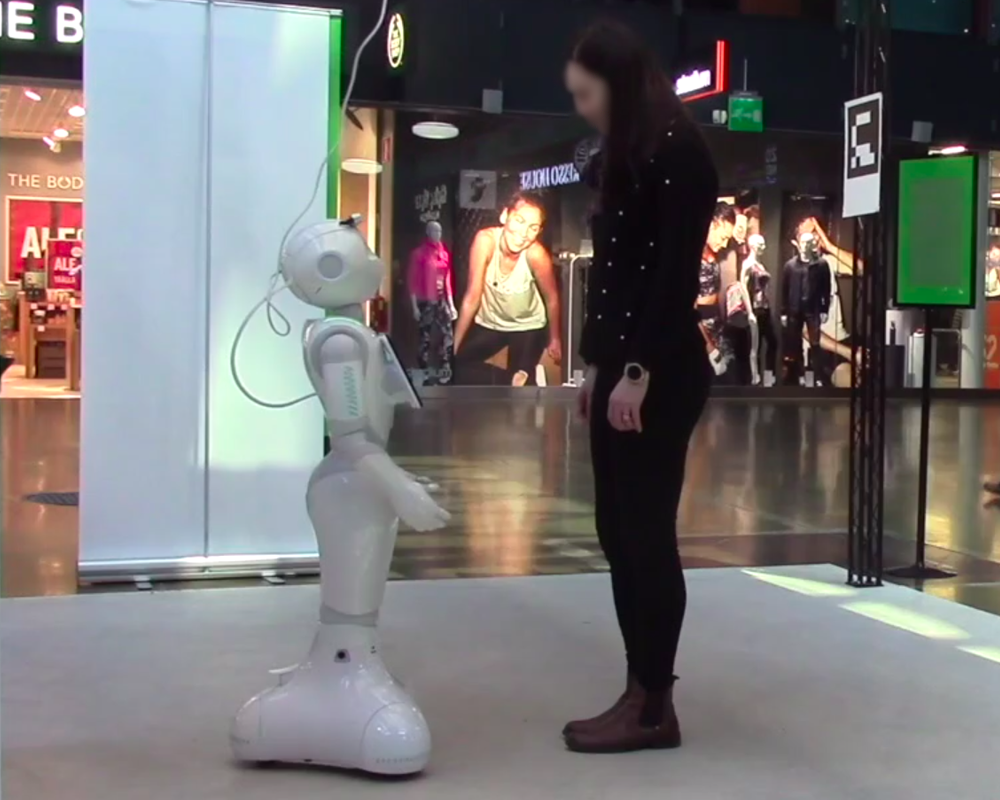
\includegraphics[width=0.49\linewidth]{figures/chapter3/human_3_mall.png}}\hfill
	\subfloat[A customer listening and Pepper pointing to a shop]{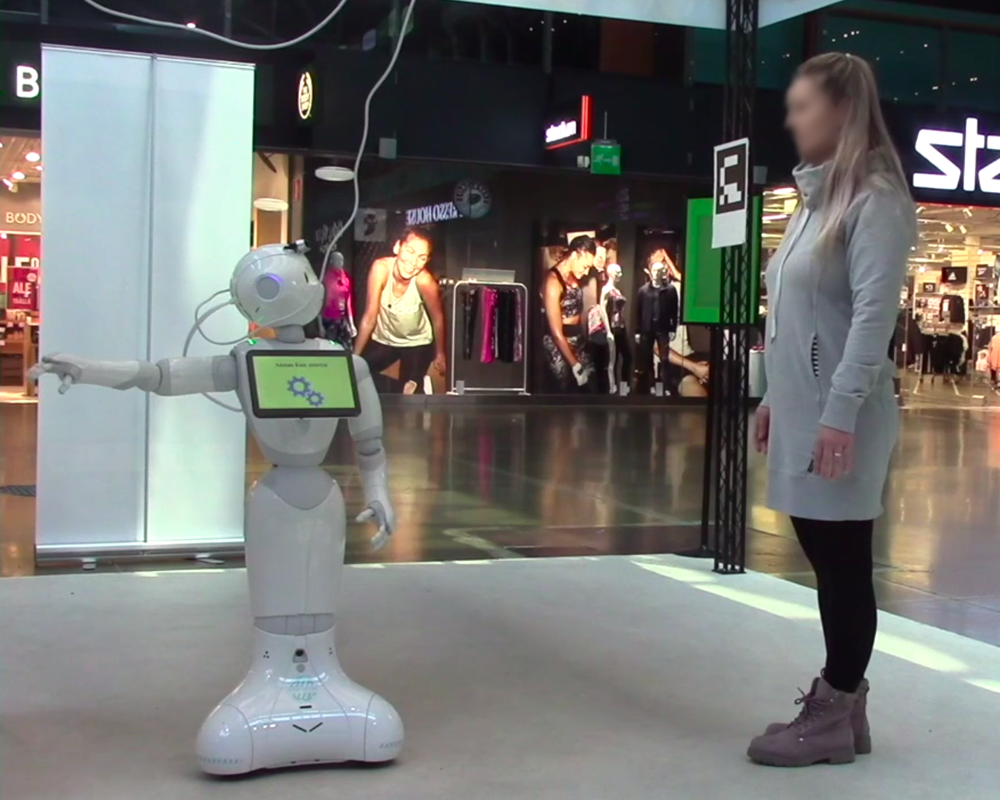
\includegraphics[width=0.49\linewidth]{figures/chapter3/human_4_mall.png}}\hfill
	\caption{MuMMER robot engaged in direction-giving tasks. Around 350 trials with customers in the mall allowed us to gather empirical data to select the metrics and tune the measuring functions parameters.}
	\label{fig:customers}
\end{figure}

As mentioned in the step \ref{list:mall} of the chronicle, the robot interacted in the wild with dozens of usual customers (Fig.~\ref{fig:customers}), executing around 350 direction-giving tasks. This allowed us to improve the performance of the direction-giving task, to gather standard durations of the subtasks executions and to draw lessons about metric definitions and choices (\eg we realized it was not relevant to measure the human visual attention towards the robot when it was giving the route explanation as humans look around at this moment). Unfortunately, the practical conditions of the project deployments did not offer us the possibility to evaluate the QoI Evaluator based on a study in the mall with real customers. So, we demonstrated -- after improvements of the metrics equations such as the Distance-to-Goal one, and manual tuning of their parameters based on the experience in the mall -- our finalized concept through tests in our lab (step~\ref{list:refin}). This is shown in Sect.~\ref{subsec:results} where we present and discuss, a comparison of the QoI computed by the robot when it is dealing with an ``ideal'' human, a ``confused'' human and a ``non-compliant'' human during a direction-giving task, performed in the lab. Before that, we present in Sect.~\ref{subsec:task_qoi} and Sect.~\ref{subsec:action_qoi} how the QoI is evaluated at both task and action levels for the direction-giving task.

\subsection{QoI Evaluation at the task level}\label{subsec:task_qoi}

In the context of the direction-giving task, we have selected two metrics to evaluate the QoI at the task level: a metric defined in the Sect.~\ref{sec:metrics}, the \emph{Deviation from standard duration} and, the aggregation over time of the actions QoIs. Following the process of Fig.~\ref{fig:qoi_schema}, we measure the QoI of the $\text{Task}_i = \text{direction-giving\_task}$, based on the QoI of all task actions and $\text{Task metric}_1$ = Deviation from standard duration.

The \emph{Deviation from standard duration} is used to measure the QoI at the task level as the task is a sequence of subtasks. Indeed, if the subtask lasts longer than expected, the QoI should decrease. Then, as needed for the metric computation we have determined the values of the soft deadlines $SD_i$ for each subtask $a_i, i \in [0,4] $, using the empirical data we gathered as explained in Section~\ref{subsec:deploy}. Specifically, we have computed the average time execution of each subtask, after removing the cases for which the execution of the subtask was annotated as not smooth. These soft deadlines are presented in table~\ref{tab:dl}. Finally, we chose $V_i=0.5$ for all the subtasks.
\begin{table}[ht]
	\centering
	\begin{tabular}{l|c}
		\hline
		Subtasks & soft deadline (s) \\ 
		\hline
		Target refinement process &  30 \\ 
		Ensuring Correct HR Placement   & 30 \\ 
		Ensuring target seen  & 20 \\ 
		Direction explanation and pointing & 30 \\
		Ensuring Direction Seen & 20\\
		\hline
	\end{tabular}
	\caption{Soft deadlines $SD_i$ for each subtask of the direction-giving task}
	\label{tab:dl}
\end{table}

The task QoI is also dependent on the actions QoI values (their computation is described in Sect.~\ref{subsec:action_qoi}). Indeed, the actions QoIs should be reflected on the task QoI as, if a majority of the actions have a low QoI, the task QoI cannot remain high. That is why, besides the\emph{ Deviation from standard duration}, we take into account the average of the action QoIs of the actions already executed or still running.

Then, the task QoI is computed using Equation~\eqref{eq:qoi} presented in Sect.~\ref{sec:eval}. After various trials we have empirically chosen the weights $W_i$ for each metric $M_i, i \in [0,1]$. The final equation to compute the task QoI is:
\[QoI_{dir-giv\_task}(t)=\frac{ \Phi_{dir-giv\_task}(t) + 3 * \overline{QoI}_{actions} }{4}\]

\subsection{QoI Evaluation at the action level}\label{subsec:action_qoi}
As mentioned earlier, each subtask of the direction-giving task can be decomposed into actions. These actions involve several turn-taking steps, the robot asking complementary information, informing the human or expecting an action or reaction from them. We need to measure the QoI during the execution of each action. To do so, we have chosen one or more metrics for each action. 

For each action of the following list, we explain which metrics $M$ of Table~\ref{tab:metrics_impl} we have used and scaling functions of Appendix~\ref{annex:functions} and then, how we compute the action QoI. Finally, the ways metrics are aggregated for each action, outputting QoI values, are summarized in Table~\ref{tab:qoi}.

\begin{table}[!hbt]
	\centering
	\begin{tabular}{|p{3.5cm}|c|}
		Action & QoI formula (metric aggregation) \\ \hline \hline
		Robot-Human information sharing & $ M_{Exp\_SI}(t)$ \\ \hline
		Human-Robot Q/A process & \(\displaystyle\frac{M_{Exp\_SI}(t) + M_{H\_contrib}(t) }{2}\) \\ \hline
		Ensuring  that  Human  moves  aside  & \(\displaystyle\frac{M_{DtG}(t) + M_{H\_contrib}(t) }{2}\) \\ \hline
		Human-aware robot navigation  & $M_{TtG}(t)$ \\ \hline
		Ensuring correct human placement for verbal interaction & $M_{H\_contrib}(t)$ \\ \hline
		Ensuring correct human placement for route explanation & \(\displaystyle\frac{M_{DtG}(t) + M_{H\_contrib}(t) }{2}\) 
	\end{tabular}
	\caption{QoI computation for each action as an aggregation of metrics}
	\label{tab:qoi}
\end{table}

\begin{enumerate}[label=(\alph*)]
	\item \label{list_act:info} \emph{Robot-Human information sharing: }The robot speaks to the human, shares information such as the route direction and announces the next steps of the plan. The robot expects that they are paying attention to it. Therefore, we use the \emph{Fulfilling robot expectations about social interaction} $M_{Exp\_SI}$ based on the attention ratio. Two parameters need to be defined for the scaling function, the bounds $b_1$ and $b_2$. As the minimum value for the metric, a ratio, is 0 and the maximum value is 1, then $b_1=0$ and $b_2=1$. 
	The QoI of the action is computed with this only metric.
	
	\item \label{list_act:qa} \emph{Human-Robot Q/A process: } The robot asks a question to the human. As for the previous action, the robot expects the human to pay attention to it so we compute the QoI with $M_{Exp\_SI}$. It also expects the human to give an appropriate answer. If it does not happen, it will ask the human to repeat, specifying that the answer has not been understood. We have limited the possible number of attempts to 3. After 3 attempts, the robot ends the task, as it cannot carry on with the task without an answer. So, we use \emph{Human contribution to the goal} $M_{H\_contrib}$, the number of times the robot repeats. Because the maximal number of repetitions is 3, we set for the scaling function $b_1=3$ and $b_2=0$.
	
	The QoI is computed with the two metrics: \emph{Fulfilling robot expectations about social interaction} and \emph{Human contribution to the goal}.
	The trials showed that the action QoI results were satisfying with the weights $W_i=1, i \in [0,1]$ as applying the Equation~\eqref{eq:qoi}.
	
	\item \label{list_act:moves_aside} \emph{Ensuring that Human  moves aside: }This action is used if, for pointing, the robot decides to place itself in a position which is very close to where the human is currently standing. In this case, the robot asks the human to step aside to the right or left, depending on the human's future position. Then, we want to measure the progress of the human going further from the planned robot position. In order to do this, we use the \emph{Distance-to-Goal} $M_{DtG}$ but with the condition of the $\Delta DtG$ equation adapted, being $\text{if } path\_length(t) >  path\_length(t-1)$ instead of $\text{if } path\_length(t) <  path\_length(t-1)$. We scale the metric with  $-s_1$, the additive inverse of the scaling function and not directly $s_1$ as the closer to 0 $\Delta DtG$ is, the better it is in terms of goal completion. From trials, we set $-s_1$ parameters values with $th=5$ and $k=1.5$.
	
	If the human does not move or does not go far enough from the robot position, the robot will ask again with a limit of 3 trials (if the robot cannot move, it will carry on the task from their current positions). So, we use $M_{H\_contrib}$ as for the previous action. 
	
	\item \label{list_act:nav} \emph{Human-aware robot navigation: }The robot has to move from its initial position to its computed one. It navigates while respecting social constraints and its path may change as it adapts according to what the human is doing. At execution time, to measure the robot progress towards its goal, we use the \emph{Time-to-goal} $M_{TtG}$, with the same scaling function than $M_{DtG}$. The QoI of the action is computed with this only metric. 
	
	\item \label{list_act:correct_place1} \emph{Ensuring correct human placement for verbal interaction: }After it has moved, the robot asks the human to come in front of it. If the human is not perceived after a few seconds, the robot will ask again and so on in a maximum of 3 trials. If after these 3 times the human is still not perceived, the robot ends the task. 
	
	The QoI of this action is computed with $M_{H\_contrib}$ -- we do not use $M_{Exp\_SI}$ as the human is not in the field of view when the robot is calling them.
	
	\item \label{list_act:correct_place2} \emph{Ensuring correct human placement for route explanation: }Once the human is in the robot field of view after the HR motion, they may not be at the right place to properly see what the robot has to point at. In this case, the robot will ask the human to move forward or backward according to what it has computed about the human perspective (\eg this is to avoid that an object occludes the view for the human). Then, we want to measure the human progress towards the position the robot has computed for them. In order to do this, we use the \emph{Distance-to-Goal} $M_{DtG}$.
	
	The robot stops giving instructions if it computes that the position of the human allows them to see the target, or after 3 trials, so we use $M_{H\_contrib}$. After 3 trials, if the human cannot see the target, still, the robot will carry on the task taking this into account.
	
	
\end{enumerate}


\begin{landscape}
	\setlength\tabcolsep{1.5pt}
	\begin{table*}[ht]
		\centering
		\begin{tabular}{|c|p{1.5cm}|c|c|}
			Metric id & Metric name & Metric equation -- with Equations of Section~\ref{sec:metrics} & Scaled metric -- with functions of Appendix~\ref{annex:functions} \\\hline\hline
			
			\(\displaystyle M_{H\_contrib}\)
			& Human contribution to the goal 
			& \raisebox{-0.5cm}{ \(\displaystyle nb\_R\_repet \)} &  \raisebox{-0.5cm}{ \(\displaystyle n_1(nb\_R\_repet) = 2 * \dfrac{nb\_R\_repet-3}{-3} -1 \)} \\\hline
			
			\(\displaystyle M_{Exp\_SI}\)
			& Fulfilling robot expectations about social interaction 
			&    \raisebox{-0.5cm}{ \(\displaystyle Ar = \frac{duration_{isAttentiveTo(robot)=true}}{duration_{robot\_speaks}} \) }
			&  \raisebox{-0.5cm}{\(\displaystyle n_1(Ar) = 2 * Ar -1 \)} \\\hline
			
			\(\displaystyle M_{DtG}\)
			& Distance-to-Goal & 
			\(\displaystyle \left\{
			\begin{array}{ll}
			\Delta DtG(t=0) = 0\\
			\begin{aligned}
			\Delta& DtG(t) = \max(0,\Delta DtG(t-1) - 1)  \\&\text{if } path\_length(t) <  path\_length(t-1) \\
			
			\end{aligned}\\
			\Delta DtG(t)= \Delta DtG(t-1) + 1, \text{otherwise.}
			
			\end{array}
			\right.
			\)
			&   \(\displaystyle -s_1(DtG(t)) = -1 + 2 \exp{\left(-\ln{(2)}\left(\dfrac{DtG(t)}{5}\right)^{1.5}\right)} \) \\\hline
			
			\(\displaystyle M_{TtG}\)
			& Time-To-Goal & 
			\(\displaystyle \Delta TtG(t) = \max(0, e(t)  + TtG(t) - TtG(T_0)) 
			\)
			&  \(\displaystyle -s_1(TtG(t)) = -1 + 2 \exp{\left(-\ln{(2)}\left(\dfrac{TtG(t)}{5}\right)^{1.5}\right)} \) \\
			
			
		\end{tabular}
		\caption{Metrics used in the implementation presented in Section~\ref{sec:qoi_integration}.}
		\label{tab:metrics_impl}
	\end{table*}  
\end{landscape}

\begin{figure*}[!ht]
	\centering
	\subfloat[Evolution over time of the measured QoI for the 'ideal' human. Both action and task QoIs remain at 1 as the task is proceeding smoothly. ]{\label{fig:human_ideal}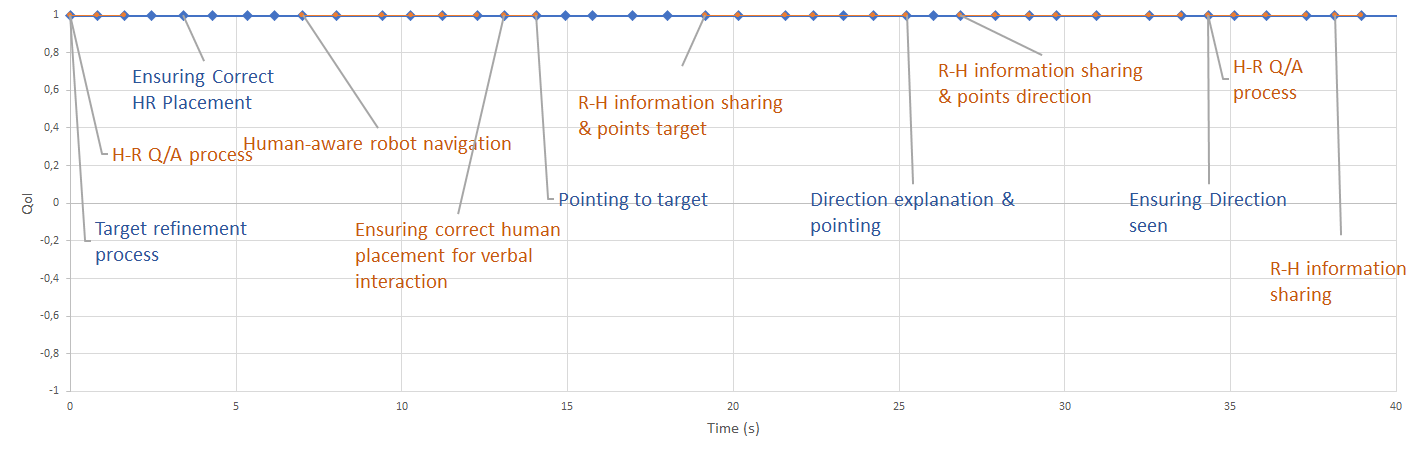
\includegraphics [width=\linewidth]{figures/chapter3/human_ideal.png}}\hfill
	\subfloat[Evolution over time of the measured QoI for the ``confused'' human. They took time to answer the first robot question and to move forward but the task QoI does not drop too much because the robot was able to give the route explanation without any issue even though the human was not very attentive. ]{\label{fig:human_confused}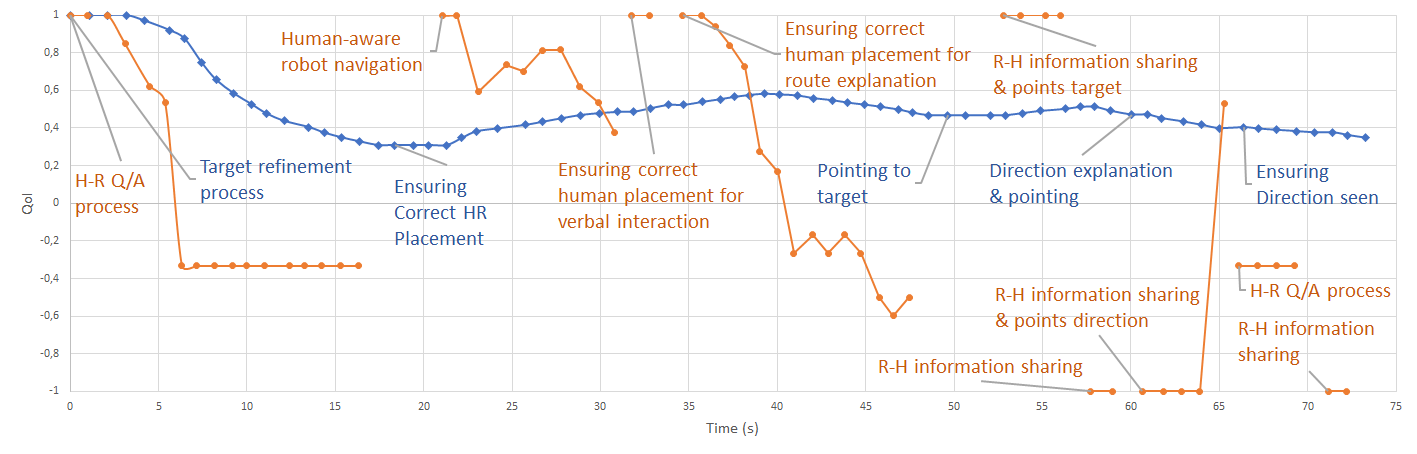
\includegraphics[width=\linewidth]{figures/chapter3/human_confused.png}}\hfill 
	\subfloat[Evolution over time of the measured QoI for the non-compliant human. Several times the human did not give the expected answer to the robot during the target refinement process. Then, they blocked the robot path. After that, the robot had to ask twice the human to come in front of it. Finally, the robot repeated the route direction three times but still the human kept saying that they did not understand. Therefore, the task QoI decreases all along the task.] 
	{\label{fig:human_not_comp}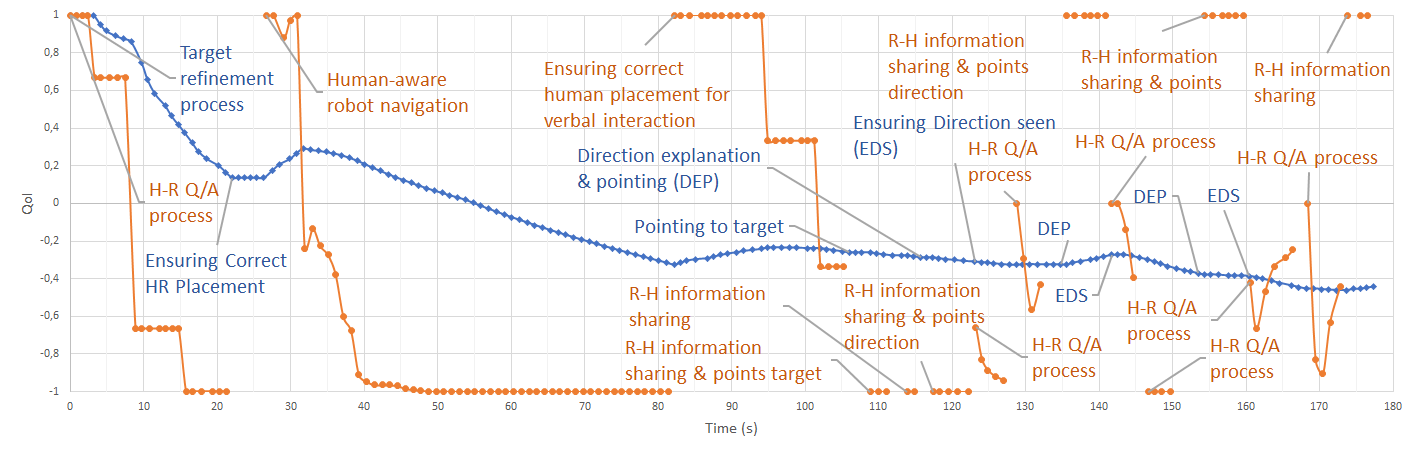
\includegraphics[width=\linewidth]{figures/chapter3/human_not_comp.png}}\hfill
	\caption{Evolution over time of the measured QoI for the route guidance task with three different human behaviors. The QoI for the task is drawn in blue, and the QoI for the actions is drawn in orange.}
	\label{fig:impl_qoi}
\end{figure*}

\subsection{Proof-of-Concept}\label{subsec:results}
This section reports on an effective implementation of the approach as an illustrative proof of concept. We show the ability of the robot to conduct an interactive task, to assess in real-time the QoI and to track its evolution during three direction-giving task executions where the same human displayed a different way of behaving. In the three cases, the task was conducted until its end, in our lab where we reproduces the mall environment (Fig.~\ref{fig:chap3_lab}, Table~\ref{tab:malls}). The computed QoI for each way is presented in Fig.~\ref{fig:impl_qoi}. The three different ways of behaving are described in the following list:
\begin{bulletList}
	\item A human executed perfectly the expected actions and was not disturbing the robot when it navigated (\ie the ``ideal'' human from the robot point of view). 
	\item A bit ``confused'' human tried to contribute to the task success but did not execute everything well. The human was, from time to time, not very attentive, as looking around. Also, they gave an answer to the first question that the robot did not understand, and then they took their time before answering again. Then, they prevented a bit the robot to move as it had planned and once the robot reached its position, they took time to come as close as the robot wanted. 
	\item A human wanted to disturb the robot during the task. They gave three incomprehensible answers to the first question, blocked multiple times the robot in its move, waited for the robot to ask twice to come in front of it and finally asked the robot to point and explain the route three times. 
\end{bulletList}

\begin{table}[!h]
	\begin{center}
		\begin{tabular}{ | c || c | c | }
			\hline
			Mall elements                   & Mockup mall & Real mall \\ \hline \hline
			Shops              & 19            & 140   \\ \hline
			Doors, stairs, elevators & 10            & 50    \\ \hline
			Corridors              & 11            & 41    \\ \hline
			Levels   & 2            & 2   \\ 
			\hline
		\end{tabular}
	\end{center}
	\caption{\label{tab:malls} Number of elements described in the mockup and real malls (geometric, topologic and semantic models in Fig.~\ref{fig:chap3_3Dmodels}).}
\end{table}

Now, if we take a look at the QoI outputs of Fig.~\ref{fig:impl_qoi}, we can see that their three shapes are very different. In Fig.~\ref{fig:human_ideal}, we can observe that the task and actions QoIs remain with the highest value 1 all along. A graph as this one allows us to infer that everything went very smoothly during this direction-giving task. Then, we can guess that it corresponds to the execution performed with the 'ideal' human. 

In Fig.~\ref{fig:human_confused}, we note that each subtask was executed in respect of the standard duration. If the QoI of \emph{Target refinement process} drops it is because of the action QoI as the QoI of the \emph{H-R Q/A process} drops because the robot had to repeat the question and the human was not looking at it. From 21 seconds to 40 seconds, we can see the task QoI getting higher as the QoIs of \emph{Human-aware robot navigation}, \emph{Ensuring correct human placement for verbal interaction} and the beginning of \emph{Ensuring correct human placement for route explanation} are quite high. Next, seeing the shape of the computed QoI of the action \emph{Ensuring human placement for route explanation}, we can infer that the human was not moving as the robot wanted. Indeed, they took 10 seconds to make one step forward (they had 1 meter to cross). Because of that, the task QoI started to decrease again. In the final part of the task, the human was time to time attentive to the robot and answered quickly to the last question, so the task QoI remained rather equal with its final value being $0.34$ which is above 0 so meaning a correct interaction.

\begin{figure}[!t]
	\centering
	\begin{subfloat}[Human who put themselves on the robot path, preventing the robot to navigate towards its goal position]{
			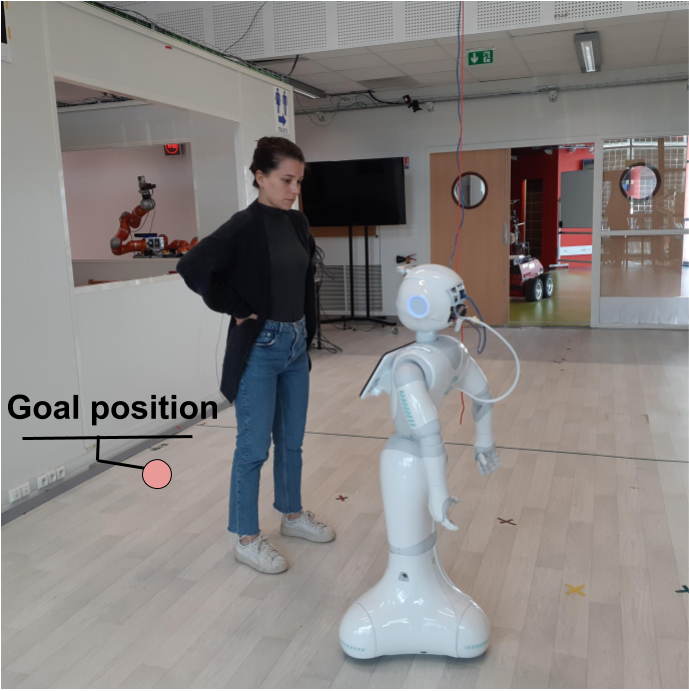
\includegraphics[width=0.29\linewidth]{figures/chapter3/blocking1.png}}\hfill
	\end{subfloat}
	\begin{subfloat}[Human who put themselves on the robot path after it computed a new path to reach its goal position]{
			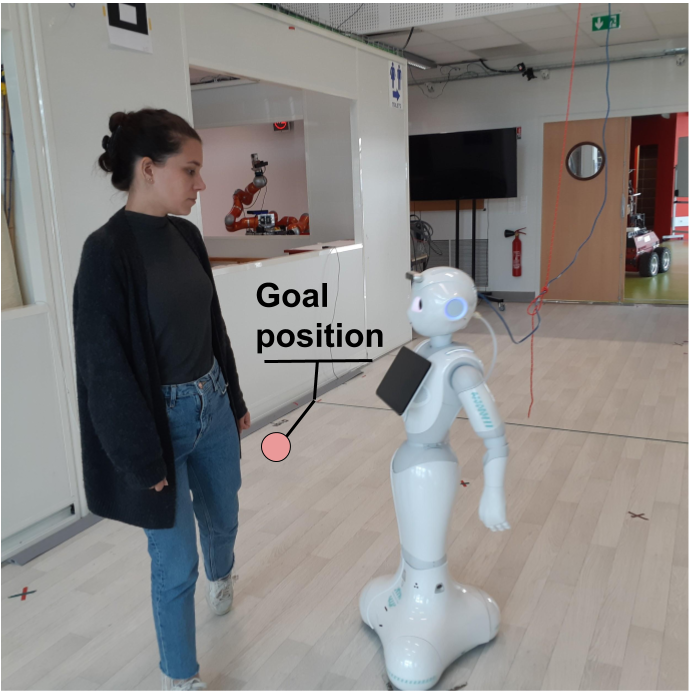
\includegraphics[width=0.29\linewidth]{figures/chapter3/blocking2.png}}\hfill
	\end{subfloat}
	\begin{subfloat}[Human finally getting outside of the robot path, allowing it to reach its goal position]{
			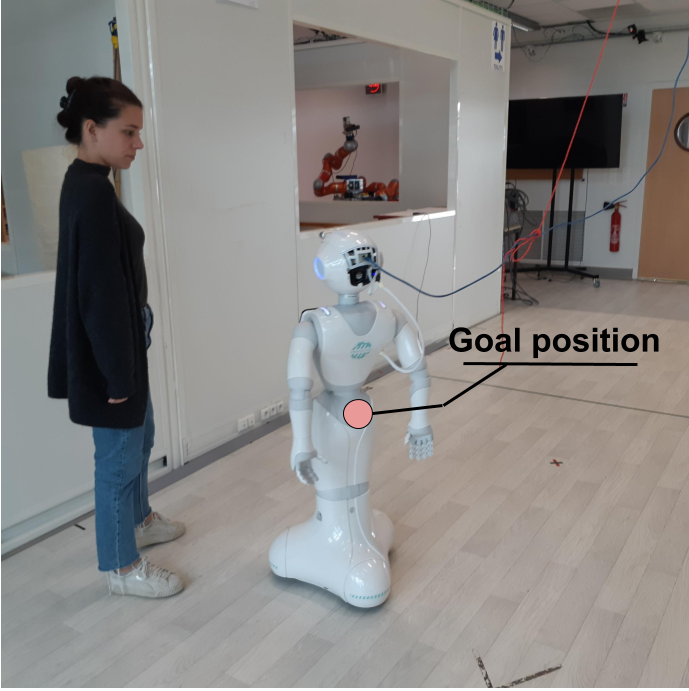
\includegraphics[width=0.29\linewidth]{figures/chapter3/not_blocking.png}}\hfill
	\end{subfloat}
	\caption{A human disturbing the robot during \emph{Human-aware navigation}, preventing it to reach its goal position as planned.}
	\label{fig:blockig_nav}
\end{figure}

Finally, we can see in Fig.~\ref{fig:human_not_comp} that the final QoI of the task is $-0.44$ which allows us to infer that the task was not executed smoothly. And indeed, when we look at the shape of the task QoI, it only went down (or almost) all along the task. It is explained by some subtasks that took more time than they should have and also by some actions QoIs that are very low, especially the one of \emph{Human-aware robot navigation}. At the beginning of the robot navigation, the estimated time to goal returned by the planner was 6 seconds but the robot actually took 50 seconds to reach its goal then the action QoI computed with $=M_{TtG}(t)$ was $-1$ for $40$ seconds. And indeed, all along its navigation, the human was blocking the robot until they got tired of this game, as visible on Fig.~\ref{fig:blockig_nav}.

In this example, we showed the QoI evaluation process integrated to a complete robotic architecture. The robot was able to assess the QoI in real-time while interacting with a human.

\subsection{Discussion on the results of the QoI Evaluator}
While a number of evaluation methods has been proposed to evaluate a human-robot interaction from the human perspective and often for analysis after performance, our choice to let the robot evaluate, on its own and in real-time the quality of its interaction with a human is quite new and original. To endow the robot with such an ability, we designed, implemented and tested a number of metrics and a method to aggregate them.

The work of Steinfeld \etal{}~\cite{steinfeld_2006_common} was very helpful to design a first set of metrics and as an inspiration about what could be used. From there, we have elaborated and proposed a set of metrics which are meant to estimate of the quality of an ongoing interaction and not once it is over. 
The work of Hoffman regarding the \emph{fluency} definition and how to measure it was also inspiring~\cite{hoffman2019}. In a way, we extended his work by giving a meaning to the fluency measurement on the robot side, and in real-time -- while their work applies to offline evaluation of shared workpace tasks. 
In Sect.~\ref{sec:rel}, we mentioned systems measuring human affective states in real-time such as the framework developed by Tanevaska \etal{}~\cite{tanevska:hal-01615491}. Although we think such metric could be an interesting additional information to assess if an interaction is going well, we believe that these measurements do not offer an accuracy that would lead to objective measurement of the quality of interaction, thus, we did not introduce them in our set for now. However, this could be done since our framework is designed to be open to new metrics. 
As for contributions, like the one proposed by Anzalone \etal{}~\cite{anzalone_2015_evaluating}, based on metrics such as gaze, head pose, body pose and response times to measure real-time engagement, we took them into account to some extent. However, the measure of the engagement that we propose should be refined depending on the inputs available on-line to the robot. Moreover, we will investigate how their work could be used in a more general way (\eg depending on the action that should be done and its context, human head pose and body posture could be a good indicator of effectiveness and not only engagement). 

Our intention, when we developed the idea of the Quality of Interaction Evaluation, was to use such computation to feed the decision-making process of the robot and this is what we intend to do in the future. However, such framework can also be used to compare interactions between different humans and/or robots, eventually as a benchmark similarly to the work of Sanchez-Matilla~\cite{sanchez} or as a way for developers to detect repetitive interaction issues with an unsupervised robot in a real-world environment.

As a proof-of-concept, we implemented and deployed a first version of a QoI Evaluator assessing task and actions QoIs. We tested it on an interactive robot dedicated to provide route guidance to customers in a large mall. The approach gave satisfactory results. It showed the potential ability of a robot to detect momentary decreases of the Quality of Interaction and also more serious degradation of it which may need drastic change of behavior for the robot. This is only a first step and it should be validated with a study where we will ask humans to evaluate the quality of their interaction with the robot in a similar manner. The goal will be to analyse and compare this to the evaluation of the interaction quality estimated by our robot and, based on that, investigate potential improvements. 

Finally, we do not claim to have a perfect measure of the Quality of Interaction. However, although the concept of Quality of Interaction is quite abstract, Movellan \etal{} showed that when it is measured by human observers, the inter-observer reliability of the concept is quite high~\cite{movellan2007rubi}. Therefore, we believe we can endow the robot with an effective and pertinent ability aiming at measuring the quality of an interaction. We are aware that the set of metrics we proposed to do so is not exhaustive but the framework is designed to be easily extended with new metrics.

\section{Conclusion}

In this chapter, we presented a direction-giving task performed by the Pepper robot. It is not often that an autonomous robot is deployed in a mall for three months. it was a very enriching experience with three contributions: a robotic architecture dedicated to direction giving, a user study and a proof-of-concept for the \acrshort{qoi} Evaluator.

We elaborated a software architecture embedded in a Pepper robot to provide directions to customers in a mall. It is a form of guiding where the robot does not accompany the persons to their final destination but describes and indicates the route to take while pointing. The robot is able to take into account the perspective of the person it interacts with, leading her, if necessary, to a re-positioning of both agents so that the human can see, or see better, the passage. Thus, they can have a concrete idea about the route they are supposed to follow to reach their destination.

To do so, our approach was largely inspired by joint action concepts and guidelines. We performed a human-human study where a human guide gave directions to a customer and analyzed it, through the filter of joint action theory, to draw concepts and ideas directing the design of our robotic system.

This approach allowed us to create a robotic architecture and to develop and integrate a set of components, each of them having a specific role to play in the direction-giving task. They rely upon two representations of the mall. The Semantic Representation is an ontology representing which merchandises are sold in which shop along with the topology of the whole mall. It allows the system to compute the route by taking into account the interacting human's perspective during their future displacement. Then, the Geometric representation is a 3D model of the surrounding areas of the robot. It is used to find places where the robot can point at the first element of the route while ensuring that the human can see the object of the pointing. All of the components are orchestrated through the Supervisor integrating joint action by taking into account human perspectives in different ways (\ie the human orientation along the route (what is on is left/right) and the landmark visibilities) and managing the collaborative execution of shared goals and their associated shared plan, based on an estimation of the human knowledge, and verbal and non-verbal communication.

The robot could perform efficiently the guiding task repeatedly and in autonomy as it has been deployed in a real-world environment for three months. This valuable experience also allowed us to detect and fix bugs we would not have detected and to adjust the guiding task algorithm according to the users' oral feedbacks during deployments. 

Even though we had carefully designed the task with the help of psychologists, it was not enough as the user study showed that the robot moving to improve the shared perspective was not preferred to the robot only pointing. It is a good lesson showing that iterative design is important. However, it is not always easy to be in the conditions to extensively test the system in a real-world environment. Indeed, the robot version used during the three-months deployment was without the navigation. Though, we probably missed some debugging opportunities such as realizing that the robot was spinning so much.






\ifdefined\included
\else
\bibliographystyle{acm}
\bibliography{These}
\end{document}
\fi